\documentclass[12pt]{report}
\usepackage[utf8]{inputenc}
\usepackage[vietnamese]{babel}
\usepackage{amsmath, amssymb}
\usepackage{graphicx}
\usepackage[hidelinks]{hyperref}
\usepackage{caption}
\usepackage{float}
\usepackage{geometry}
\usepackage{tikz}
\usepackage{xcolor}
\usepackage{array}
\usepackage{longtable}
\usepackage{multirow}
\usepackage{fancyhdr}
\usepackage{setspace}
\usepackage{times}
\usepackage{ragged2e}
\geometry{a4paper, margin=2.5cm}
\definecolor{darkblue}{RGB}{0, 0, 139}

% Định dạng tiêu đề section
\usepackage{titlesec}
\renewcommand{\thesection}{\arabic{section}.}
\renewcommand{\thesubsection}{\thesection\arabic{subsection}.}
\renewcommand{\thesubsubsection}{\thesubsection\arabic{subsubsection}.}
\titleformat{\section}{\normalfont\Large\bfseries}{\thesection}{1em}{}
\titleformat{\chapter}[hang]{\bfseries\LARGE}{Chương \thechapter:}{1em}{}
\setcounter{secnumdepth}{22}

\begin{document}

% ======== TRANG BÌA =========
\newgeometry{top=2.5cm,bottom=2.5cm,left=3.5cm,right=2.5cm}
\thispagestyle{empty}

% Vẽ khung viền
\begin{tikzpicture}[remember picture, overlay]
  \draw[line width=1pt, darkblue!50!black]
    ([xshift=2.5cm,yshift=-2cm]current page.north west) rectangle
    ([xshift=-1.5cm,yshift=2cm]current page.south east);

  \draw[line width=3pt, darkblue!80!black]
    ([xshift=2.3cm,yshift=-1.8cm]current page.north west) rectangle
    ([xshift=-1.3cm,yshift=1.8cm]current page.south east);
\end{tikzpicture}

\begin{center}
    \vspace{-0.8cm}
    ĐẠI HỌC BÁCH KHOA HÀ NỘI\\
    TRƯỜNG CÔNG NGHỆ THÔNG TIN VÀ TRUYỀN THÔNG\\
    \rule{0.6\textwidth}{0.4pt} \\[0.9cm]
    
\includegraphics[width=2.5cm]{images/logo.png} \\[1.4cm]
    {\LARGE \textbf{BÀI TẬP LỚN}}\\[0.3cm]
    {\normalsize MÔN: PHÁT TRIỂN ỨNG DỤNG ĐA NỀN TẢNG}\\
    \textit{(Mã học phần: IT4788)}\\[1.6cm]
    \raggedright \textit{\Large Chương 2:}\\
    \begin{center}
        \textbf{\Large TỔNG QUAN VỀ KIẾN TRÚC CỦA DI ĐỘNG}
    \end{center}
\end{center}

\vspace{2.6cm}

\hspace*{0.6cm}
\begin{tabular}{ll}
  \textbf{Nhóm} & \hspace{0.99cm}\textbf{:} 2 \\
  \textbf{Mã lớp học} & \hspace{0.99cm}\textbf{:} 159462 \\
  \textbf{Giảng viên hướng dẫn} & \hspace{0.99cm}\textbf{:} Nguyễn Tiến Thành \\
  \multicolumn{2}{l}{\textbf{Danh sách sinh viên thực hiện:}} \\
\end{tabular}

\vspace{0.3cm}
\renewcommand{\arraystretch}{1.5}

\begin{center}
\hspace*{-0.7cm}
\begin{tabular}{|c|>{\centering\arraybackslash}m{4cm}|c|>{\centering\arraybackslash}m{6.5cm}|c|}
\hline
\textbf{STT} & \textbf{Họ và tên sinh viên} & \textbf{Mã SV} & \textbf{Email} & \textbf{Lớp} \\
\hline
1 & Nguyễn Việt Hoàng & 20215384 & HoangNV215384@sis.hust.edu.vn & IT1-02 \\
\hline
2 & Hoàng Nguyễn Huy & 20215393 & HuyHN215393@sis.hust.edu.vn & IT1-02 \\
\hline
3 & Đỗ Văn An & 20215294 & An.DV215294@sis.hust.edu.vn & IT1-01 \\
\hline
4 & Nguyễn Thị Ngân & 20215436 & Ngan.NT215436@sis.hust.edu.vn & IT1-01 \\
\hline
\end{tabular}
\end{center}

\vspace{1.2cm}
\begin{center}
    \textit{\textbf{Hà Nội, Tháng 4 năm 2025}}
\end{center}

\newgeometry{top=2.5cm, bottom=2.5cm, left=3.5cm, right=2.5cm}

% ========== NỘI DUNG CHÍNH ==========
\tableofcontents
\listoffigures
\listoftables
\justifying

\chapter{Chap1}
\label{chap:Chap1}


\section{Tổng quan về kiến trúc hệ thống}

    Kiến trúc hệ thống là nền tảng quan trọng trong phát triển ứng dụng di động, nơi các thành phần như thiết bị, ứng dụng và server phối hợp hoạt động. Trong phần này, người đọc sẽ tìm hiểu về vai trò của kiến trúc trong việc đảm bảo hiệu suất, khả năng mở rộng và tính ổn định của ứng dụng. Các yếu tố như tính đồng nhất, tính trong suốt và tính khả chuyển sẽ được trình bày như những tiêu chí thiết kế quan trọng. Bên cạnh đó, những mô hình kiến trúc phổ biến và công nghệ hỗ trợ như microservices, containerization, cùng các công cụ DevOps sẽ giúp hình dung rõ hơn về cách xây dựng một hệ thống di động hiện đại và hiệu quả.

    % 1.1.
    \subsection{Tổng quan về kiến trúc hệ thống trong ứng dụng di động}
    \renewcommand{\labelitemi}{--}    
    
    Kiến trúc hệ thống trong phát triển ứng dụng di động là nền tảng kỹ thuật bao gồm ba thành phần chính: phần cứng thiết bị, ứng dụng di động và hệ thống server hỗ trợ phía sau. Mục tiêu chính của kiến trúc này là thiết lập một hệ thống có khả năng vận hành đồng nhất, đảm bảo tính trong suốt giữa các thành phần và đạt được mức độ khả chuyển cao.
    
    \vspace{0.5em}
  
    Việc xây dựng kiến trúc hệ thống hợp lý đóng vai trò quan trọng đối với sự thành công của một ứng dụng. Trước hết, kiến trúc hệ thống ảnh hưởng trực tiếp đến hiệu suất hoạt động cũng như khả năng mở rộng trong tương lai. Bên cạnh đó, một kiến trúc ổn định sẽ giúp ứng dụng hoạt động mượt mà và hạn chế lỗi phát sinh trong quá trình sử dụng. Quan trọng hơn, khi các thành phần trong hệ thống được tổ chức rõ ràng, việc phát hiện và xử lý lỗi sẽ trở nên nhanh chóng và chính xác hơn.
    

    % 1.2.
    \subsection{Các yếu tố quan trọng trong kiến trúc hệ thống}
    \renewcommand{\labelitemi}{--}
    
        Một kiến trúc hệ thống hiệu quả cần đảm bảo ba yếu tố cốt lõi: tính đồng nhất, tính trong suốt và tính khả chuyển.
    
        \vspace{0.5em}
    
        Tính đồng nhất là yêu cầu đầu tiên đối với một hệ thống hiện đại. Để đảm bảo sự nhất quán về dữ liệu giữa client và server, các kiến trúc sư phần mềm thường sử dụng các giao thức và tiêu chuẩn truyền thông như RESTful API hoặc GraphQL \cite{restgraphql}. Các chuẩn này không chỉ hỗ trợ chuẩn hóa quá trình giao tiếp giữa các thành phần mà còn giúp quản lý dữ liệu được lưu trữ và đồng bộ hóa một cách chính xác và hiệu quả trong toàn hệ thống.
      
        \vspace{0.5em}
      
        Tính trong suốt đóng vai trò thiết yếu trong việc phát hiện và xử lý lỗi. Một hệ thống được thiết kế tốt cần có khả năng ghi nhận và thông báo lỗi một cách rõ ràng. Để đạt được điều này, các công cụ như Firebase Crashlytics hoặc Sentry thường được tích hợp vào quá trình vận hành nhằm hỗ trợ theo dõi sự cố theo thời gian thực \cite{firebasecrashlytics}. Đồng thời, kiến trúc hệ thống cũng cần hỗ trợ việc kiểm tra và sửa lỗi một cách nhanh chóng, đảm bảo giảm thiểu gián đoạn trong quá trình vận hành.
      
        \vspace{0.5em}
      
        Tính khả chuyển đề cập đến mức độ linh hoạt của hệ thống khi có sự thay đổi về công nghệ hoặc thành phần. Trong kiến trúc hiện đại, việc áp dụng mô hình microservices hoặc modular architecture cho phép chia tách các thành phần độc lập, từ đó giúp việc thay thế hay nâng cấp trở nên dễ dàng mà không gây ảnh hưởng đến toàn hệ thống \cite{microservices}. Ngoài ra, công nghệ containerization như Docker hoặc Kubernetes cũng được sử dụng phổ biến nhằm tăng khả năng triển khai linh hoạt và đồng nhất giữa các môi trường khác nhau.
      

    % 1.3.
    \subsection{Các mô hình kiến trúc phổ biến trong ứng dụng di động}
    \renewcommand{\labelitemi}{--}
    
        Hiện nay, trong phát triển ứng dụng di động, có một số mô hình kiến trúc được sử dụng phổ biến nhằm đảm bảo tính tổ chức và hiệu quả trong vận hành.
    
        \vspace{0.5em}
    
        Mô hình Layers (hay kiến trúc ba lớp) là một cách tiếp cận cơ bản, trong đó ứng dụng được chia thành ba thành phần: lớp giao diện người dùng (UI), lớp xử lý nghiệp vụ (Business Logic), và lớp dữ liệu (Data). Cách chia lớp rõ ràng này giúp tách biệt các chức năng, tạo điều kiện thuận lợi cho việc bảo trì và mở rộng ứng dụng.
      
        \vspace{0.5em}
      
        Một mô hình quen thuộc khác là MVC (Model-View-Controller), trong đó phần dữ liệu và logic được tách biệt rõ ràng với giao diện và phần xử lý sự kiện. Model chịu trách nhiệm quản lý dữ liệu và logic nghiệp vụ, View đảm nhiệm việc hiển thị giao diện, còn Controller xử lý các hành động của người dùng và điều phối tương tác giữa Model và View.
      
        \vspace{0.5em}
      
        So với MVC, mô hình MVVM (Model-View-ViewModel) cải tiến hơn bằng cách đưa vào thành phần ViewModel nhằm xử lý logic hiển thị. Điều này giúp giảm phụ thuộc giữa View và Model, đồng thời hỗ trợ việc kiểm thử và tái sử dụng mã nguồn hiệu quả hơn.
      
        \vspace{0.5em}
      
        Một mô hình hiện đại nữa là MVI (Model-View-Intent). Mô hình này tiếp cận theo hướng xử lý mọi tương tác của người dùng dưới dạng các Intent. Các Intent này sẽ tạo ra một trạng thái mới được truyền ngược về cho View. Cách tiếp cận này giúp đảm bảo sự đồng bộ trạng thái trong toàn bộ ứng dụng.
      
        \vspace{0.5em}
      
        Cuối cùng, mô hình Client-Server là nền tảng của hầu hết các ứng dụng hiện đại. Ở mô hình này, ứng dụng di động đóng vai trò Client sẽ gửi các yêu cầu đến Server để xử lý, và sau đó nhận phản hồi trở lại. Mô hình này phù hợp với các ứng dụng có nhu cầu giao tiếp dữ liệu thường xuyên với máy chủ hoặc các dịch vụ đám mây.
      

    % 1.4.
    \subsection{Công nghệ và công cụ hỗ trợ}
    \renewcommand{\labelitemi}{--}
    
    Trong một hệ thống phần mềm hiện đại, việc lựa chọn đúng công nghệ và công cụ đóng vai trò then chốt để đảm bảo hiệu quả vận hành cũng như khả năng mở rộng lâu dài.

    \vspace{0.5em}
    
    Ở tầng backend – tức là phần hệ thống chạy trên máy chủ (có thể được đặt cố định tại công ty hoặc triển khai trên nền tảng điện toán đám mây) và chịu trách nhiệm xử lý các yêu cầu từ phía người dùng – các framework phổ biến hiện nay bao gồm Node.js với NestJS, Django, và Spring Boot. Trong đó, NestJS được xây dựng trên nền tảng Node.js và cho phép phát triển ứng dụng phía máy chủ bằng TypeScript, giúp tổ chức mã nguồn hiệu quả hơn. Django là một framework mạnh mẽ của Python, nổi bật nhờ tính bảo mật và khả năng mở rộng tốt. Spring Boot là lựa chọn đáng tin cậy trên nền tảng Java, thường được áp dụng cho các hệ thống doanh nghiệp quy mô lớn với cấu trúc phức tạp \cite{backendframeworks}.
    
    \vspace{0.5em}
      

      %https://www.aphelia.co/blogs/best-backend-for-mobile-app-development-guide
      \begin{figure}[H]
        \centering
        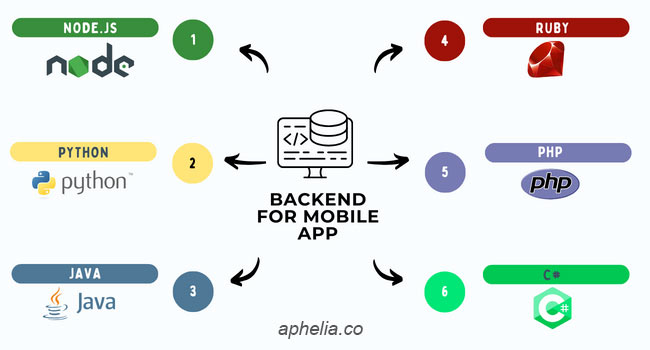
\includegraphics[width=0.75\textwidth]{images/backend_for_mobile_app.jpg}
        \caption{Một số công nghệ phát triển backend cho ứng dụng di động \cite{aphelia2023}.}
        \label{fig:fig1}
      \end{figure}
        \vspace{0.5em}
      
        Về cơ sở dữ liệu, có thể sử dụng các hệ quản trị quan hệ như MySQL hoặc PostgreSQL, tùy theo độ phức tạp của dữ liệu và yêu cầu về hiệu năng. MySQL phù hợp cho các ứng dụng cần tính ổn định cao, trong khi PostgreSQL cung cấp nhiều tính năng nâng cao hơn. Đối với các ứng dụng di động yêu cầu đồng bộ dữ liệu theo thời gian thực, Firebase Firestore là một lựa chọn phù hợp nhờ khả năng cập nhật nhanh và hỗ trợ tốt cho môi trường di động.
      
        \vspace{0.5em}
      
        Phía frontend và mobile, các framework như React Native, Flutter, Swift, và Kotlin là những lựa chọn phổ biến. React Native và Flutter hỗ trợ phát triển ứng dụng đa nền tảng, trong khi Swift và Kotlin là lựa chọn tối ưu cho phát triển ứng dụng gốc trên iOS và Android tương ứng.
      
        \vspace{0.5em}
      
        Cuối cùng, để tự động hóa quy trình triển khai và kiểm thử, các công cụ CI/CD như GitHub Actions hoặc Jenkins thường được tích hợp vào chu trình phát triển phần mềm. CI/CD là viết tắt của Continuous Integration và Continuous Deployment/Delivery, nghĩa là tích hợp liên tục và triển khai liên tục. Trong quy trình này, mã nguồn được kiểm tra, xây dựng và đưa lên môi trường thử nghiệm hoặc sản xuất một cách tự động, giúp phát hiện lỗi sớm và rút ngắn thời gian phát hành phần mềm.
      
   

\section{Lịch sử ngành lập trình di động}
\begin{flushleft}
  \hspace*{0.8cm}Ngành lập trình di động không xuất hiện một cách đột ngột, mà hình thành song song với sự phát triển của điện thoại di động qua từng thời kỳ. Từ những thiết bị to lớn, đắt đỏ và đơn chức năng, đến các smartphone hiện đại với khả năng xử lý mạnh mẽ và đa nhiệm, lập trình di động đã dần trở thành một lĩnh vực quan trọng trong ngành công nghệ thông tin. Việc hiểu rõ bối cảnh và các bước ngoặt trong lịch sử phát triển không chỉ giúp ta nhìn nhận đúng vai trò của lập trình di động, mà còn cho thấy những thách thức và cơ hội trong hành trình tạo ra các ứng dụng phục vụ hàng tỷ người dùng trên toàn cầu.
\end{flushleft}
% 2.1
\subsection{Tổng quan về lịch sử ngành lập trình di động}
\renewcommand{\labelitemi}{--}  

\begin{flushleft}
  \hspace*{0.8cm}Lập trình di động là một lĩnh vực đã phát triển song hành với sự tiến hóa của thiết bị di động trong suốt nhiều thập kỷ. Từ những năm 1990, khi các thiết bị cầm tay đầu tiên như Nokia và BlackBerry bắt đầu phổ biến, nhu cầu về các phần mềm cơ bản như lịch, máy tính và trò chơi đơn giản đã thúc đẩy sự ra đời của các nền tảng lập trình di động ban đầu. Những ứng dụng này chủ yếu được viết bằng ngôn ngữ C hoặc Java ME, giới hạn bởi phần cứng yếu và màn hình nhỏ.
\end{flushleft}

\begin{flushleft}
  \hspace*{0.8cm}Giai đoạn chuyển mình rõ rệt nhất của ngành bắt đầu từ năm 2007, khi Apple giới thiệu iPhone và hệ điều hành iOS. Sự xuất hiện của smartphone với màn hình cảm ứng, kết nối internet mạnh mẽ và kho ứng dụng trực tuyến đã tạo ra một bước ngoặt lớn. Ngay sau đó, Google ra mắt Android – một hệ điều hành mã nguồn mở, cho phép các nhà phát triển dễ dàng tạo ứng dụng và triển khai trên nhiều thiết bị khác nhau.
\end{flushleft}

\begin{flushleft}
  \hspace*{0.8cm}Từ năm 2010 đến nay, lập trình di động đã trở thành một trong những lĩnh vực sôi động nhất của ngành công nghệ thông tin. Các công cụ phát triển như Android Studio, Xcode, cùng với các framework đa nền tảng như React Native, Flutter hay Xamarin, đã giúp rút ngắn thời gian phát triển và mở rộng khả năng tiếp cận người dùng. Đồng thời, những xu hướng mới như trí tuệ nhân tạo (AI), thực tế tăng cường (AR), và Internet vạn vật (IoT) cũng được tích hợp ngày càng sâu vào các ứng dụng di động.
\end{flushleft}

\begin{flushleft}
  \hspace*{0.8cm}Có thể thấy, lịch sử ngành lập trình di động không chỉ phản ánh sự tiến bộ của công nghệ phần cứng và phần mềm, mà còn cho thấy vai trò ngày càng lớn của các ứng dụng trong đời sống hàng ngày. Hiểu rõ bối cảnh lịch sử này là cơ sở quan trọng để các nhà phát triển định hướng tương lai, lựa chọn công cụ phù hợp, và xây dựng các giải pháp sáng tạo đáp ứng nhu cầu người dùng hiện đại.
\end{flushleft}

% 2.2
\subsection{Một số thiết kế của điện thoại di động qua từng thời kỳ}
\renewcommand{\labelitemi}{--}    
    \begin{flushleft}
        \hspace*{0.8cm}Vào những năm 1980, những chiếc điện thoại di động đầu tiên ra đời với thiết kế to, nặng và thường phải mang theo như một chiếc túi xách. Các thiết bị này chủ yếu được sử dụng để nghe và gọi, không có màn hình hiển thị hoặc giao diện tương tác như hiện nay. Lúc này, khái niệm về lập trình di động vẫn chưa xuất hiện vì các thiết bị không hỗ trợ cài đặt thêm phần mềm.
    \end{flushleft}

    \begin{flushleft}
      \hspace*{0.8cm}Đến thập niên 1990, cùng với sự phát triển của công nghệ vi mạch và màn hình LCD, điện thoại di động bắt đầu trở nên nhỏ gọn và phổ biến hơn. Các dòng máy như Nokia 3210 hay Motorola StarTAC không chỉ hỗ trợ gọi điện và nhắn tin, mà còn tích hợp một số ứng dụng đơn giản như đồng hồ báo thức, lịch và trò chơi Snake. Đây là thời kỳ lập trình di động bắt đầu hình thành, chủ yếu dưới dạng các phần mềm nhúng hoặc ứng dụng đơn giản viết bằng ngôn ngữ C hoặc Java ME.
  \end{flushleft}

  \begin{flushleft}
    \hspace*{0.8cm}Giai đoạn tiếp theo bắt đầu từ năm 2007, khi Apple ra mắt iPhone – một thiết bị đánh dấu kỷ nguyên mới của điện thoại thông minh. Với màn hình cảm ứng đa điểm, hiệu năng mạnh mẽ và khả năng kết nối internet, iPhone đã thay đổi hoàn toàn cách người dùng tương tác với thiết bị di động. Sự ra đời của App Store vào năm 2008 đã mở ra một thị trường ứng dụng sôi động, thúc đẩy sự phát triển mạnh mẽ của lập trình di động. Gần như song song, Google cũng phát triển Android – hệ điều hành mã nguồn mở, cho phép các nhà sản xuất và lập trình viên tự do phát triển ứng dụng và tùy biến theo nhu cầu.
\end{flushleft}

\begin{flushleft}
  \hspace*{0.8cm}Từ năm 2010 đến nay, thiết bị di động đã đạt được những bước tiến vượt bậc về hiệu năng, độ phân giải màn hình, dung lượng pin và khả năng xử lý đa nhiệm. Đồng thời, các công nghệ mới như trí tuệ nhân tạo (AI), thực tế ảo (VR), thực tế tăng cường (AR), và cảm biến sinh trắc học cũng được tích hợp ngày càng sâu vào thiết bị. Bên cạnh đó, sự xuất hiện của các nền tảng phát triển đa nền tảng như React Native, Flutter, và Xamarin đã tạo điều kiện thuận lợi cho các nhà phát triển viết ứng dụng một lần và triển khai trên cả iOS lẫn Android.
\end{flushleft}

\begin{flushleft}
  \hspace*{0.8cm}Có thể thấy, thiết bị di động không ngừng được cải tiến cả về phần cứng lẫn phần mềm. Từ một công cụ liên lạc đơn giản, chúng đã trở thành trung tâm của mọi hoạt động số hóa trong đời sống hiện đại – từ học tập, làm việc, giải trí cho đến quản lý tài chính cá nhân. Quá trình phát triển qua các giai đoạn này không chỉ mở ra nhiều cơ hội cho lập trình viên, mà còn đặt ra những thách thức mới về hiệu suất, bảo mật và trải nghiệm người dùng.
\end{flushleft}

% 2.3
\subsection{Motorola DynaTAC 8000X – Bước ngoặt đầu tiên của điện thoại di động}
\renewcommand{\labelitemi}{--}    
\begin{flushleft}
    \hspace*{0.8cm}Motorola DynaTAC 8000X, được giới thiệu vào năm 1983, là chiếc điện thoại di động thương mại đầu tiên trên thế giới. Thiết bị này đã đánh dấu một bước ngoặt quan trọng trong ngành viễn thông toàn cầu khi lần đầu tiên mang lại khả năng liên lạc di động thực sự cho người dùng cá nhân. Với hình dáng to lớn và trọng lượng nặng, DynaTAC vẫn nhanh chóng trở thành biểu tượng công nghệ của thời đại, đặt nền móng cho sự hình thành và phát triển sau này của các thiết bị di động thông minh cũng như ngành lập trình ứng dụng di động.~\cite{motorola1983}
\end{flushleft}

\begin{flushleft}
  \hspace*{0.8cm}DynaTAC 8000X sở hữu thiết kế nổi bật theo phong cách công nghiệp, với kích thước khoảng 33 x 4.4 x 8.9 cm và trọng lượng lên đến 1.1 kg. Người dùng cần sử dụng cả hai tay để thao tác, khiến nó được gọi với biệt danh quen thuộc là “brick phone” – điện thoại cục gạch. Đây là minh chứng rõ rệt cho giai đoạn khởi đầu của công nghệ di động, khi tính cơ động vẫn còn là một khái niệm tương đối.
\end{flushleft}

\begin{flushleft}
  \hspace*{0.8cm}Về mặt kinh tế, thiết bị này là một sản phẩm xa xỉ. Với mức giá lên tới \$3,995 vào năm 1983 (tương đương hơn \$10,000 hiện nay sau điều chỉnh lạm phát), DynaTAC chỉ phù hợp với tầng lớp thượng lưu hoặc những người có nhu cầu đặc biệt. Không chỉ đắt đỏ về giá mua, người dùng còn phải trả thêm chi phí thuê bao hàng tháng và phí gọi tính theo phút – làm cho việc sử dụng thiết bị trở thành một khoản đầu tư lớn về tài chính.
\end{flushleft}

\begin{flushleft}
  \hspace*{0.8cm}Về mặt kỹ thuật, DynaTAC không sở hữu màn hình màu, cảm ứng hay các chức năng nâng cao. Thiết bị chỉ phục vụ chức năng cơ bản là thực hiện và nhận cuộc gọi. Tuy nhiên, chính việc đưa công nghệ viễn thông ra khỏi không gian cố định – như điện thoại bàn – đã mở ra một thời kỳ hoàn toàn mới, trong đó việc giao tiếp trở nên linh hoạt hơn bao giờ hết. Đó là tiền đề quan trọng để những công nghệ di động sau này phát triển mạnh mẽ hơn.
\end{flushleft}

\begin{flushleft}
  \hspace*{0.8cm}Tuy không hỗ trợ cài đặt phần mềm hay ứng dụng, DynaTAC vẫn có vai trò đặc biệt trong lịch sử lập trình di động. Sự xuất hiện của nó đã cho thấy tiềm năng thương mại rất lớn của các thiết bị cầm tay, từ đó thúc đẩy các nhà sản xuất phần cứng và kỹ sư viễn thông đầu tư vào nghiên cứu, phát triển hệ điều hành và nền tảng phần mềm cho thiết bị di động. Nhu cầu mở rộng chức năng thiết bị đã đặt nền móng cho việc phát triển các ứng dụng nhúng đầu tiên và các hệ điều hành cơ bản dành riêng cho di động.
\end{flushleft}

\begin{flushleft}
  \hspace*{0.8cm}Nhìn một cách tổng thể, DynaTAC 8000X không chỉ là thiết bị điện thoại đầu tiên mà còn là biểu tượng khởi đầu của một ngành công nghiệp đầy tiềm năng. Mặc dù giới hạn về công nghệ và chức năng, sự thành công thương mại của nó đã truyền cảm hứng cho hàng loạt phát minh sau này – từ điện thoại thông minh cho tới hệ sinh thái lập trình ứng dụng di động đa dạng và phong phú như hiện nay.
\end{flushleft}

% 2.4
\subsection{Từ “cục gạch” đến trải nghiệm người dùng hiện đại}
\renewcommand{\labelitemi}{--}    
    \begin{flushleft}
        \hspace*{0.8cm}Sau khi điện thoại di động ra đời vào thập niên 1980, công nghệ đã không ngừng tiến hóa để biến những thiết bị vốn to lớn, nặng nề và đắt đỏ thành các sản phẩm nhỏ gọn, tiện lợi và phổ biến trong đời sống hàng ngày. Quá trình thu nhỏ phần cứng đi kèm với việc mở rộng khả năng xử lý và kết nối đã biến điện thoại di động từ một công cụ liên lạc thành một nền tảng công nghệ mạnh mẽ. Trong bối cảnh đó, trải nghiệm người dùng (User Experience – UX) dần trở thành một yếu tố trọng tâm, không chỉ trong thiết kế phần cứng mà còn trong quá trình phát triển phần mềm ứng dụng.
    \end{flushleft}

    \begin{flushleft}
      \hspace*{0.8cm}Sự phát triển của UX trên thiết bị di động gắn liền với sự thay đổi trong hành vi và kỳ vọng của người dùng. Ban đầu, người dùng điện thoại di động chủ yếu mong muốn một thiết bị có thể thực hiện cuộc gọi ổn định và dễ sử dụng. Tuy nhiên, khi điện thoại trở nên phổ biến và chuyển mình thành điện thoại thông minh, người dùng bắt đầu kỳ vọng nhiều hơn: giao diện phải trực quan, tốc độ xử lý nhanh, thao tác mượt mà và trải nghiệm tổng thể phải liền mạch. Chính sự thay đổi về nhận thức và nhu cầu này đã thúc đẩy ngành lập trình di động phải chuyển hướng từ lập trình chức năng đơn thuần sang thiết kế lấy người dùng làm trung tâm.
    \end{flushleft}

    \begin{flushleft}
      \hspace*{0.8cm}Việc điện thoại trở nên dễ tiếp cận hơn là một trong những yếu tố khiến UX trở thành một vấn đề cốt lõi. Nếu như những chiếc điện thoại đầu tiên có giá hàng nghìn đô la và chỉ phục vụ giới doanh nhân, thì ngày nay, người dùng ở mọi độ tuổi và tầng lớp xã hội đều có thể sở hữu ít nhất một thiết bị di động. Khi số lượng người dùng tăng lên, sự đa dạng về nhu cầu, trình độ công nghệ và thị hiếu sử dụng cũng trở nên phong phú hơn. Điều này tạo ra áp lực lớn đối với các nhà phát triển phần mềm, buộc họ phải tạo ra những sản phẩm vừa đơn giản, dễ dùng, vừa đầy đủ chức năng và mang lại cảm giác sử dụng thoải mái.
  \end{flushleft}

  \begin{flushleft}
    \hspace*{0.8cm}Bên cạnh sự thay đổi của người dùng, sự tiến bộ nhanh chóng của phần cứng cũng là một yếu tố không thể bỏ qua. Các thiết bị hiện đại sở hữu màn hình độ phân giải cao, cảm ứng đa điểm, bộ xử lý mạnh, RAM lớn và pin dung lượng cao. Những tiến bộ này mở ra cơ hội cho các nhà phát triển phần mềm thiết kế giao diện ngày càng sinh động, đẹp mắt và tương tác tốt hơn. Nếu như trước đây ứng dụng di động chỉ có thể hiển thị văn bản đơn giản hoặc hình ảnh tĩnh, thì hiện nay, chúng có thể tích hợp video, hiệu ứng chuyển động, phản hồi xúc giác và thậm chí cả trí tuệ nhân tạo để cá nhân hóa trải nghiệm người dùng.
  \end{flushleft}

  \begin{flushleft}
    \hspace*{0.8cm}Sự thay đổi lớn cũng diễn ra trong vai trò của các nhà sản xuất thiết bị di động. Trong giai đoạn đầu, các nhà sản xuất phần cứng thường là những người duy nhất phát triển phần mềm cho thiết bị của họ, từ giao diện người dùng cho đến các chức năng cơ bản. Tuy nhiên, mô hình này nhanh chóng bộc lộ hạn chế khi không thể đáp ứng kịp tốc độ thay đổi của thị trường và nhu cầu người dùng. Đồng thời, các nhà sản xuất cũng không sẵn sàng chia sẻ chi tiết về phần cứng của họ vì lý do bảo mật và cạnh tranh, khiến cho bên thứ ba rất khó tiếp cận và phát triển phần mềm.
  \end{flushleft}

  \begin{flushleft}
    \hspace*{0.8cm}Chính sự bất cập đó đã làm nảy sinh một nhu cầu mới: cần có một lớp trung gian – hay chính xác hơn là một chuẩn kỹ thuật – giúp kết nối phần mềm với phần cứng một cách hiệu quả và an toàn. Các API (Application Programming Interface), SDK (Software Development Kit) và hệ điều hành di động như iOS hay Android đã ra đời nhằm mục đích đó. Chúng đóng vai trò là cầu nối giữa nhà sản xuất thiết bị và cộng đồng lập trình viên, giúp quá trình phát triển phần mềm trở nên dễ dàng hơn mà không cần phải hiểu sâu về kiến trúc phần cứng.
  \end{flushleft}

  \begin{flushleft}
    \hspace*{0.8cm}Một trong những giải pháp mở đầu cho quá trình này là việc sử dụng trình duyệt web di động như một nền tảng để triển khai ứng dụng. Thay vì phát triển phần mềm cài đặt riêng biệt, các lập trình viên bắt đầu tối ưu hóa trang web để hoạt động tốt trên điện thoại. Từ đó, khái niệm “ứng dụng web di động” ra đời, đóng vai trò như bước chuyển tiếp giữa trình duyệt truyền thống và ứng dụng gốc (native app). Những trải nghiệm đầu tiên trên nền tảng web đã đặt nền móng cho việc hình thành tư duy thiết kế giao diện người dùng hiện đại.
  \end{flushleft}

  \begin{flushleft}
    \hspace*{0.8cm}Nhìn chung, sự phát triển của UX trên thiết bị di động không chỉ phản ánh tiến bộ của công nghệ mà còn cho thấy mối liên kết chặt chẽ giữa phần cứng, phần mềm và hành vi người dùng. Việc đặt người dùng làm trung tâm không chỉ là xu hướng tạm thời mà đã trở thành triết lý phát triển cốt lõi trong ngành lập trình di động hiện đại. Từ “cục gạch” thô sơ ngày xưa đến những chiếc điện thoại tinh xảo hiện nay, trải nghiệm người dùng chính là yếu tố quyết định sự thành bại của một sản phẩm trong thời đại số.
  \end{flushleft}

% 2.5
\subsection{Chuẩn WAP – Khởi đầu cho trình duyệt web trên di động}
\renewcommand{\labelitemi}{--}    
\begin{flushleft}
  \hspace*{0.8cm}Trong những năm cuối thập niên 1990 và đầu những năm 2000, khi điện thoại di động bắt đầu được sử dụng rộng rãi trên toàn cầu, nhu cầu truy cập thông tin mọi lúc mọi nơi cũng trở nên cấp thiết. Tuy nhiên, hạ tầng mạng di động ở thời kỳ này lại chưa đủ phát triển: tốc độ kết nối rất chậm, băng thông hạn chế, và độ ổn định thấp. Vì vậy, việc sử dụng các trang web HTML tiêu chuẩn như trên máy tính là điều gần như không khả thi trên thiết bị di động lúc bấy giờ.
  \end{flushleft}
  
  \begin{flushleft}
  \hspace*{0.8cm}Để giải quyết những hạn chế đó, chuẩn WAP – Wireless Application Protocol đã được ra đời như một giải pháp trung gian nhằm hiện thực hóa giấc mơ duyệt web trên thiết bị di động. WAP là một giao thức truyền thông được thiết kế đặc biệt cho môi trường mạng không dây với mục tiêu tạo điều kiện cho các thiết bị di động có thể truy cập, nhận và hiển thị dữ liệu từ các máy chủ web.
  \end{flushleft}
  
  \begin{flushleft}
  \hspace*{0.8cm}Khác với giao thức HTTP vốn được xây dựng cho các máy tính kết nối mạng ổn định và tốc độ cao, WAP được ví như một “phiên bản rút gọn” của HTTP, tối ưu hóa cho việc vận hành trên các thiết bị có tài nguyên phần cứng hạn chế và kết nối mạng chậm như 2G hay GPRS. Nhờ vậy, dù rất đơn giản và sơ khai, WAP đã đóng vai trò như chiếc cầu nối giữa thế giới web truyền thống và thiết bị di động.
  \end{flushleft}
  
  \begin{flushleft}
  \hspace*{0.8cm}Một trong những yếu tố then chốt làm nên hiệu quả của WAP chính là ngôn ngữ đánh dấu WML (Wireless Markup Language). Thay vì sử dụng HTML, vốn quá nặng và phức tạp với các thiết bị di động thời bấy giờ, WML được thiết kế nhẹ hơn nhiều, loại bỏ các yếu tố đồ họa và định dạng phức tạp. Cú pháp của WML khá giống HTML nhưng bị giới hạn về số lượng thẻ và khả năng tương tác. Điều này cho phép hiển thị nội dung văn bản đơn giản như tiêu đề, đoạn văn, và các liên kết mà vẫn đảm bảo tốc độ tải nhanh và khả năng tương thích với phần cứng yếu.
  \end{flushleft}
  
  \begin{flushleft}
  \hspace*{0.8cm}Thêm vào đó, kiến trúc của WAP được xây dựng xoay quanh nguyên tắc tối ưu cho mạng yếu, nhằm giảm thiểu tối đa dữ liệu cần truyền và yêu cầu xử lý phức tạp. Nhờ đó, các thiết bị di động có thể tải và hiển thị nội dung một cách hiệu quả hơn, dù đang hoạt động trong điều kiện mạng không ổn định và băng thông hạn chế.
  \end{flushleft}
  
  \begin{flushleft}
  \hspace*{0.8cm}Trong thời kỳ đầu, nhiều tổ chức và hãng thông tấn đã nhanh chóng nhận ra tiềm năng của WAP và bắt đầu phát triển các phiên bản website hỗ trợ giao thức này. CNN là một trong những đơn vị tiên phong, cung cấp nội dung tin tức thời sự cho người dùng di động thông qua nền tảng WAP. Tương tự, ESPN cũng phát triển phiên bản WAP nhằm cập nhật tỉ số thể thao và thông tin thi đấu cho khán giả thường xuyên di chuyển.
  \end{flushleft}
  
  \begin{flushleft}
  \hspace*{0.8cm}Những ví dụ kể trên là minh chứng rõ ràng cho việc các nhà phát triển ứng dụng web đã bắt đầu chú trọng đến nền tảng di động, dù với rất nhiều giới hạn kỹ thuật so với web truyền thống trên máy tính. Tuy vậy, chính những nỗ lực này đã mở ra một hướng đi mới cho lĩnh vực phát triển ứng dụng – hướng đi mà sau này sẽ trở thành một trụ cột quan trọng trong ngành công nghệ.
  \end{flushleft}
  
  \begin{flushleft}
  \hspace*{0.8cm}Xét về mặt lịch sử và ý nghĩa đối với lập trình di động, WAP có thể được xem là cột mốc đánh dấu sự khởi đầu của khái niệm "ứng dụng web di động". Nhờ vào chuẩn này, các lập trình viên thời kỳ đầu đã có môi trường và công cụ để bắt đầu phát triển nội dung dành riêng cho điện thoại di động, dù chỉ ở mức rất cơ bản.
  \end{flushleft}
  
  \begin{flushleft}
  \hspace*{0.8cm}Không những thế, việc áp dụng WAP còn giúp định hình tư duy thiết kế ứng dụng tối giản, ưu tiên tốc độ và hiệu năng – một nguyên tắc vẫn còn giá trị trong phát triển ứng dụng di động hiện đại. Đồng thời, nó cũng mở ra kỷ nguyên mà điện thoại không chỉ là thiết bị nghe gọi, mà còn là cổng kết nối đến thế giới thông tin số – nơi người dùng có thể cập nhật tin tức, tra cứu thông tin, hay tương tác với nội dung web ở bất cứ đâu.
  \end{flushleft}

% 2.6
\subsection{Sự phát triển của thanh toán di động và bước ngoặt trong lập trình ứng dụng}
\renewcommand{\labelitemi}{--}

\begin{flushleft}
\hspace*{0.8cm}Khi điện thoại di động dần trở thành một phần thiết yếu trong đời sống hàng ngày, nhu cầu không chỉ dừng lại ở liên lạc mà còn mở rộng sang các tiện ích phục vụ tiêu dùng và giải trí. Trong quá trình phát triển đó, một yếu tố có vai trò đặc biệt quan trọng trong việc thúc đẩy sự bùng nổ của ứng dụng di động chính là khả năng thanh toán ngay trên thiết bị.
\end{flushleft}

\begin{flushleft}
\hspace*{0.8cm}Trong những ngày đầu, hình thức thanh toán thông qua SMS (Short Message Service) được xem là giải pháp khả thi nhất, bởi vì hầu hết các điện thoại di động đều hỗ trợ gửi và nhận tin nhắn. Với mô hình này, người dùng chỉ cần gửi tin nhắn đến một đầu số dịch vụ như 8xxx hoặc 6xxx để đổi lại các nội dung số như nhạc chuông, hình nền, hình động hay truyện cười. Khoản phí của tin nhắn này cao hơn nhiều so với tin nhắn thông thường và được tính trực tiếp vào tài khoản di động.
\end{flushleft}

\begin{flushleft}
\hspace*{0.8cm}Những tin nhắn dạng này được gọi là VAS – Value Added Services (dịch vụ giá trị gia tăng), và chính chúng đã đặt nền móng cho mô hình kinh doanh nội dung số trên nền tảng di động. Đây cũng là lần đầu tiên mà lập trình viên có thể kiếm tiền thông qua các ứng dụng hoặc nội dung do họ xây dựng, dù vẫn còn ở dạng rất đơn giản.
\end{flushleft}

\begin{flushleft}
\hspace*{0.8cm}Khi điện thoại phát triển và người dùng ngày càng quen với việc tiêu dùng nội dung số, nhiều hình thức thanh toán khác cũng nhanh chóng ra đời để thay thế hoặc bổ sung cho SMS, tạo điều kiện mở rộng mô hình kinh doanh ứng dụng. Một trong số đó là thẻ cào điện thoại, cho phép người dùng nạp tiền vào tài khoản chính rồi sử dụng số dư này để mua vật phẩm hoặc dịch vụ trong game và ứng dụng.
\end{flushleft}

\begin{flushleft}
\hspace*{0.8cm}Tiếp theo là web charging, một hình thức thanh toán hiện đại hơn, cho phép người dùng mua nội dung trực tiếp trên website hoặc ứng dụng mà không cần can thiệp thủ công. Khi người dùng chọn một dịch vụ trên trình duyệt hoặc trong app, hệ thống sẽ tự động trừ tiền vào tài khoản di động mà không yêu cầu xác nhận nhiều bước. Dù còn hạn chế và dễ phát sinh lỗi, web charging đã cho thấy tiềm năng to lớn của thương mại điện tử di động trong tương lai.
\end{flushleft}

\begin{flushleft}
\hspace*{0.8cm}Mặc dù các hình thức thanh toán kể trên còn đơn giản và chưa được bảo mật cao, nhưng chính chúng đã mở ra cánh cửa đầu tiên cho khái niệm “thanh toán di động”. Từ đó, lập trình viên không chỉ viết ứng dụng phục vụ giải trí mà còn có cơ hội tạo ra giá trị kinh tế thực sự, khuyến khích việc đầu tư bài bản vào thiết kế, trải nghiệm người dùng và chiến lược kiếm tiền.
\end{flushleft}

\begin{flushleft}
\hspace*{0.8cm}Song song với sự phát triển của các mô hình thanh toán, ngành lập trình di động cũng chứng kiến một bước chuyển mình mạnh mẽ. Khi người dùng tăng trưởng nhanh chóng và nhu cầu sử dụng di động vượt xa kỳ vọng, các công ty công nghệ lớn như Apple, Google, và sau này là Samsung, Huawei đã chính thức bước vào cuộc chơi với các hệ điều hành và nền tảng ứng dụng riêng biệt.
\end{flushleft}

\begin{flushleft}
\hspace*{0.8cm}Trước giai đoạn này, lập trình di động vẫn chủ yếu dựa vào nền tảng J2ME (Java 2 Micro Edition) – một môi trường phát triển cực kỳ rối rắm. Các lập trình viên phải đối mặt với hàng loạt thách thức: mỗi dòng điện thoại lại có độ phân giải khác nhau, hệ thống phím bấm không đồng nhất, dung lượng bộ nhớ thấp và phần cứng yếu. Công cụ hỗ trợ thì thiếu thốn, giao diện đơn điệu và không có khả năng tái sử dụng mã nguồn.
\end{flushleft}

\begin{flushleft}
\hspace*{0.8cm}Chỉ đến khi phần cứng của thiết bị di động có bước tiến vượt bậc – với màn hình cảm ứng lớn, bộ xử lý mạnh, bộ nhớ RAM dồi dào, cùng lúc đó là sự xuất hiện của iOS (Swift/Objective-C) và Android (Java/Kotlin) – lập trình viên mới thực sự có cơ hội khai phá sức mạnh của nền tảng di động một cách toàn diện. Giao diện đẹp hơn, tốc độ xử lý nhanh hơn và đặc biệt là hệ sinh thái phát triển (SDK, IDE, kho ứng dụng) đầy đủ và nhất quán, đã tạo ra một cuộc cách mạng trong phát triển ứng dụng.
\end{flushleft}

% 2.7
\subsection{Thị trường di động trên toàn thế giới}
\renewcommand{\labelitemi}{--}    
\begin{flushleft}
  \hspace*{0.8cm}Trước năm 2010, khi khái niệm “smartphone” còn khá mới mẻ với phần lớn người dùng, thị trường điện thoại di động toàn cầu vẫn được dẫn dắt bởi những thương hiệu gắn liền với sự bền bỉ, phổ thông và dễ sử dụng. Nổi bật trong số đó, không ai khác chính là Nokia – “ông vua” không ngai của thời kỳ tiền smartphone.
  \end{flushleft}
  
  \begin{flushleft}
  \hspace*{0.8cm}Nokia đã từng bước định hình trải nghiệm di động cho hàng triệu người dùng trên toàn thế giới, từ những chiếc điện thoại đen trắng cơ bản đến các dòng máy màu, hỗ trợ nhạc chuông đa âm, chơi game Java, cài đặt phần mềm và chụp ảnh. Những model như Nokia 1100, 6300, N70, N95 không chỉ phổ biến mà còn trở thành biểu tượng của một thời kỳ công nghệ giản đơn mà hiệu quả.
  \end{flushleft}
  
  \begin{flushleft}
  \hspace*{0.8cm}Tại Việt Nam, Nokia chiếm trọn niềm tin của người dùng nhờ thiết kế chắc chắn, pin “trâu”, giá thành hợp lý và khả năng hoạt động bền bỉ trong nhiều năm. Sự phổ biến của thương hiệu này mạnh đến mức tên “Nokia” từng được dùng để gọi chung cho bất kỳ chiếc điện thoại nào, dù có thể đó là sản phẩm của hãng khác.
  \end{flushleft}
  
  \begin{flushleft}
  \hspace*{0.8cm}Song song với Nokia, các hãng như Blackberry, Sony Ericsson, Samsung, HTC cũng không ngừng nỗ lực chiếm lĩnh thị phần bằng cách phát triển các hệ điều hành riêng biệt hoặc hợp tác với bên thứ ba để tạo ra sự khác biệt. Một số nền tảng phổ biến lúc bấy giờ gồm:
  \begin{itemize}
  \item Symbian (Nokia)
  \item Blackberry OS (Blackberry)
  \item Windows Mobile, Windows CE (Microsoft)
  \item Palm OS, Linux Mobile, Bada OS (Samsung)
  \end{itemize}
  \end{flushleft}
  
  \begin{flushleft}
  \hspace*{0.8cm}Tuy nhiên, một điểm yếu chung của tất cả các hệ điều hành kể trên chính là sự thiếu thống nhất và không thân thiện với lập trình viên. Mỗi hệ điều hành lại có giao diện riêng, API riêng, ngôn ngữ lập trình và tài liệu khác nhau – gây ra vô vàn khó khăn cho nhà phát triển:
  \begin{itemize}
  \item Trải nghiệm người dùng không đồng đều, giao diện không thống nhất.
  \item Bộ công cụ phát triển (SDK) còn sơ khai, thiếu tính năng và khó tiếp cận.
  \item Không có kho ứng dụng tập trung, dẫn đến việc phân phối phần mềm cực kỳ phức tạp.
  \item[]Điều này khiến phần lớn lập trình viên thời điểm đó vẫn còn thờ ơ hoặc làm việc theo kiểu "cho có", bởi chưa có hệ sinh thái đủ hấp dẫn để đầu tư nghiêm túc.
  \end{itemize}
  \end{flushleft}
  
  \begin{flushleft}
  \hspace*{0.8cm}Mọi thứ chỉ thật sự thay đổi khi Apple chính thức ra mắt iPhone vào năm 2007. Thiết bị này không chỉ là một chiếc điện thoại thông minh đầu tiên theo đúng nghĩa hiện đại, mà còn là bước ngoặt vĩ đại của toàn ngành công nghiệp di động.
  \end{flushleft}
  
  \begin{flushleft}
  \hspace*{0.8cm}Với màn hình cảm ứng đa điểm, thiết kế tinh tế không dùng bàn phím vật lý, hiệu năng mạnh mẽ và hệ điều hành ổn định, iPhone đã đặt ra một chuẩn mực mới cho smartphone. Tuy nhiên, cú hích lớn nhất chỉ đến vào năm 2008, khi App Store chính thức ra đời – nền tảng phân phối ứng dụng tập trung đầu tiên trong lịch sử di động.
  \end{flushleft}
  
  \begin{flushleft}
  \hspace*{0.8cm}App Store không chỉ giúp người dùng dễ dàng tìm kiếm và cài đặt phần mềm, mà còn mở ra cơ hội kinh doanh ứng dụng chuyên nghiệp cho lập trình viên trên toàn thế giới. Với một bộ công cụ phát triển mạnh mẽ, tài liệu hướng dẫn đầy đủ và cộng đồng sôi nổi, iOS SDK đã biến lập trình di động từ một công việc khó khăn, mơ hồ thành một ngành công nghiệp sáng tạo thực thụ.
  \end{flushleft}
  
  \begin{flushleft}
  \hspace*{0.8cm}Kể từ đây, lập trình ứng dụng di động bước sang một kỷ nguyên mới, nơi trải nghiệm người dùng, hiệu năng và hệ sinh thái phát triển đóng vai trò trung tâm. Cuộc đua giữa các nền tảng như iOS và Android cũng bắt đầu, tạo nên một trong những giai đoạn sôi động nhất trong lịch sử công nghệ di động.
  \end{flushleft}

% 2.8
\subsection{Thị trường và sự cạnh tranh trong ngành lập trình di động}
\renewcommand{\labelitemi}{--}    
    \begin{flushleft}
        \hspace*{0.8cm}Khi thị trường thiết bị di động bắt đầu bùng nổ vào đầu thập niên 2010, ba ông lớn công nghệ là Microsoft, Apple và Google đã nhanh chóng bước vào một cuộc cạnh tranh gay gắt nhằm chiếm lĩnh thị phần trong cả phần cứng, hệ điều hành và hệ sinh thái ứng dụng. Mỗi công ty lựa chọn một chiến lược phát triển riêng biệt, qua đó không chỉ định hình diện mạo ngành công nghiệp di động mà còn tác động sâu rộng đến cách thức phát triển ứng dụng di động sau này.
    \end{flushleft}

    \begin{flushleft}
      \hspace*{0.8cm}Trong ba ông lớn, Microsoft là cái tên bước vào cuộc chơi di động với nhiều tham vọng nhưng lại chậm chân. Sau khi nhận ra xu thế bùng nổ của smartphone, Microsoft đã tiến hành một thương vụ lớn vào năm 2013: mua lại bộ phận thiết bị và dịch vụ của Nokia với kỳ vọng tạo ra một hệ sinh thái Windows toàn diện, thống nhất từ máy tính, máy tính bảng đến điện thoại. Triết lý phát triển "Windows Universal Platform" (UWP) – một ứng dụng chạy được trên mọi thiết bị – là nỗ lực nhằm tối ưu trải nghiệm lập trình viên và người dùng. Tuy nhiên, Windows Phone lại xuất hiện quá muộn so với iOS và Android. Kho ứng dụng nghèo nàn, cộng đồng lập trình viên thiếu mặn mà, và mặc dù hệ điều hành này có trải nghiệm mượt mà, nhưng lại thiếu linh hoạt và không thể cá nhân hóa sâu. Kết quả, Windows Phone dần bị người dùng quay lưng và cuối cùng bị khai tử, để lại một bài học sâu sắc về tầm quan trọng của thời điểm gia nhập thị trường và sự linh hoạt trong thích nghi với xu thế công nghệ.
    \end{flushleft}

    \begin{flushleft}
      \hspace*{0.8cm}Ngược lại với Microsoft, Apple là công ty dẫn đầu trong cả trải nghiệm người dùng lẫn xây dựng hệ sinh thái khép kín. Với triết lý thiết kế "từ trong ra ngoài" – nghĩa là kiểm soát cả phần cứng và phần mềm – Apple tạo ra sự đồng bộ, ổn định và an toàn cao cho các thiết bị của mình. iPhone nổi bật với thiết kế tinh tế, hiệu năng mượt mà; hệ điều hành iOS ít lỗi và có tính bảo mật cao; App Store được quản lý chặt chẽ, đảm bảo chất lượng ứng dụng. Đồng thời, Apple luôn chú trọng đến việc hỗ trợ lập trình viên thông qua các công cụ chuyên nghiệp như Xcode, ngôn ngữ Swift và các framework như UIKit hay SwiftUI. Sự nhất quán này giúp Apple duy trì vị thế hàng đầu trong phân khúc smartphone cao cấp và sở hữu lượng người dùng trung thành cao bậc nhất thế giới.
    \end{flushleft}

    \begin{flushleft}
      \hspace*{0.8cm}Về phía Google, chiến lược phát triển của họ xoay quanh triết lý mã nguồn mở, với Android là trung tâm của hệ sinh thái di động. Thay vì sản xuất phần cứng đại trà như Apple, Google phát triển Android như một nền tảng mở, cho phép các nhà sản xuất như Samsung, Xiaomi, Oppo hay Huawei tùy biến và tích hợp hệ điều hành này vào thiết bị của họ. Cách tiếp cận này giúp Android nhanh chóng chiếm lĩnh thị phần toàn cầu. Ban đầu, Android bị phê phán vì tính phân mảnh và kém ổn định, nhưng theo thời gian, Google đã liên tục cải tiến hệ điều hành qua từng phiên bản, siết chặt tiêu chuẩn chất lượng trên Google Play và giới thiệu dòng thiết bị Pixel nhằm kiểm soát tốt hơn trải nghiệm người dùng. Nhờ vào sức mạnh về dữ liệu, trí tuệ nhân tạo và mạng lưới dịch vụ (Gmail, Maps, YouTube...), Google vẫn giữ vững vị thế là trụ cột của ngành di động hiện đại.
    \end{flushleft}

    \begin{flushleft}
      \hspace*{0.8cm}Sự cạnh tranh giữa Microsoft, Apple và Google – ba công ty với ba con đường phát triển khác nhau – không chỉ thúc đẩy đổi mới công nghệ mà còn tạo ra một hệ sinh thái lập trình di động phong phú, đa dạng và không ngừng phát triển. Chính sự đối đầu chiến lược này đã đặt nền móng cho những xu hướng lập trình đa nền tảng ngày nay.
    \end{flushleft}

% 2.9
\subsection{Hai hệ điều hành phổ biến nhất ngày nay: iOS và Android.}
\renewcommand{\labelitemi}{--}   
\begin{flushleft}
  \hspace*{0.8cm}Trong thị trường thiết bị di động hiện nay, iOS và Android là hai hệ điều hành chiếm lĩnh tuyệt đối, đồng thời là nền tảng chủ đạo cho việc phát triển ứng dụng di động trên toàn cầu. Mỗi hệ điều hành mang trong mình triết lý thiết kế, kiến trúc kỹ thuật và hệ sinh thái lập trình riêng, qua đó ảnh hưởng mạnh mẽ đến lựa chọn công cụ và quy trình làm việc của lập trình viên.
\end{flushleft}
    \begin{flushleft}
        \hspace*{0.8cm}iOS là hệ điều hành được phát triển độc quyền bởi Apple, chủ yếu sử dụng trên các thiết bị như iPhone, iPad và iPod Touch. Đặc điểm nổi bật của iOS là sự ổn định, hiệu suất cao và mức độ bảo mật nghiêm ngặt, được đảm bảo bởi quy trình kiểm duyệt ứng dụng chặt chẽ trên App Store. Về mặt lập trình, trước đây iOS sử dụng Objective-C, nhưng kể từ năm 2014, ngôn ngữ Swift – hiện đại, dễ học và tối ưu hóa hiệu năng – đã dần thay thế và trở thành ngôn ngữ chính trong phát triển iOS. Các công cụ hỗ trợ như Xcode đóng vai trò trung tâm trong quá trình phát triển, với khả năng mô phỏng, kiểm thử và tối ưu hóa ứng dụng. Ngoài ra, Apple cung cấp nhiều framework mạnh mẽ như UIKit và SwiftUI để xây dựng giao diện người dùng một cách linh hoạt. Tuy nhiên, do hệ sinh thái đóng, lập trình iOS thường phụ thuộc hoàn toàn vào công cụ và quy định của Apple.
    \end{flushleft}

    \begin{flushleft}
      \hspace*{0.8cm}Android, trái lại, là một hệ điều hành mã nguồn mở do Google phát triển, dựa trên nền tảng Linux. Sự cởi mở trong kiến trúc giúp Android được sử dụng trên hàng trăm thương hiệu thiết bị khác nhau như Samsung, Sony, Xiaomi, hay Oppo, từ đó tạo ra một thị trường đa dạng và cạnh tranh mạnh mẽ. Về ngôn ngữ lập trình, Android ban đầu sử dụng Java, nhưng từ năm 2017, Kotlin đã được Google công nhận là ngôn ngữ chính thức do khả năng viết mã ngắn gọn, an toàn và tương thích tốt với Java. Android Studio là môi trường phát triển tích hợp chủ đạo, cung cấp nhiều công cụ hữu ích như trình giả lập thiết bị, Gradle để quản lý dự án, và Firebase để hỗ trợ backend. Nhờ tính chất mở, Android cho phép các nhà sản xuất tùy chỉnh sâu hệ điều hành, nhưng điều này cũng dẫn đến sự phân mảnh trong trải nghiệm người dùng và thách thức trong kiểm thử ứng dụng.
    \end{flushleft}

    \begin{flushleft}
      \hspace*{0.8cm}Bên cạnh phát triển ứng dụng gốc (native) cho từng hệ điều hành, ngày càng nhiều lập trình viên lựa chọn các công cụ phát triển đa nền tảng để tiết kiệm thời gian và công sức. Các nền tảng như Flutter (Google), React Native (Meta), Xamarin (Microsoft) và Unity (phổ biến trong phát triển game) cho phép viết một lần, chạy trên nhiều hệ điều hành. Cụ thể, Flutter sử dụng ngôn ngữ Dart và nổi bật với hiệu suất mượt mà cùng giao diện đẹp; React Native dựa vào JavaScript, cho phép tái sử dụng logic ứng dụng từ web sang mobile; Xamarin dùng ngôn ngữ C\# để tạo ứng dụng native cho cả iOS lẫn Android; còn Unity, vốn mạnh trong phát triển trò chơi, cũng có thể tạo ra các ứng dụng tương tác cao. Mặc dù các công cụ này mang lại lợi ích về năng suất, nhưng vẫn tồn tại một số hạn chế về hiệu năng và khả năng truy cập đến các API hệ thống sâu.
    \end{flushleft}

    \begin{flushleft}
      \hspace*{0.8cm}Tóm lại, sự phát triển vượt bậc của iOS và Android, cùng với sự ra đời của các công cụ phát triển đa nền tảng, đã tạo nên một môi trường phong phú, năng động và đầy tiềm năng cho ngành lập trình di động. Việc hiểu rõ đặc điểm của từng hệ điều hành và lựa chọn công cụ phù hợp sẽ là yếu tố then chốt giúp lập trình viên tối ưu hóa hiệu quả và chất lượng sản phẩm.
    \end{flushleft}
\section{Tổng quan về các kiến trúc phần mềm}


  \hspace*{0.8cm}Trong quá trình phát triển ứng dụng di động, kiến trúc phần mềm không chỉ đóng vai trò định hình cấu trúc của mã nguồn mà còn ảnh hưởng trực tiếp đến khả năng mở rộng, bảo trì và hiệu suất vận hành của toàn bộ hệ thống. Việc lựa chọn mô hình kiến trúc phù hợp với tính chất của ứng dụng và nền tảng triển khai sẽ giúp các lập trình viên tối ưu quy trình phát triển, đồng thời nâng cao tính linh hoạt và khả năng tái sử dụng của mã nguồn. Trong chương này, chúng ta sẽ lần lượt khảo sát một số mẫu kiến trúc phần mềm phổ biến như mô hình phân lớp (Layers), kiến trúc MVC – thường gặp trên iOS, kiến trúc MVVM – được ưa chuộng trong Android hiện đại, và mô hình giao tiếp Client–Server. Qua đó, chương này nhằm mục tiêu cung cấp cái nhìn toàn diện về cách các kiến trúc phần mềm góp phần vào việc xây dựng những ứng dụng di động ổn định, dễ mở rộng và đáp ứng tốt nhu cầu người dùng.


% 3.1
\subsection{Mẫu kiến trúc Layers}
\renewcommand{\labelitemi}{--}    

    \hspace*{0.8cm}Một trong những mẫu kiến trúc nền tảng và phổ biến nhất trong phát triển phần mềm là kiến trúc phân lớp (Layers). Mô hình này được áp dụng rộng rãi trên cả hai nền tảng iOS và Android do khả năng tổ chức mã nguồn theo hướng tách biệt rõ ràng từng chức năng. Trong kiến trúc Layers, ứng dụng được chia thành ba lớp chính: lớp giao diện (Presentation Layer), lớp xử lý nghiệp vụ (Business Logic Layer), và lớp dữ liệu (Data Layer). Mỗi lớp đảm nhiệm một vai trò riêng biệt, giúp cấu trúc hệ thống trở nên rõ ràng, dễ hiểu và dễ kiểm soát.


% https://viquynh.wordpress.com/2018/02/05/mo-hinh-mvc2-code-demo-jsp-servlet-javabe/
\begin{figure}[H]
    \centering
    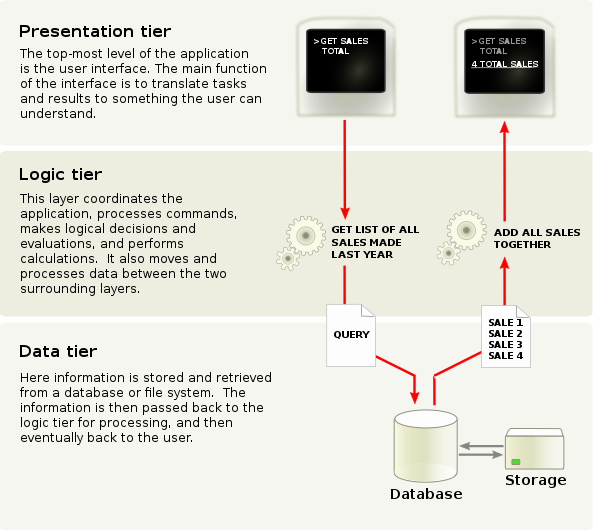
\includegraphics[width=0.66\textwidth]{images/layer.png}
    \caption{Mô hình kiến trúc 3 tầng (3-tiers) \cite{viquynhMVC2}.}
    \label{fig:fig11}
  \end{figure}
    
    
        \hspace*{0.8cm}Cụ thể, lớp Presentation đóng vai trò là điểm tương tác giữa người dùng và hệ thống, chịu trách nhiệm hiển thị thông tin và thu nhận thao tác từ phía người dùng. Lớp Business Logic là nơi xử lý toàn bộ logic nghiệp vụ, từ kiểm tra dữ liệu nhập vào đến các phép tính, xử lý trạng thái và ra quyết định. Cuối cùng, lớp Data đảm nhiệm vai trò giao tiếp với nguồn dữ liệu – có thể là cơ sở dữ liệu cục bộ hoặc server từ xa – và thực hiện các thao tác đọc, ghi hoặc đồng bộ hóa.
    
    
        \vspace{0.5em}
    
        \hspace*{0.8cm}Ưu điểm nổi bật của mô hình Layers là tính phân tách trách nhiệm (separation of concerns). Mỗi lớp chỉ đảm nhiệm một nhóm chức năng chuyên biệt, nên khi có thay đổi hoặc lỗi phát sinh ở một lớp, lập trình viên có thể xử lý mà không ảnh hưởng đến các lớp còn lại. Điều này đặc biệt quan trọng trong các dự án lớn hoặc khi có nhiều lập trình viên cùng tham gia. Ngoài ra, việc kiểm thử (testing) cũng trở nên dễ dàng hơn nhờ tính độc lập giữa các lớp. Tuy nhiên, mô hình này cũng có thể dẫn đến sự phụ thuộc theo chiều dọc giữa các lớp nếu không được thiết kế đúng cách, và đôi khi làm tăng số lượng lớp và khối lượng mã khi ứng dụng phát triển phức tạp hơn.
    
        \vspace{0.5em}
    
        \hspace*{0.8cm}Nhìn chung, kiến trúc phân lớp đóng vai trò như một mô hình nền tảng, thích hợp với nhiều loại ứng dụng khác nhau. Nhờ khả năng tổ chức tốt và dễ mở rộng, mô hình này thường được sử dụng làm cơ sở cho các kiến trúc phức tạp hơn như MVC hay MVVM, đóng góp vào việc xây dựng phần mềm có cấu trúc bền vững và hiệu quả.
    

% 3.2
\subsection{Mẫu kiến trúc MVC}
\renewcommand{\labelitemi}{--}    
    
        \hspace*{0.8cm}Trong số các mô hình kiến trúc phần mềm được áp dụng trên nền tảng iOS, Model View Controller (MVC) là một trong những mô hình lâu đời và phổ biến nhất. MVC chia ứng dụng thành ba thành phần chính, từ đó giúp lập trình viên dễ dàng tổ chức mã nguồn và phân tách nhiệm vụ của từng bộ phận trong quá trình phát triển. Trong đó, thành phần Model đảm nhiệm vai trò quản lý dữ liệu và xử lý các quy tắc nghiệp vụ, đóng vai trò như “bộ não” của ứng dụng. Tiếp theo, thành phần View chịu trách nhiệm hiển thị thông tin tới người dùng, phản ánh đúng trạng thái hiện tại của dữ liệu từ Model. Cuối cùng, thành phần Controller đóng vai trò trung gian, cầu nối giữa View và Model, đảm nhận việc xử lý các sự kiện tương tác của người dùng, đồng thời cập nhật lại giao diện khi dữ liệu thay đổi.
    

    % https://daynhauhoc.com/t/loi-load-du-lieu-len-jsp/109965/10
\begin{figure}[H]
    \centering
    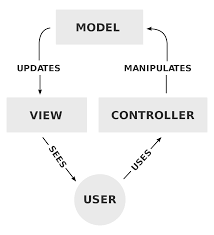
\includegraphics[width=0.44\textwidth]{images/mvc.png}
    \caption{Mô hình kiến trúc MVC \cite{daynhauhocMVC}.}
    \label{fig:fig12}
  \end{figure}

    
      \hspace*{0.8cm}Với cấu trúc như vậy, mô hình MVC mang đến cho lập trình viên iOS một cách tiếp cận đơn giản, dễ hiểu, phù hợp với những người mới bắt đầu tiếp cận lập trình giao diện người dùng. Tuy nhiên, trong thực tế triển khai, một vấn đề lớn phát sinh là hiện tượng “Massive View Controller” \cite{massive_vc}, khi Controller bị quá tải do chứa cả logic giao diện lẫn logic nghiệp vụ. Điều này dẫn đến mã nguồn trở nên khó bảo trì, khó kiểm thử và dễ phát sinh lỗi khi mở rộng chức năng. Chính vì thế, ngày càng nhiều lập trình viên iOS hiện đại chuyển sang các mô hình khác như MVVM hoặc VIPER để giảm thiểu sự phụ thuộc và tách biệt rõ ràng các thành phần chức năng hơn. Nhìn chung, mặc dù MVC vẫn giữ được tính phổ biến nhất định, đặc biệt trong các ứng dụng đơn giản, nhưng nó không còn là lựa chọn tối ưu trong các dự án phức tạp hoặc quy mô lớn.
    

% 3.3
\subsection{Mô hình kiến trúc MVVM}
\renewcommand{\labelitemi}{--}    
    
        \hspace*{0.8cm}Trên nền tảng Android, mô hình kiến trúc Model–View–ViewModel (MVVM) ngày càng trở nên phổ biến nhờ khả năng tương thích cao với các thư viện hỗ trợ hiện đại như LiveData, ViewModel, và Data Binding. MVVM được thiết kế để tách biệt rõ ràng giữa giao diện người dùng và logic nghiệp vụ, đồng thời hỗ trợ tốt cho việc phát triển theo hướng phản ứng (reactive programming). Trong mô hình này, Model tiếp tục đảm nhiệm vai trò quản lý dữ liệu và xử lý các quy tắc nghiệp vụ, tương tự như trong mô hình MVC. View, tức giao diện người dùng, có nhiệm vụ hiển thị dữ liệu và nhận tương tác từ người dùng, tuy nhiên, thay vì xử lý trực tiếp các thao tác đó, View sẽ truyền tín hiệu cho ViewModel để xử lý.
    

    % https://teky.edu.vn/blog/lap-trinh-web-mvc/
\begin{figure}[H]
    \centering
    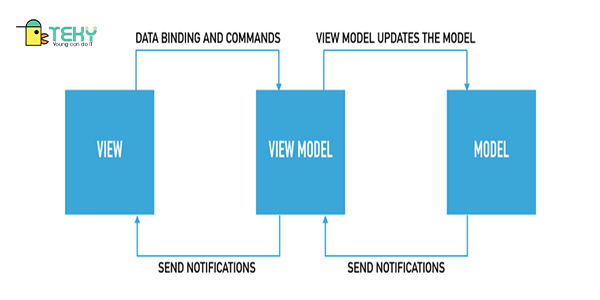
\includegraphics[width=0.67\textwidth]{images/mvvm.jpg}
    \caption{Mô hình kiến trúc MVVM \cite{tekyMVVM}}
    \label{fig:fig13}
  \end{figure}

    
      \hspace*{0.8cm}Thành phần cốt lõi giúp MVVM trở nên nổi bật chính là ViewModel – lớp trung gian giữa View và Model. ViewModel không chứa tham chiếu trực tiếp tới View, mà hoạt động dựa trên cơ chế Observer Pattern, cho phép dữ liệu được quan sát và cập nhật tự động từ ViewModel lên View mỗi khi có thay đổi. Nhờ đó, View trở nên “mỏng” hơn vì chỉ tập trung vào hiển thị, còn toàn bộ logic xử lý sự kiện, tính toán hoặc tương tác với dữ liệu được chuyển giao sang ViewModel. Cách tiếp cận này không những giúp giảm sự ràng buộc giữa các lớp, mà còn tăng khả năng tái sử dụng, kiểm thử tự động và phát triển song song giữa các thành viên trong nhóm \cite{testability_mvvm}.
    
      \vspace{0.5em}
    
        \hspace*{0.8cm}Tóm lại, MVVM phù hợp với xu hướng phát triển ứng dụng hiện đại trên Android khi đặt trọng tâm vào tính phân tách, phản ứng và mở rộng. So với các mô hình truyền thống như MVC, MVVM mang lại kiến trúc rõ ràng hơn và giúp lập trình viên kiểm soát ứng dụng hiệu quả trong cả giai đoạn phát triển lẫn bảo trì.
    

% 3.4
\subsection{Hỗ trợ mô hình Client – Server}
\renewcommand{\labelitemi}{--}    
    
        \hspace*{0.8cm}Trong quá trình xây dựng ứng dụng di động hiện đại, mô hình Client–Server luôn đóng vai trò then chốt trong việc hỗ trợ các chức năng có kết nối mạng. Cả hai nền tảng iOS và Android đều cung cấp đầy đủ công cụ để triển khai mô hình này một cách hiệu quả. Trong mô hình Client–Server, ứng dụng di động đóng vai trò như Client, có nhiệm vụ gửi các yêu cầu (request) tới một máy chủ từ xa (Server) thông qua các giao thức HTTP với các phương thức như GET, POST, PUT, DELET. Sau khi tiếp nhận yêu cầu, Server sẽ xử lý thông tin, truy xuất cơ sở dữ liệu và trả về kết quả dưới dạng JSON hoặc XML để Client hiển thị hoặc xử lý tiếp theo.
    

    % https://codelearn.io/sharing/tim-hieu-ve-mo-hinh-client-server
\begin{figure}[H]
    \centering
    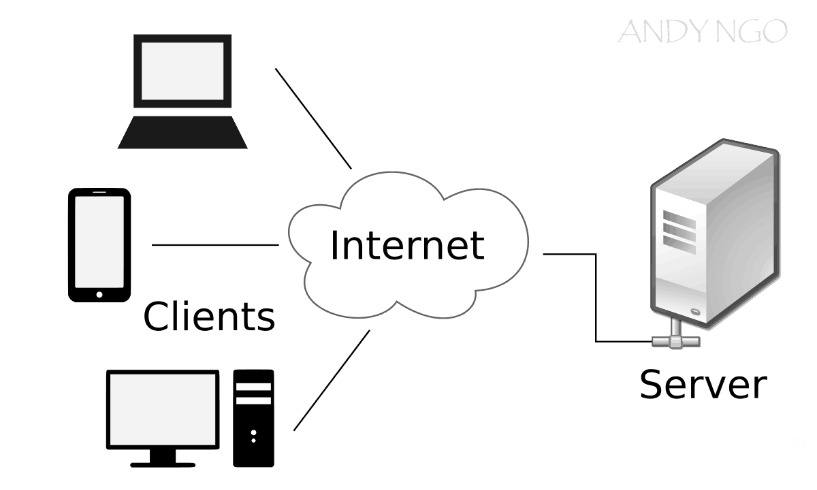
\includegraphics[width=0.75\textwidth]{images/client-server.jpg}
    \caption{Mô hình Client – Server \cite{codelearnClientServer}.}
    \label{fig:fig14}
  \end{figure}

    
      \hspace*{0.8cm}Để hỗ trợ tốt cho mô hình này, các hệ điều hành di động đều cung cấp nhiều thư viện mạnh mẽ. Trên iOS, lập trình viên có thể sử dụng URLSession như một công cụ tiêu chuẩn từ Apple hoặc tích hợp thư viện bên thứ ba như Alamofire để đơn giản hóa các tác vụ mạng. Tương tự, Android cung cấp các thư viện Retrofit và OkHttp giúp việc gửi yêu cầu và xử lý phản hồi trở nên nhanh chóng, dễ mở rộng và dễ kiểm thử. Thông qua mô hình Client–Server, ứng dụng di động có thể hoạt động nhẹ nhàng hơn vì dữ liệu và logic nặng được xử lý ở phía máy chủ. Ngoài ra, tính năng đồng bộ dữ liệu và cập nhật thời gian thực giữa nhiều thiết bị người dùng cũng được hiện thực hóa dễ dàng thông qua mô hình này. Điều này cho thấy Client–Server không chỉ là một mô hình kết nối, mà còn là nền tảng cốt lõi giúp ứng dụng thích ứng linh hoạt trong môi trường đa thiết bị và thay đổi liên tục ngày nay \cite{scalable_mobile_arch}.
    

% 3.5
\subsection{Đánh giá tổng quan}
\renewcommand{\labelitemi}{--}    
    
        \hspace*{0.8cm}Dưới góc nhìn tổng quan, các mô hình kiến trúc phần mềm như MVC, MVVM và Client–Server đều mang đến những giá trị thiết thực trong việc phát triển ứng dụng di động. Tuy nhiên, mỗi nền tảng lại có sự ưu tiên khác nhau trong cách tiếp cận và tổ chức mã nguồn. Đối với nền tảng iOS, mô hình MVC từng được xem là tiêu chuẩn “vàng” nhờ vào sự đơn giản và dễ học. Thế nhưng, hạn chế lớn nhất của MVC – đó là hiện tượng “Massive View Controller” – đã khiến nhiều lập trình viên tìm đến các mô hình thay thế để có được cấu trúc tách biệt và linh hoạt hơn \cite{massive_view_controller}.
    
        \vspace{0.5em}
    
        \hspace*{0.8cm}Trong khi đó, Android hiện đại hóa cách tổ chức ứng dụng thông qua mô hình MVVM, tận dụng sức mạnh từ các thành phần như LiveData, ViewModel và Data Binding. Nhờ vậy, lập trình viên có thể giảm mạnh sự phụ thuộc giữa giao diện và logic nghiệp vụ, đồng thời tối ưu khả năng tái sử dụng và kiểm thử mã nguồn. 

        \vspace{0.5em}
        
        \hspace*{0.8cm}Bên cạnh mô hình kiến trúc, đặc điểm hệ điều hành cũng tác động không nhỏ đến trải nghiệm của lập trình viên trong quá trình phát triển ứng dụng. Trên iOS, sự đồng nhất về phần cứng và phiên bản hệ điều hành giúp giảm thiểu rủi ro phân mảnh, từ đó đơn giản hóa công tác kiểm thử và tối ưu hiệu năng. Tuy nhiên, môi trường phát triển iOS lại yêu cầu lập trình viên phải sử dụng hệ sinh thái phần mềm riêng biệt của Apple như macOS và Xcode, điều này có thể gây bất tiện cho những người không quen thuộc. Ngược lại, Android mở ra không gian phát triển linh hoạt hơn với nhiều lựa chọn công cụ và hệ điều hành, nhưng lại đặt ra thách thức lớn về mặt phân mảnh thiết bị và phiên bản. Lập trình viên Android thường phải kiểm tra ứng dụng trên nhiều cấu hình khác nhau để đảm bảo tính tương thích, đặc biệt là với những ứng dụng cần hiệu năng cao hoặc sử dụng phần cứng chuyên biệt.
        
        \vspace{0.5em}

        \hspace*{0.8cm}Ngoài ra, cả iOS và Android đều đồng thuận trong việc triển khai mô hình Client–Server nhằm tăng khả năng mở rộng, giảm tải cho thiết bị người dùng và hỗ trợ ứng dụng hoạt động ổn định trong môi trường mạng. Việc nắm rõ đặc điểm, ưu điểm cũng như nhược điểm của từng mô hình kiến trúc sẽ giúp lập trình viên không chỉ lựa chọn đúng giải pháp cho từng dự án cụ thể, mà còn góp phần nâng cao hiệu quả phát triển, khả năng bảo trì và mở rộng sản phẩm trong dài hạn.
    

\section{Phân tích chi tiết các kiến trúc phần mềm}

% 
\subsection{Kiến trúc phần mềm ba tầng (Three-tier architecture)}
\renewcommand{\labelitemi}{--}    
    \begin{flushleft}
        \hspace*{0.8cm}Đây là một mô hình tổ chức phần mềm phổ biến, đặc biệt phù hợp với các hệ thống lớn, có khả năng mở rộng và bảo trì lâu dài. Mô hình này phân chia rõ ràng trách nhiệm của từng tầng, từ việc hiển thị, xử lý logic cho đến lưu trữ dữ liệu. Việc áp dụng kiến trúc ba tầng giúp ứng dụng dễ bảo trì, linh hoạt trong mở rộng và tăng khả năng tái sử dụng mã nguồn.
    \end{flushleft}

    \begin{flushleft}
      \hspace*{0.8cm}Kiến trúc ba tầng có thể áp dụng cho nhiều loại ứng dụng khác nhau: từ ứng dụng đơn giản đến phức tạp, từ ứng dụng độc lập đến ứng dụng kết nối mạng. Việc tách biệt ba tầng không chỉ làm cho mã nguồn trở nên rõ ràng hơn mà còn cho phép các nhóm phát triển làm việc độc lập trên từng tầng.
    \end{flushleft}

    \begin{flushleft}
      \hspace*{0.8cm}Tầng trình diễn (Presentation Layer), đây là tầng giao tiếp với người dùng. Chức năng chính của tầng này bao gồm:
      \setlength{\leftmargini}{1.5cm}
      \begin{itemize}
          \item Hiển thị dữ liệu từ tầng nghiệp vụ theo giao diện trực quan.
          \item Nhận lệnh từ người dùng (qua các nút bấm, form, tương tác giao diện).
          \item Không xử lý logic nghiệp vụ, nhờ vậy giao diện có thể dễ dàng tái sử dụng, thay đổi hoặc cập nhật mà không ảnh hưởng đến các tầng khác.
          \item[]$\Rightarrow$ Một lợi ích lớn là khả năng “lắp ghép” lại với các tầng nghiệp vụ khác nhau – giúp cùng một giao diện có thể sử dụng cho nhiều phiên bản khác nhau của hệ thống.
      \end{itemize}
    \end{flushleft}

    \begin{flushleft}
      \hspace*{0.8cm}Tầng nghiệp vụ (Business Logic Layer), tầng này giữ vai trò trung tâm trong hệ thống. Nó thực hiện:
      \setlength{\leftmargini}{1.5cm}
      \begin{itemize}
          \item Chuẩn bị dữ liệu đầu vào để gửi đến tầng dữ liệu.
          \item Chuyển đổi, xử lý dữ liệu nhận về để trả lại cho tầng trình diễn.
          \item Xử lý các lỗi logic hoặc lỗi phản hồi từ tầng dữ liệu.
          \item Áp dụng các quy tắc nghiệp vụ, như kiểm tra hợp lệ, xử lý quy trình.
          \item[]$\Rightarrow$ Tầng này giúp cô lập các xử lý phức tạp khỏi giao diện và dữ liệu, đảm bảo khả năng kiểm thử và bảo trì cao.
      \end{itemize}
    \end{flushleft}

    \begin{flushleft}
      \hspace*{0.8cm}Tầng dữ liệu (Data Layer), là nơi lưu trữ các thông tin quan trọng nhất của ứng dụng:
      \setlength{\leftmargini}{1.5cm}
      \begin{itemize}
          \item Lưu trữ cơ sở dữ liệu (SQL, NoSQL…).
          \item Thực hiện các truy vấn để đảm bảo hiệu năng và độ chính xác cao.
          \item Có thể tích hợp với cơ sở dữ liệu từ xa (server), hệ thống lưu trữ đám mây hoặc tệp cục bộ.
          \item[]$\Rightarrow$ Việc tối ưu tầng dữ liệu giúp cải thiện đáng kể hiệu năng của toàn hệ thống, đặc biệt là trong các ứng dụng có lượng dữ liệu lớn.
      \end{itemize}
    \end{flushleft}

    \begin{flushleft}
      \hspace*{0.8cm}$\Rightarrow$ Kiến trúc ba tầng mang lại lợi ích lớn về mặt tổ chức mã nguồn, bảo trì, kiểm thử và phát triển theo nhóm. Mỗi tầng có trách nhiệm riêng, từ đó giúp ứng dụng dễ mở rộng và thích ứng với thay đổi trong tương lai.
    \end{flushleft}

% 4.2
\subsection{Kiến trúc MVC (Model – View – Controller)}
\renewcommand{\labelitemi}{--}    
    \begin{flushleft}
        \hspace*{0.8cm}MVC (Model – View – Controller) là một mẫu kiến trúc phần mềm cổ điển, phổ biến trong phát triển ứng dụng, đặc biệt là trên nền tảng iOS. Mục tiêu chính của kiến trúc MVC là tách biệt rõ ràng giữa dữ liệu, giao diện và điều khiển xử lý, từ đó giúp ứng dụng dễ bảo trì, mở rộng và nâng cao trải nghiệm người dùng.
    \end{flushleft}

    \begin{flushleft}
      \hspace*{0.8cm}Mô hình này được hình dung như một sơ đồ ba thành phần, mỗi thành phần đảm nhận một vai trò cụ thể:
      \setlength{\leftmargini}{1.5cm}
      \begin{itemize}
          \item Model: Dữ liệu và logic xử lý dữ liệu.
          \item View: Giao diện hiển thị cho người dùng.
          \item Controller: Bộ điều phối, tiếp nhận hành động từ người dùng và điều khiển luồng xử lý.
          \item[]$\Rightarrow$ Ba thành phần hoạt động tách biệt nhưng liên kết chặt chẽ, đảm bảo ứng dụng vận hành trơn tru và dễ dàng điều chỉnh một phần mà không ảnh hưởng đến phần còn lại.
      \end{itemize}
    \end{flushleft}

    \begin{flushleft}
      \hspace*{0.8cm}Model – Mô hình dữ liệu:
      \setlength{\leftmargini}{1.5cm}
      \begin{itemize}
          \item Định danh những gì cần trả về cho người dùng.
          \item Đây là nơi chứa dữ liệu thô, các quy tắc nghiệp vụ và các thao tác xử lý dữ liệu.
          \item Ví dụ: trong một ứng dụng bán hàng, Model chứa thông tin sản phẩm, đơn hàng, người dùng...
      \end{itemize}
    \end{flushleft}

    \begin{flushleft}
      \hspace*{0.8cm}Controller – Bộ điều khiển:
      \setlength{\leftmargini}{1.5cm}
      \begin{itemize}
          \item Tiếp nhận các yêu cầu từ người dùng (qua View).
          \item Thực hiện các truy vấn tài nguyên, gọi các phương thức xử lý trong Model.
          \item Là “bộ não” điều phối mọi hoạt động trong ứng dụng.
      \end{itemize}
    \end{flushleft}

    \begin{flushleft}
      \hspace*{0.8cm}View – Giao diện người dùng:
      \setlength{\leftmargini}{1.5cm}
      \begin{itemize}
          \item Hiển thị dữ liệu dưới dạng dễ hiểu, thân thiện với người dùng.
          \item View không xử lý logic nghiệp vụ, mà chỉ phản hồi lại theo những gì Controller và Model cung cấp.
          \item View sẽ cập nhật nội dung mỗi khi Model thay đổi.
      \end{itemize}
    \end{flushleft}

    \begin{flushleft}
      \hspace*{0.8cm}MVC giúp tách biệt rõ ràng chức năng, dễ dàng phát triển, kiểm thử và bảo trì. Đồng thời cho phép nhiều lập trình viên làm việc song song: người thiết kế giao diện làm View, lập trình viên backend làm Model, còn Controller kết nối hai phần này. Ngoài ra, nó còn có tính tái sử dụng mã nguồn tốt khi một Model có thể được dùng cho nhiều View khác nhau.
    \end{flushleft}

    \begin{flushleft}
      \hspace*{0.8cm}$\Rightarrow$ Mẫu kiến trúc MVC là một giải pháp hiệu quả giúp tổ chức ứng dụng một cách khoa học và linh hoạt. Việc phân chia ứng dụng thành ba thành phần rõ ràng giúp giảm độ phức tạp khi mở rộng, dễ bảo trì, đồng thời nâng cao hiệu quả làm việc nhóm trong quá trình phát triển ứng dụng. Với iOS, MVC vẫn là lựa chọn được ưa chuộng và hỗ trợ tốt trong môi trường phát triển Xcode và Swift.
    \end{flushleft}

% 4.3
\subsection{Kiến trúc MVVM (Model - View - ViewModel)}
\renewcommand{\labelitemi}{--}    
    \begin{flushleft}
        \hspace*{0.8cm}Kiến trúc MVVM (Model – View – ViewModel) là một trong những mẫu thiết kế hiện đại, được áp dụng phổ biến trong phát triển ứng dụng Android (đặc biệt là với sự hỗ trợ từ Jetpack và Kotlin). MVVM ra đời nhằm tối ưu quá trình phát triển ứng dụng bằng cách tách biệt logic hiển thị và logic xử lý, đồng thời tăng tính tự động hóa trong việc cập nhật dữ liệu nhờ cơ chế Data Binding.
    \end{flushleft}

    \begin{flushleft}
      \hspace*{0.8cm}MVVM có cấu trúc gần giống với MVC, nhưng thay vì để Controller điều khiển toàn bộ luồng xử lý, MVVM đưa vào một tầng trung gian là ViewModel – chịu trách nhiệm “kết nối thông minh” giữa dữ liệu (Model) và giao diện (View):
      \setlength{\leftmargini}{1.5cm}
      \begin{itemize}
          \item Tương tự như MVC, View hiển thị dữ liệu, Model chứa dữ liệu và logic xử lý.
          \item Tuy nhiên, Controller được thay thế bằng ViewModel, giúp giảm bớt sự ràng buộc giữa View và Model.
      \end{itemize}
    \end{flushleft}

    \begin{flushleft}
      \hspace*{0.8cm}Model – Dữ liệu và logic xử lý:
      \setlength{\leftmargini}{1.5cm}
      \begin{itemize}
          \item Là nơi lưu trữ các dữ liệu chính của ứng dụng (như thông tin người dùng, sản phẩm...).
          \item Xử lý các nghiệp vụ như tính toán, truy xuất dữ liệu từ cơ sở dữ liệu hoặc API.
          \item Model không trực tiếp liên hệ với View, mà thông qua ViewModel.
      \end{itemize}
    \end{flushleft}

    \begin{flushleft}
      \hspace*{0.8cm}View – Giao diện hiển thị:
      \setlength{\leftmargini}{1.5cm}
      \begin{itemize}
          \item Là phần người dùng tương tác trực tiếp (giao diện ứng dụng).
          \item View trong MVVM không xử lý logic nghiệp vụ mà chỉ phản ánh lại các dữ liệu từ ViewModel.
          \item Nhờ vào Data Binding, View có thể tự động cập nhật khi dữ liệu trong ViewModel thay đổi – giúp giảm mã lặp và tăng hiệu suất phát triển.
      \end{itemize}
    \end{flushleft}

    \begin{flushleft}
      \hspace*{0.8cm}ViewModel – Cầu nối thông minh:
      \setlength{\leftmargini}{1.5cm}
      \begin{itemize}
          \item Chứa các Model và chuẩn bị dữ liệu để hiển thị cho View.
          \item Tạo ra các LiveData hoặc Observable để View có thể theo dõi và tự động cập nhật giao diện khi dữ liệu thay đổi.
          \item Đồng thời, ViewModel cũng xử lý việc truyền dữ liệu từ View sang Model, giúp cập nhật ngược lại khi người dùng nhập liệu hoặc thực hiện thao tác.
      \end{itemize}
    \end{flushleft}

    \begin{flushleft}
      \hspace*{0.8cm}Một điểm mạnh nổi bật của MVVM là cơ chế Data Binding – liên kết dữ liệu hai chiều:
      \setlength{\leftmargini}{1.5cm}
      \begin{itemize}
          \item Khi một đối tượng thuộc nhóm View (như EditText) thay đổi, dữ liệu tương ứng trong ViewModel (hoặc Model) cũng tự động cập nhật.
          \item Ngược lại, khi ViewModel thay đổi giá trị, View cũng cập nhật lại ngay lập tức.
          \item[]$\Rightarrow$ Điều này giúp hạn chế lỗi khi cập nhật giao diện và rút ngắn thời gian phát triển, đặc biệt là trong các ứng dụng có nhiều thao tác tương tác dữ liệu.
      \end{itemize}
    \end{flushleft}

    \begin{flushleft}
      \hspace*{0.8cm}$\Rightarrow$ MVVM là một mô hình kiến trúc mạnh mẽ, phù hợp với các ứng dụng hiện đại cần cập nhật giao diện linh hoạt, liên tục. Với sự hỗ trợ từ Data Binding và LiveData (trong Android), ViewModel giúp đơn giản hóa việc xử lý dữ liệu và đồng bộ giao diện, đồng thời giảm sự phụ thuộc giữa các thành phần, nâng cao khả năng bảo trì và mở rộng về sau. MVVM hiện là lựa chọn ưu tiên trong các dự án Android có quy mô từ vừa đến lớn.
    \end{flushleft}

% 4.4
\subsection{Kiến trúc Client/Server}
\renewcommand{\labelitemi}{--}    
    \begin{flushleft}
        \hspace*{0.8cm}Trong thời đại số, đa số các ứng dụng cần trao đổi dữ liệu qua Internet. Mô hình Client/Server trở thành kiến trúc không thể thiếu, đặc biệt với các ứng dụng có tính năng đồng bộ dữ liệu, chia sẻ thông tin theo thời gian thực, hoặc sử dụng tài nguyên trên máy chủ từ xa. Đồng thời, cần kết hợp với các kiến trúc nội bộ như MVC hoặc MVVM để tối ưu hóa việc xây dựng giao diện và xử lý logic.
    \end{flushleft}

    \begin{flushleft}
      \hspace*{0.8cm}Kiến trúc Client/Server mô tả mô hình trong đó ứng dụng Client (thiết bị người dùng) gửi yêu cầu đến Server (máy chủ từ xa), thường qua HTTP Request, WebSocket, hoặc Web Service. Các chức năng chính bao gồm:
      \setlength{\leftmargini}{1.5cm}
      \begin{itemize}
          \item Client: Gửi yêu cầu (request), hiển thị dữ liệu, tương tác với người dùng.
          \item Server: Xử lý yêu cầu, truy cập cơ sở dữ liệu, trả về dữ liệu kết quả.
          \item[]$\Rightarrow$ Kiến trúc này phù hợp cho các ứng dụng có nhiều người dùng, cần chia sẻ dữ liệu như mạng xã hội, ứng dụng ngân hàng, thương mại điện tử…
      \end{itemize}
    \end{flushleft}
\section{Các yếu tố ảnh hưởng đến chi phí phát triển ứng dụng}

  Chi phí phát triển ứng dụng là một yếu tố quan trọng mà các doanh nghiệp cần cân nhắc kỹ lưỡng trước khi triển khai dự án phần mềm. Trong thực tế, chi phí này không chỉ phụ thuộc vào quy mô hay mục tiêu của sản phẩm, mà còn bị chi phối bởi nhiều yếu tố kỹ thuật và chiến lược khác nhau. Từ đặc điểm của tính năng, kiến trúc hạ tầng, đến vị trí địa lý của đội ngũ phát triển, mỗi yếu tố đều có thể tạo ra sự chênh lệch đáng kể về ngân sách đầu tư. Phần này sẽ trình bày hai nhóm nội dung chính: (1) các yếu tố cốt lõi tác động đến chi phí xây dựng và duy trì ứng dụng, và (2) sự khác biệt về chi phí nhân sự theo khu vực địa lý trên thế giới. Qua đó, doanh nghiệp có thể xác định các điểm cần ưu tiên, tối ưu nguồn lực và lựa chọn chiến lược phát triển phù hợp với điều kiện thực tế của mình.

  
  
% 5.1
\subsection{Các yếu tố chính ảnh hưởng đến chi phí phát triển ứng dụng}
\renewcommand{\labelitemi}{--}  

% https://assets.goodfirms.co/pdfs/how-much-does-it-cost-to-develop-an-app.pdf
  \begin{figure}[H]
    \centering
    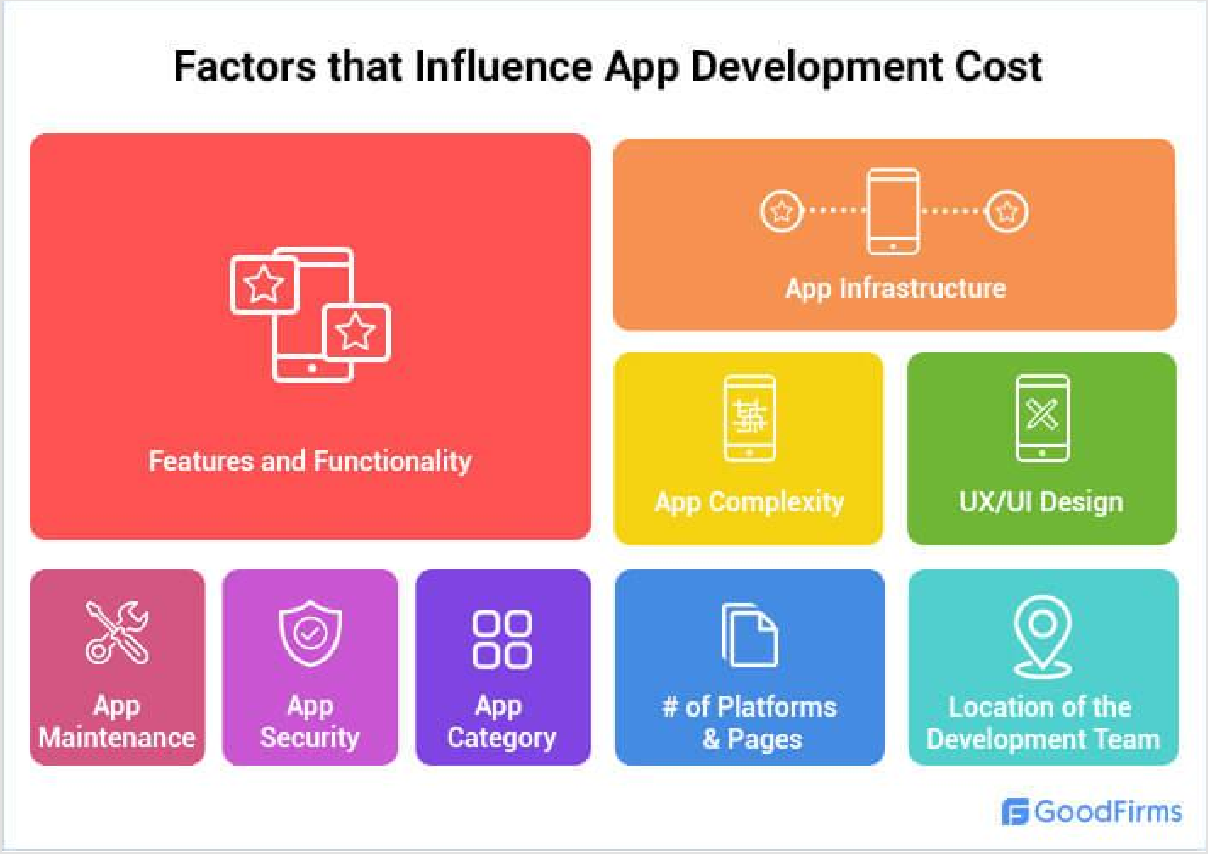
\includegraphics[width=0.6\textwidth]{images/appCosst.png}
    \caption{Các yếu tố chính ảnh hưởng đến chi phí phát triển ứng dụng \cite{goodfirmsAppCost}.}
    \label{fig:fig20}
  \end{figure}

    
      Trong quá trình phát triển ứng dụng, nhiều yếu tố đóng vai trò quyết định đến tổng chi phí, cả trong giai đoạn thiết kế lẫn sau triển khai. Các yếu tố chính bao gồm:
      \setlength{\leftmargini}{1.5cm}
      \begin{itemize}
          \item Tính năng và chức năng (Features and Functionality): Mức độ phức tạp của tính năng tỷ lệ thuận với chi phí phát triển. Ứng dụng có càng nhiều chức năng nâng cao như định vị, livestream, AI tích hợp,… thì đòi hỏi nguồn lực phát triển cao hơn.
          \item Hạ tầng ứng dụng (App Infrastructure): Cách tổ chức hệ thống backend, tích hợp API, hệ thống lưu trữ dữ liệu, bảo mật và tối ưu hiệu năng đều ảnh hưởng lớn đến ngân sách đầu tư. Hạ tầng vững chắc đảm bảo tính ổn định và khả năng mở rộng lâu dài.
          \item Độ phức tạp của ứng dụng (App Complexity): Mức độ phức tạp trong luồng xử lý nghiệp vụ và logic kinh doanh đòi hỏi thời gian phân tích và phát triển dài hơn, từ đó làm tăng chi phí.
          \item Thiết kế trải nghiệm người dùng (UX/UI Design): Giao diện càng trực quan, hiện đại, và thân thiện thì cần đầu tư nhiều thời gian hơn cho thiết kế và kiểm thử.
          \item Chi phí bảo trì (App Maintenance): Sau khi triển khai, ứng dụng cần cập nhật thường xuyên để vá lỗi, cải tiến tính năng hoặc thích nghi với nền tảng mới.
          \item Yêu cầu bảo mật (App Security): Ứng dụng xử lý dữ liệu nhạy cảm (ngân hàng, y tế, tài chính...) đòi hỏi mức độ bảo mật cao, từ đó làm tăng chi phí đầu tư.
          \item Loại ứng dụng (App Category): Tùy thuộc vào lĩnh vực hoạt động (thương mại điện tử, chăm sóc sức khỏe, mạng xã hội…), mức độ phức tạp và chi phí phát triển sẽ khác nhau.
          \item Số lượng nền tảng và màn hình (Number of Platforms \& Pages): Ứng dụng hỗ trợ nhiều nền tảng như iOS, Android, Web với giao diện đa dạng sẽ phát sinh thêm chi phí thiết kế và kiểm thử.
          \item Vị trí nhóm phát triển (Location of the Development Team): Chi phí nhân công thay đổi theo từng khu vực địa lý. Các nhóm tại Mỹ hoặc Tây Âu thường có chi phí cao hơn so với châu Á.
      \end{itemize}
    \vspace{0.5em}

    
      Trong số các yếu tố trên, kiến trúc hạ tầng phần mềm (App Infrastructure) đóng vai trò then chốt:
      \setlength{\leftmargini}{1.5cm}
      \begin{itemize}
          \item Đây là “xương sống” kỹ thuật của toàn bộ hệ thống, quyết định tính ổn định, bảo mật, khả năng tích hợp API, cloud và cơ sở dữ liệu.
          \item Nếu được thiết kế tốt ngay từ đầu, hạ tầng giúp giảm đáng kể chi phí bảo trì và tránh rủi ro gián đoạn trong quá trình vận hành.
      \end{itemize}
    \vspace{0.5em}

% 5.2
\subsection{Chi phí thuê nhân sự theo khu vực địa lý}

\begin{table}[ht]
  \centering
  \begin{tabular}{|l|c|c|c|c|}
  \hline
  \textbf{Title of Employee} & \textbf{United States} & \textbf{Latin America} & \textbf{Eastern Europe} & \textbf{Asia} \\
  \hline
  Business Analyst    & \$110 -- \$205 & \$45 -- \$55 & \$40 -- \$63 & \$30 -- \$42 \\
  Architect           & \$198 -- \$292 & \$60 -- \$72 & \$50 -- \$77 & \$35 -- \$48 \\
  Project Manager     & \$133 -- \$233 & \$55 -- \$66 & \$45 -- \$70 & \$35 -- \$48 \\
  Jr. Developer       & \$105 -- \$111 & \$35 -- \$44 & \$25 -- \$42 & \$18 -- \$24 \\
  Mid-Level Developer & \$132 -- \$140 & \$30 -- \$52 & \$35 -- \$49 & \$25 -- \$34 \\
  Sr. Developer       & \$154 -- \$163 & \$45 -- \$55 & \$45 -- \$70 & \$30 -- \$42 \\
  Lead Developer      & \$176 -- \$187 & \$50 -- \$61 & \$45 -- \$70 & \$35 -- \$50 \\
  Junior QA           & \$77 -- \$81   & \$30 -- \$39 & \$25 -- \$42 & \$20 -- \$30 \\
  Mid-Level QA        & \$99 -- \$105  & \$35 -- \$44 & \$30 -- \$48 & \$25 -- \$32 \\
  Senior QA           & \$143 -- \$169 & \$40 -- \$51 & \$35 -- \$60 & \$30 -- \$40 \\
  Graphic Designer    & \$79 -- \$163  & \$40 -- \$50 & \$35 -- \$56 & \$25 -- \$36 \\
  \hline
  \end{tabular}
  \caption{Mức lương cho các vai trò nhân viên khác nhau trên khắp các khu vực \cite{rubygarageWebCost}.}
  \label{tab:salary-comparison}
  \end{table}
  
\renewcommand{\labelitemi}{--}    
    
        Một trong những yếu tố quan trọng ảnh hưởng đến tổng chi phí phát triển phần mềm chính là chi phí thuê nhân sự theo khu vực địa lý. Các công ty phần mềm, đặc biệt là những doanh nghiệp quốc tế hoặc các dự án có nhu cầu thuê ngoài (outsourcing), thường căn cứ vào mức chi phí trung bình theo giờ làm việc của các vai trò chuyên môn trong ngành công nghệ thông tin để ra quyết định tuyển dụng. Dữ liệu trong bảng ở phần trên được tổng hợp từ 4 khu vực tiêu biểu trên toàn cầu gồm United States (Hoa Kỳ), Latin America (Mỹ Latin), Eastern Europe (Đông Âu) và Asia (Châu Á). Mỗi khu vực có mức chi phí khác nhau rõ rệt, phản ánh sự chênh lệch về mức sống, kỹ năng lao động cũng như nhu cầu thị trường. Thống kê này bao phủ 12 vai trò phổ biến trong các dự án phát triển phần mềm hiện nay, giúp đưa ra cái nhìn tổng quan về chi phí nhân sự theo từng nhóm chức năng.
    \vspace{0.5em}

    
      Đối với nhóm Quản lý và Thiết kế Kiến trúc, mức chi phí thuê nhân sự được ghi nhận là cao nhất trong tất cả các vai trò. Nhóm này bao gồm ba vị trí chủ chốt: Business Analyst (chuyên viên phân tích nghiệp vụ), Architect (kiến trúc sư phần mềm), và Project Manager (quản lý dự án). Trong đó, kiến trúc sư phần mềm đóng vai trò xây dựng khung nền kỹ thuật, đảm bảo hệ thống có thể mở rộng và vận hành ổn định; còn chuyên viên phân tích nghiệp vụ đóng vai trò cầu nối giữa khách hàng và nhóm kỹ thuật; trong khi quản lý dự án là người điều phối toàn bộ tiến độ và tài nguyên. Tại Hoa Kỳ, mức giá thuê cho các vị trí này có thể lên tới gần \$300/giờ – một con số phản ánh tầm quan trọng chiến lược và yêu cầu chuyên môn cao. Mức chi phí này giảm dần tại các khu vực khác, với Latin America và Eastern Europe dao động ở mức trung bình, còn Asia (Châu Á) là nơi có mức chi phí thấp nhất, chỉ từ \$30 – \$48/giờ. Điều này khiến các công ty quốc tế thường ưu tiên thuê ngoài nhóm nhân sự cấp cao từ khu vực châu Á để tiết kiệm chi phí nhưng vẫn đảm bảo hiệu quả.
    \vspace{0.5em}

    
      Tiếp theo là nhóm Lập trình viên (Developer), một trong những thành phần cốt lõi tạo nên sản phẩm phần mềm. Nhóm này được chia nhỏ theo cấp độ kinh nghiệm, bao gồm: Junior Developer, Mid-Level Developer, Senior Developer và Lead Developer. Sự phân loại này phản ánh mức độ độc lập, độ phức tạp của nhiệm vụ mà mỗi cấp độ có thể đảm nhiệm, cũng như ảnh hưởng đến tiến độ và chất lượng sản phẩm. Mức chi phí thuê sẽ tăng tương ứng với cấp độ, từ Junior đến Lead Developer. Tại các khu vực phát triển như Hoa Kỳ, mức lương của Senior hoặc Lead Developer có thể gần tương đương với nhóm kiến trúc sư. Trong khi đó, các khu vực như Latin America hay Eastern Europe có mức chi phí trung bình, phù hợp cho các công ty tầm trung. Asia tiếp tục là khu vực có lợi thế về chi phí, khi mức thuê nhân sự lập trình ở mọi cấp độ đều ở mức thấp hơn đáng kể, giúp các doanh nghiệp tiết kiệm ngân sách mà vẫn có thể tiếp cận với nguồn lực kỹ thuật chất lượng nếu tuyển chọn kỹ lưỡng.
    \vspace{0.5em}

    
      Trong chu trình phát triển phần mềm, kiểm thử phần mềm (QA) là khâu đảm bảo chất lượng đầu ra trước khi triển khai chính thức. Nhóm QA cũng được chia theo cấp độ kinh nghiệm, bao gồm: Junior QA, Mid-Level QA, và Senior QA. So với Developer hoặc Architect, mức chi phí thuê QA thường thấp hơn, nhưng vẫn có sự chênh lệch rõ rệt giữa các khu vực. Tại Mỹ, một Senior QA có thể nhận mức thù lao lên đến \$169/giờ – thậm chí cao hơn Mid-Level Developer tại cùng khu vực (khoảng \$140/giờ). Điều này cho thấy, tại các thị trường phát triển, việc kiểm thử phần mềm được đánh giá rất cao và đòi hỏi kỹ năng chuyên môn sâu. Tại châu Á, các vai trò QA được thuê với mức giá thấp hơn đáng kể, giúp tiết kiệm đáng kể chi phí cho các công ty đang hướng đến tự động hóa kiểm thử hoặc mở rộng nhóm QA.
    \vspace{0.5em}

    
      Cuối cùng là vai trò thiết kế giao diện (Graphic Designer), vốn không yêu cầu chuyên môn kỹ thuật quá sâu như lập trình nhưng vẫn đóng vai trò quan trọng trong việc tạo ra trải nghiệm người dùng hấp dẫn và nhất quán. Tại các thị trường phát triển như Mỹ, chi phí thuê designer vẫn ở mức khá cao do đòi hỏi về thẩm mỹ, khả năng sử dụng công cụ thiết kế chuyên nghiệp và phối hợp chặt chẽ với nhóm phát triển sản phẩm. Trong khi đó, các khu vực như Đông Âu hay châu Á có chi phí thuê thấp hơn đáng kể, đặc biệt phù hợp với các dự án cần thiết kế giao diện ở mức cơ bản đến trung cấp. Việc lựa chọn graphic designer từ các khu vực này giúp doanh nghiệp duy trì ngân sách ở mức hợp lý mà vẫn đảm bảo tính thẩm mỹ và hiệu quả trong giao diện người dùng.
    \vspace{0.5em}

    
      Tóm lại, chi phí thuê nhân sự phát triển phần mềm có sự biến động lớn theo từng khu vực địa lý và vai trò cụ thể. Việc hiểu rõ mức giá trung bình theo giờ và sự khác biệt giữa các nhóm chuyên môn sẽ giúp doanh nghiệp đưa ra chiến lược thuê nhân sự hiệu quả hơn, cân bằng giữa chi phí và chất lượng. Trong bối cảnh toàn cầu hóa và sự phát triển mạnh mẽ của mô hình làm việc từ xa, các công ty hoàn toàn có thể tối ưu hóa nguồn lực bằng cách kết hợp nhân sự ở các khu vực khác nhau, tận dụng lợi thế chi phí của khu vực châu Á và chất lượng kỹ thuật cao từ các khu vực khác để xây dựng đội ngũ phát triển linh hoạt và hiệu quả.





\chapter{Android}
\label{chap:Chap}


\section{Tổng quan về kiến trúc ứng dụng Android}
    % 1.1.
    \subsection{Các ngôn ngữ lập trình sử dụng (Java, các công nghệ đa nền tảng)}
    \renewcommand{\labelitemi}{--}    
    \begin{flushleft}
            \hspace*{0.8cm}Ngôn ngữ lập trình Android là tập hợp các ngôn ngữ được sử dụng để viết ứng dụng cho hệ điều hành Android. Hệ điều hành này phổ biến nhất trên thế giới, với hơn 2 tỷ thiết bị đang hoạt động. Với Android Studio là môi trường phát triển tích hợp chính thức từ Google, việc lập trình ứng dụng Android trở nên dễ dàng hơn bao giờ hết. Ngôn ngữ lập trình Android không chỉ là công cụ để xây dựng các ứng dụng di động phức tạp, mà còn mở ra cơ hội cho các nhà phát triển tạo ra các trải nghiệm đa dạng, từ ứng dụng doanh nghiệp đến trò chơi giải trí độc đáo.
    \end{flushleft}

    \begin{flushleft}
        \hspace*{0.8cm}Các ngôn ngữ lập trình phổ biến nhất cho việc phát triển ứng dụng Android hiện nay:
        \setlength{\leftmargini}{1.5cm}
        \begin{itemize}
            \item Java: Java đã là ngôn ngữ lập trình chính cho Android từ những ngày đầu của nền tảng này. Với cộng đồng lập trình viên lớn và nhiều tài liệu hỗ trợ, Java vẫn là một trong những lựa chọn hàng đầu cho việc phát triển ứng dụng Android.\\
            Ví dụ các ứng dụng đang sử dụng Java : Facebook, WhatApps,…
            \item Kotlin: Kotlin là ngôn ngữ có độ phổ biến ngày càng tăng cho việc phát triển ứng dụng Android. Kotlin cung cấp các tính năng hiện đại và làm cho việc viết mã dễ dàng hơn so với Java. Với sự ủng hộ mạnh mẽ từ Google, Kotlin đang trở thành ngôn ngữ lập trình được ưa chuộng nhất cho Android.\\
            Ví dụ các ứng dụng đang sử dụng Kotlin : Pinterest, Trello,…
            \item Dart: Dart là ngôn ngữ lập trình được sử dụng với framework Flutter – một công nghệ do Google phát triển để xây dựng ứng dụng đa nền tảng (Android, iOS, web, desktop). Dart cho phép lập trình viên viết một lần và triển khai trên nhiều nền tảng, với hiệu suất cao và giao diện người dùng đẹp mắt.\\
            Ví dụ các ứng dụng đang sử dụng Dart (với Flutter): Google Ads, Alibaba, Reflectly,…
        \end{itemize}
    \end{flushleft}

    \begin{flushleft}
        \hspace*{0.8cm}Việc lựa chọn ngôn ngữ lập trình nào để phát triển ứng dụng Android phụ thuộc vào nhiều yếu tố, bao gồm:
        \setlength{\leftmargini}{1.5cm}
        \begin{itemize}
            \item Kinh nghiệm và sở thích của lập trình viên: Nếu bạn đã có kinh nghiệm với Java hoặc Kotlin, bạn có thể sử dụng ngôn ngữ đó để phát triển ứng dụng Android. Nếu bạn mới bắt đầu học lập trình Android, Kotlin có thể là lựa chọn tốt hơn vì nó dễ học hơn Java.
            \item Loại ứng dụng bạn muốn phát triển: Một số ngôn ngữ lập trình phù hợp hơn với các loại ứng dụng nhất định. Ví dụ, C++ là lựa chọn tốt cho các trò chơi, trong khi Python là lựa chọn tốt cho các ứng dụng đơn giản.
            \item Mục tiêu phát triển: Phát triển nhanh(Python, Kotlin), hiệu suất cao(C++), Bảo trì dễ dàng(Java, Kotlin).
            \item Xu hướng thị trường: Kotlin là ngôn ngữ được Google khuyến khích sử dụng cho phát triển ứng dụng Android và đang dần trở nên phổ biến nhờ cú pháp hiện đại và khả năng tương thích tốt. Bên cạnh đó Java vẫn giữ vị trí là ngôn ngữ phổ biến nhất cho Android, tuy nhiên đang dần được thay thế bởi Kotlin trong nhiều dự án mới. Tiếp theo, C++ thường được sử dụng cho các ứng dụng đòi hỏi hiệu suất cao, như game hoặc xử lý đồ họa, nhưng không phổ biến bằng Java hay Kotlin. Trong khi đó, Python ít được sử dụng cho Android do hạn chế về hiệu suất và hỗ trợ nền tảng, tuy nhiên vẫn có thể phù hợp với các ứng dụng đơn giản hoặc phục vụ mục đích học tập, thử nghiệm.        
            \item Hỗ trợ từ cộng đồng: Các ngôn ngữ lập trình phổ biến hơn có cộng đồng hỗ trợ lớn hơn, giúp bạn dễ dàng tìm kiếm trợ giúp khi gặp khó khăn.   
        \end{itemize}
    \end{flushleft}

    % 1.2.
    \subsection{File APK và quá trình đưa ứng dụng lên Google Play, App Store}
    \renewcommand{\labelitemi}{--}
    \begin{flushleft}
        \hspace*{0.8cm}APK (Android Package) là định dạng tập tin được sử dụng để phân phối và cài đặt ứng dụng trên hệ điều hành Android, có đuôi mở rộng .apk, tương tự như .exe trong Windows hoặc .ipa trong IOS. Là gói nén chứa toàn bộ tài nguyên và mã thực thi của ứng dụng.\\
        Cấu trúc bên trong một file APK
        \begin{figure}[H] 
            \centering
            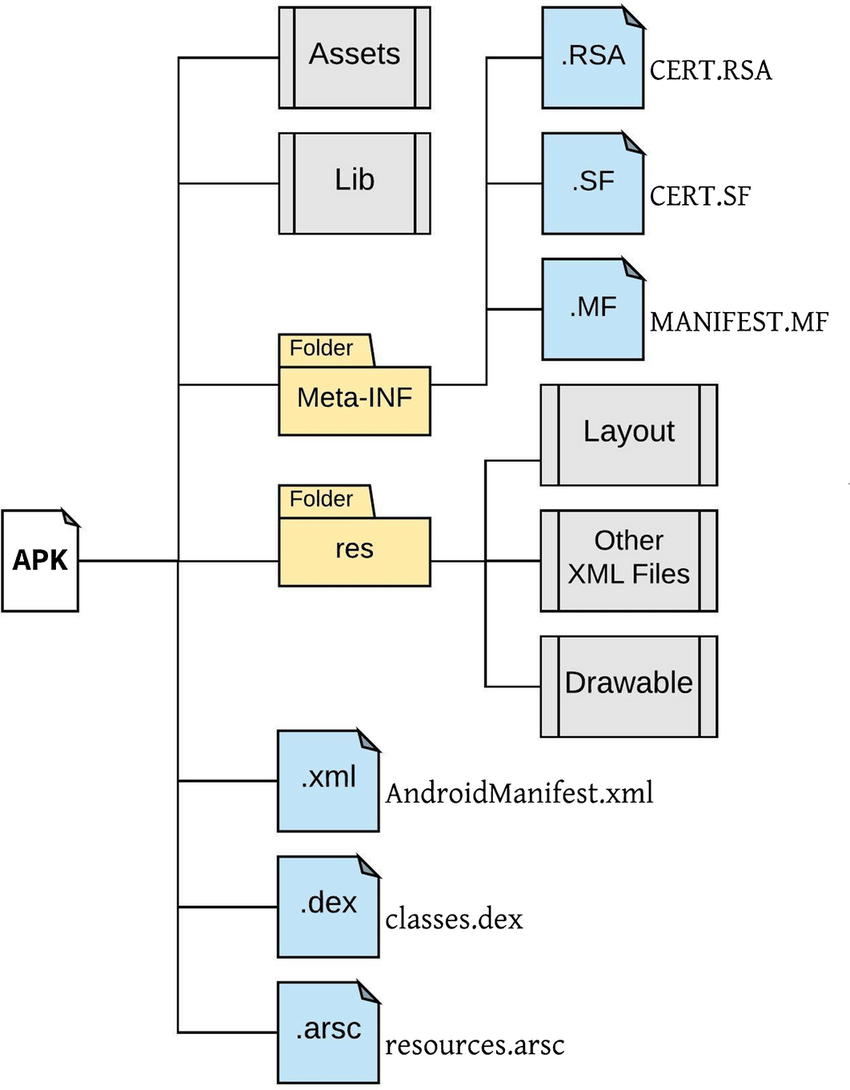
\includegraphics[width=0.5\textwidth]{images/apk.png}
            \caption{Cấu trúc file APK}
            \label{fig:android}
        \end{figure}
        
        \begin{table}[H]
            \centering
            \renewcommand{\arraystretch}{1.5}
            \begin{tabular}{|l|p{11cm}|}
                \hline
                \textbf{Thành phần} & \textbf{Mô tả} \\
                \hline
                \texttt{AndroidManifest.xml} & Chứa thông tin cấu hình ứng dụng: tên gói, phiên bản, các quyền truy cập, khai báo thành phần như Activity, Service, Receiver... \\
                \hline
                \texttt{classes.dex} & Chứa mã bytecode đã được biên dịch từ mã nguồn Java hoặc Kotlin. Đây là phần chính được thực thi trong máy ảo Dalvik hoặc ART. \\
                \hline
                \texttt{resources.arsc} & Tập hợp các tài nguyên đã được biên dịch như chuỗi ký tự (string), style, màu sắc và các giá trị được lưu trong XML. \\
                \hline
                \texttt{res/} & Thư mục chứa các tài nguyên chưa biên dịch như hình ảnh, layout XML, drawable, v.v. \\
                \hline
                \texttt{lib/} & Thư mục chứa các thư viện native (viết bằng C/C++) tương ứng với từng kiến trúc CPU (như ARM, x86...). \\
                \hline
                \texttt{META-INF/} & Lưu trữ các tệp liên quan đến chứng chỉ số, thông tin chữ ký APK để xác thực và bảo vệ toàn vẹn nội dung. \\
                \hline
                \texttt{assets/} & Chứa các tài nguyên thô (raw) do lập trình viên thêm vào, có thể truy cập qua `AssetManager`. \\
                \hline
            \end{tabular}
            \caption{Cấu trúc các thành phần bên trong file APK}
            \label{table:apk-structure}
            \end{table}            
    
        \hspace*{0.8cm}Quy trình khi đưa ứng dụng lên Google Play:  \\
        \setlength{\parskip}{1em}\hspace*{0.6cm}Build APK, từ mã nguồn Android (bằng Android Studio), tạo ra file .apk. Ký số (Signing), ứng dụng được ký bằng private key để xác thực nguồn gốc. Upload lên Google Play, Google kiểm tra, và nếu muốn, có thể dùng App Signing by Google Play, là dịch vụ Google giữ private key. Phân phối và cài đặt, người dùng tải về và cài đặt ứng dụng trực tiếp từ APK.\\

        \hspace*{0.8cm}Tóm lại APK là đơn vị triển khai duy nhất trên Android, có thể chia sẻ trực tiếp (qua web, Bluetooth, email…) mà không cần qua Play Store, dễ dàng trích xuất hoặc phân tích để debug hoặc reverse engineering (nên phải cẩn thận bảo vệ mã nguồn).
    \end{flushleft}

\section{Cơ chế hoạt động của hệ điều hành Android}

% 2.1
\subsection{Android trên nền tảng Linux}
\renewcommand{\labelitemi}{--}    
\begin{flushleft}
    \hspace*{0.8cm}Android được xây dựng trên nhân (kernel) của hệ điều hành Linux, tức là sử dụng Linux kernel làm lớp điều khiển phần cứng như quản lý bộ nhớ, tiến trình, thiết bị ngoại vi và bảo mật hệ thống. Trong khi đó, các thành phần còn lại như giao diện người dùng, framework ứng dụng và dịch vụ hệ thống đều do Google phát triển riêng biệt, không sử dụng giao diện truyền thống của Linux. Android chọn Linux kernel vì đây là nền tảng mã nguồn mở, ổn định, có tính bảo mật cao và hỗ trợ tốt cho các tính năng quan trọng của thiết bị di động như xử lý đa tiến trình, cấp quyền truy cập theo người dùng và hỗ trợ phần cứng đa dạng. Việc kế thừa nhân Linux giúp Android tăng tính linh hoạt, tiết kiệm thời gian phát triển và dễ dàng tùy biến cho từng nhà sản xuất thiết bị.\\
    \newpage
    Google đã tùy biến kernel Linux để phù hợp hơn với điện thoại:
    \begin{table}[H]
        \centering
        \renewcommand{\arraystretch}{1.5}
        \begin{tabular}{|p{3.5cm}|p{12cm}|}
            \hline
            \textbf{Tính năng bổ sung} & \textbf{Công dụng} \\
            \hline
            WakeLocks & Cho phép ứng dụng hoặc hệ thống giữ CPU không rơi vào trạng thái ngủ khi cần thực hiện các tác vụ nền quan trọng, giúp tiết kiệm pin một cách chủ động. \\
            \hline
            Ashmem  & Cung cấp cơ chế chia sẻ vùng nhớ tạm thời giữa các tiến trình, cho phép truyền dữ liệu hiệu quả mà không cần lưu vào bộ nhớ lâu dài. \\
            \hline
            Binder IPC & Là hệ thống giao tiếp liên tiến trình (Inter-Process Communication) do Android phát triển, dùng để truyền dữ liệu và lệnh giữa các app và dịch vụ hệ thống một cách an toàn và nhanh chóng. \\
            \hline
            Logger & Ghi lại thông tin log hệ thống, giúp nhà phát triển theo dõi, phân tích lỗi và hoạt động của ứng dụng hoặc hệ điều hành. \\
            \hline
            Alarm Drivers & Quản lý các sự kiện báo thức (alarm) trong hệ thống, cho phép ứng dụng thực thi tác vụ định kỳ hoặc vào một thời điểm nhất định, kể cả khi thiết bị đang ở trạng thái nghỉ. \\
            \hline
        \end{tabular}
        \caption{Các tính năng bổ sung do Google thêm vào Linux để hỗ trợ hệ điều hành Android}
        \label{table:android-linux-features}
        \end{table}          
\end{flushleft}

\renewcommand{\labelitemi}{--}    
    \begin{flushleft}
        \hspace*{0.8cm}Mỗi ứng dụng gắn với một định danh người dùng riêng. UID (User ID) là mã định danh người dùng cấp hệ điều hành. Trong Android, mỗi ứng dụng (app) được xem như một người dùng độc lập, và hệ thống cấp cho nó một UID riêng biệt.
        \setlength{\leftmargini}{1.5cm}
        \begin{itemize}
            \item Nguồn gốc UID: Android dựa trên Linux kernel, và Linux có mô hình đa người dùng. Mỗi tiến trình (process) trong Linux chạy dưới quyền của một user cụ thể, phân biệt bằng UID.Android tận dụng mô hình này để tăng tính bảo mật cho các ứng dụng.
            \item Mỗi app có vùng dữ liệu riêng (trong /data/data/<tên gói>) mà chỉ UID đó mới truy cập được. Không app nào có thể truy cập trực tiếp vào dữ liệu của app khác, trừ khi quyền được cấp thông qua hệ thống permission và kiểm soát quyền truy cập tập tin, cơ sở dữ liệu, socket. Ghi log và debug app. Cấp phép hoặc từ chối quyền (ví dụ camera, GPS...), do đó UID rất quan trọng.
        \end{itemize}

        \begin{figure}[H] 
            \centering
            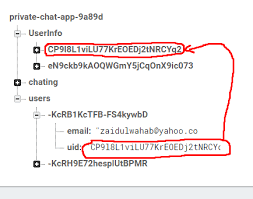
\includegraphics[width=0.5\textwidth]{images/uid.png}
            \caption{Ví dụ về cấu trúc lưu trữ người dùng và thông tin trò chuyện}
            \label{fig:android}
        \end{figure}
    \end{flushleft}

% 2.2
\subsection{Cơ chế sandbox}
\renewcommand{\labelitemi}{--}    
    \begin{flushleft}
        \hspace*{0.8cm}Sandbox trong Android là một môi trường cách ly, nơi mỗi ứng dụng (app) được “nhốt” vào một không gian riêng biệt, không thể trực tiếp can thiệp hay truy cập vào dữ liệu hoặc tiến trình của ứng dụng khác. Hình dung như mỗi app sống trong một “phòng riêng” với cửa khóa, không ai ra vào nếu không có chìa khóa (quyền được cấp).\\
        \setlength{\leftmargini}{1.5cm}
        \hspace*{0.8cm}Cách Android thực hiện sandbox: kết hợp nhiều công nghệ
        \begin{table}[H]
            \centering
            \renewcommand{\arraystretch}{1.5}
            \begin{tabular}{|p{4.5cm}|p{11cm}|}
                \hline
                \textbf{Cơ chế bảo mật} & \textbf{Mục đích} \\
                \hline
                UID riêng biệt cho mỗi app & Mỗi ứng dụng được gán một mã định danh người dùng (UID) riêng biệt, giúp chạy như một "user" độc lập trên nền tảng Linux, cách ly tài nguyên giữa các ứng dụng. \\
                \hline
                Filesystem permissions & Quyền truy cập hệ thống tệp tin được kiểm soát để mỗi ứng dụng chỉ có thể truy cập vào vùng dữ liệu riêng của nó, chẳng hạn như thư mục `/data/data/com.example.app`. \\
                \hline
                Máy ảo (VM) & Mỗi ứng dụng chạy trong một máy ảo riêng (trước đây là Dalvik, hiện tại là ART), giúp cách ly mã thực thi và tăng tính an toàn khi xử lý mã bytecode. \\
                \hline
                Permission system & Nếu ứng dụng muốn truy cập các tài nguyên hệ thống ngoài vùng sandbox như camera, GPS, microphone, hệ thống sẽ yêu cầu xin quyền rõ ràng từ người dùng. \\
                \hline
                SEAndroid & Dựa trên SELinux, SEAndroid bổ sung chính sách bảo mật ở cấp nhân hệ điều hành, kiểm soát hành vi truy cập tài nguyên của từng ứng dụng theo nguyên tắc tối thiểu quyền. \\
                \hline
            \end{tabular}
            \caption{Các cơ chế trong Android đảm bảo môi trường sandbox cho mỗi ứng dụng}
            \label{table:android-sandbox-mechanisms}
            \end{table}
            
    \end{flushleft}

    \begin{flushleft}
      \hspace*{0.8cm}Sandbox bảo vệ những thứ sau:
      \setlength{\leftmargini}{1.5cm}
      \begin{itemize}
          \item Dữ liệu app(database, file, cache...): Không app nào khác có thể truy cập nếu không được cấp quyền
            \item Mã nguồn (classes.dex): Không bị sửa đổi/thay thế bởi app khác
            \item Giao tiếp giữa app: Chỉ có thể qua các cơ chế an toàn như Intent, ContentProvider, Binder
            \item Tài nguyên hệ thống (camera, GPS, v.v.): Chỉ truy cập được nếu người dùng cho phép thông qua hệ thống permission
        \end{itemize}
        \hspace*{0.8cm}Ví dụ: Giả sử có 2 app:
        App1 là ghi chú cá nhân,
        App2 là trò chơi.
        Cơ chế bảo vệ làm cho App2 không thể đọc được ghi chú của App1, trừ khi App1 cung cấp dữ liệu qua Intent, ContentProvider\\
        \hspace*{0.8cm}Tóm lại, Sandbox là lá chắn vô hình bảo vệ mỗi ứng dụng Android như một thế giới riêng biệt. Nó giúp người dùng yên tâm cài đặt nhiều ứng dụng mà không sợ bị can thiệp trái phép
  \end{flushleft}

% 2.3
\subsection{Máy ảo (VM) riêng cho mỗi ứng dụng}

\begin{flushleft}
  \hspace*{0.8cm}Máy ảo là một chương trình mô phỏng một hệ thống máy tính khác, cho phép chạy phần mềm như thể đang chạy trực tiếp trên một máy vật lý. Máy ảo không tương tác trực tiếp với phần cứng, mà thay vào đó hoạt động như một lớp trung gian giữa phần mềm và phần cứng thật. Mỗi máy ảo có môi trường thực thi riêng biệt, được cách ly hoàn toàn, giúp đảm bảo an toàn, ổn định và khả năng quản lý tài nguyên hiệu quả. Trong Android, máy ảo (cụ thể là Dalvik VM hoặc Android Runtime – ART) giữ vai trò trung gian để chạy các ứng dụng Android được biên dịch dưới dạng bytecode. Mã bytecode này được đóng gói trong tệp .dex, và là thành phần quan trọng nằm trong gói cài đặt ứng dụng .apk. Nhờ máy ảo, các ứng dụng có thể được chạy một cách độc lập, không ảnh hưởng đến các ứng dụng khác và bị giới hạn trong vùng tài nguyên mà hệ điều hành cho phép, giúp thực hiện cơ chế sandbox hiệu quả. Máy ảo cũng là yếu tố giúp hệ thống có khả năng phát hiện, cô lập lỗi và ngăn chặn hành vi xâm nhập không mong muốn từ ứng dụng độc hại.
\end{flushleft}

\begin{flushleft}
  \hspace*{0.8cm}Dalvik VM ($Android \leq 4.x$): Là máy ảo đầu tiên của Android,  được thiết kế để chạy các ứng dụng Android trên các thiết bị di động với tài nguyên hạn chế. Dalvik sử dụng register-based architecture, khác với các máy ảo khác như Java Virtual Machine (JVM) vốn dựa trên stack-based architecture. Điều này có nghĩa là phần lớn các phép toán trong Dalvik được thực hiện trên các thanh ghi thay vì bộ nhớ, giúp giảm độ phức tạp và tối ưu hóa hiệu suất. Dalvik còn sử dụng Just-In-Time (JIT) compilation, nghĩa là mã ứng dụng được biên dịch thành mã máy khi ứng dụng đang chạy, thay vì biên dịch toàn bộ trước khi cài đặt. Điều này giúp tiết kiệm bộ nhớ và rút ngắn thời gian cài đặt ứng dụng, vì không cần biên dịch mã trước khi triển khai. Tuy nhiên, Dalvik cũng có một số nhược điểm. Quá trình khởi động ứng dụng có thể bị chậm vì mã phải được biên dịch khi chạy, dẫn đến trải nghiệm người dùng không mượt mà. Bên cạnh đó, hiệu suất tổng thể của Dalvik cũng không cao bằng các máy ảo khác, vì việc biên dịch mã trong thời gian chạy có thể gây ra sự chậm trễ trong quá trình thực thi ứng dụng. Mặc dù vậy, Dalvik vẫn là nền tảng quan trọng trong sự phát triển của Android cho đến khi được thay thế bởi ART (Android Runtime) trong các phiên bản Android sau này.
  Dùng từ Android 1.0 đến Android 4.4 (KitKat).
  \begin{figure}[H] 
    \centering
    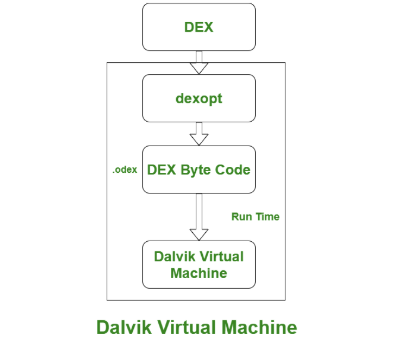
\includegraphics[width=0.6\textwidth]{images/DalvikVM.png}
    \caption{Máy ảo Dalvik}
    \label{fig:android}
\end{figure}  
\end{flushleft}

\begin{flushleft}
    \hspace*{0.8cm}ART (Android Runtime): Thay thế Dalvik từ Android 5.0 (Lollipop), dùng AOT (Ahead-Of-Time) compilation để mã được biên dịch thành mã máy ngay khi cài app.
    Lợi ích là khởi chạy nhanh, hiệu suất cao.
    Nhược điểm là cài đặt lâu hơn, chiếm nhiều bộ nhớ.
    Sau Android 7.0, ART còn hỗ trợ thêm JIT lẫn AOT do đó tối ưu thời gian chạy lẫn bộ nhớ.   
    \begin{figure}[H] 
        \centering
        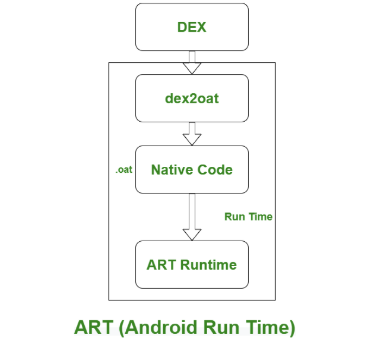
\includegraphics[width=0.6\textwidth]{images/ART.png}
        \caption{Android Run Time}
        \label{fig:android}
    \end{figure}  
\end{flushleft}

\begin{flushleft}
    \hspace*{0.8cm}Quy trình thực thi của Dalvik VM và ART:
    \begin{table}[H]
        \centering
        \renewcommand{\arraystretch}{1.5}
        \begin{tabular}{|p{4cm}|p{5cm}|p{5cm}|}
        \hline
        \textbf{Giai đoạn} & \textbf{Dalvik VM} & \textbf{ART (Android Runtime)} \\
        \hline
        Khi cài đặt ứng dụng & Chép file \texttt{.dex} vào hệ thống & Biên dịch \texttt{.dex} thành mã máy \texttt{.oat} \\
        \hline
        Khi chạy ứng dụng & Dịch bytecode thành mã máy trong thời gian thực (JIT) & Chạy mã máy đã được biên dịch sẵn (AOT) \\
        \hline
        Khi mở lại ứng dụng & Vẫn phải dịch lại bytecode & Khởi động rất nhanh, không cần biên dịch lại \\
        \hline
        \end{tabular}
        \caption{So sánh quá trình thực thi ứng dụng giữa Dalvik VM và ART}
        \label{tab:dalvik-vs-art}
        \end{table}
          
    \hspace*{0.8cm} Lý do Google chuyển từ Dalvik sang ART: Hiệu suất tăng mạnh (app khởi động nhanh hơn), tiết kiệm pin hơn, tối ưu RAM và bộ nhớ tốt hơn, chuẩn bị cho tương lai với các công nghệ như: Android Instant Apps, Dynamic Delivery
\end{flushleft}

\renewcommand{\labelitemi}{--}    
    \begin{flushleft}
        \hspace*{0.8cm}Mỗi ứng dụng là một tiến trình độc lập. Trong Android, mỗi ứng dụng (app) khi được khởi chạy sẽ được cấp phát một tiến trình riêng biệt (process). Tiến trình này có vùng nhớ riêng, UID riêng, máy ảo riêng, hoạt động độc lập, không can thiệp lẫn nhau.
    \end{flushleft}
\newpage
    \begin{flushleft}
      \setlength{\leftmargini}{1.5cm}
      \begin{itemize}
        \item Lợi ích: App không thể truy cập dữ liệu, bộ nhớ hay tiến trình của app khác (bảo mật), nếu 1 app lag/crash, không ảnh hưởng app khác(tối ưu hiệu năng), có thể theo dõi, dừng, hoặc khởi động lại tiến trình một cách riêng lẻ(quản lí tài nguyên), khi hệ thống cần RAM, Android có thể tắt tiến trình app ít dùng mà không ảnh hưởng toàn hệ thống(tự động giải phóng)
        \item Android tạo ra một tiến trình mới: khi người dùng mở ứng dụng lần đầu, app được khởi động lại sau khi bị hệ thống giải phóng
        \item Vùng nhớ riêng trong mỗi tiến trình: mỗi tiến trình chỉ "thấy" được biến, đối tượng trong phạm vi của nó, dữ liệu trong thư mục app, không thể trực tiếp truy cập đến vùng nhớ của tiến trình khác (do cơ chế sandbox, UID, VM kết hợp bảo vệ).
      \end{itemize}
    \end{flushleft}

\section{Chia sẻ dữ liệu giữa các ứng dụng}

\begin{flushleft}
  \hspace*{0.8cm}Trong hệ điều hành Android, mỗi ứng dụng khi được cài đặt sẽ hoạt động như một thực thể độc lập, được bảo vệ bằng cơ chế sandbox. Cơ chế này ngăn cản ứng dụng truy cập trực tiếp vào dữ liệu của ứng dụng khác, giúp nâng cao tính bảo mật và quyền riêng tư cho người dùng. Tuy nhiên, trong một số tình huống thực tế, các ứng dụng vẫn cần khả năng chia sẻ dữ liệu cho nhau. Ví dụ, một ứng dụng chỉnh sửa ảnh có thể cần truy cập đến bộ sưu tập ảnh, hoặc một ứng dụng mạng xã hội cần truy cập danh bạ để đề xuất kết bạn. Để hỗ trợ nhu cầu này mà vẫn đảm bảo an toàn, Android cung cấp một số cơ chế chuẩn để chia sẻ dữ liệu giữa các ứng dụng một cách kiểm soát và có chọn lọc.
\end{flushleft}

% 3.1
\subsection{Cơ chế dùng chung User-id}
\renewcommand{\labelitemi}{--}    
    \begin{flushleft}
        \hspace*{0.8cm}Đây là một điểm trong bảo mật và cấp quyền của Android Các ứng dụng Android có thể dùng chung user-id nếu có cùng chứng chỉ số (digital certificate)
        \setlength{\leftmargini}{1.5cm}
        \begin{itemize}
            \item Mặc định khi một ứng dụng được cài đặt, hệ điều hành Android sẽ tạo một UID (User ID) riêng biệt cho nó, mỗi app chỉ có thể truy cập tài nguyên của chính nó (sandbox).
            \item Hai hoặc nhiều ứng dụng có thể dùng chung UID nếu chúng được ký bằng cùng một khóa chứng thực số (digital certificate) và chúng khai báo "android:sharedUserId" giống nhau trong AndroidManifest.xml
            \item Yêu cầu bắt buộc là chứng chỉ số giống nhau, Android dùng digital signature để đảm bảo chỉ các app thuộc cùng một nhà phát triển mới có thể chia sẻ UID. Điều này ngăn chặn app lạ cố tình khai báo sharedUserId để xâm nhập dữ liệu của app khác.
            Ví dụ nếu app A và app B có sharedUserId giống nhau nhưng ký bằng chứng chỉ khác nhau → Hệ thống từ chối cài đặt!
            \item Lợi ích là các app có thể truy cập dữ liệu và file của nhau, có thể dùng chung database, file cấu hình…, có thể chia sẻ quyền như đọc SMS, camera… nếu quyền được cấp
        \end{itemize}
    \end{flushleft}

% 3.2
\subsection{ContentProvider và Intent}    
    \begin{flushleft}
        \hspace*{0.8cm}Một trong những cơ chế chia sẻ dữ liệu quan trọng nhất trong Android là ContentProvider. Đây là một lớp trung gian cho phép một ứng dụng cung cấp quyền truy cập có kiểm soát đến dữ liệu của mình cho các ứng dụng khác. ContentProvider hoạt động giống như một cơ sở dữ liệu với API chuẩn, cho phép các ứng dụng khác thực hiện thao tác như đọc, ghi, sửa hoặc xóa thông tin, nhưng chỉ trong phạm vi mà nhà phát triển cho phép. Ví dụ điển hình là ứng dụng Danh bạ của Android – nó triển khai một ContentProvider cho phép các ứng dụng khác như Zalo, Facebook hay Viber truy xuất thông tin liên lạc, nhưng chỉ sau khi người dùng đồng ý cấp quyền.\\
        \hspace*{0.8cm}Ngoài ContentProvider, Android còn hỗ trợ chia sẻ dữ liệu thông qua các Intent. Intent là một cơ chế giao tiếp giữa các thành phần trong Android, có thể được sử dụng để truyền dữ liệu giữa các Activity, Service, hoặc giữa các ứng dụng khác nhau. Khi một ứng dụng muốn gửi một tập tin, một đoạn văn bản, hình ảnh hoặc bất kỳ dữ liệu nào sang ứng dụng khác (ví dụ như chia sẻ ảnh lên mạng xã hội), nó có thể tạo một Intent có chứa dữ liệu và gọi startActivity hoặc startActivityForResult. Ứng dụng nhận dữ liệu sẽ phải khai báo rõ ràng trong AndroidManifest.xml các intent filter phù hợp để có thể tiếp nhận loại dữ liệu đó. Cơ chế này đơn giản, phổ biến, và rất hiệu quả cho các thao tác chia sẻ ngắn hạn, không yêu cầu truy cập thường xuyên.\\
        \hspace*{0.8cm}Một phương pháp khác nữa là sử dụng bộ nhớ ngoài (external storage), tức là các file được lưu trên thẻ nhớ hoặc phân vùng có thể truy cập công khai. Trước đây, bất kỳ ứng dụng nào có quyền đọc/ghi vào bộ nhớ ngoài đều có thể truy cập dữ liệu của ứng dụng khác lưu ở đó. Tuy nhiên, kể từ Android 10 (API 29), Google đã giới thiệu cơ chế Scoped Storage để hạn chế quyền truy cập tự do này. Scoped Storage yêu cầu ứng dụng chỉ có thể truy cập vào thư mục riêng của mình trên bộ nhớ ngoài hoặc các file cụ thể được chia sẻ thông qua MediaStore hoặc Storage Access Framework. Điều này đảm bảo rằng không có ứng dụng nào có thể âm thầm đọc hoặc ghi lên dữ liệu của ứng dụng khác mà không có sự cho phép rõ ràng.
    \end{flushleft}

% 3.3
\subsection{FileProvider}
\renewcommand{\labelitemi}{--}    
    \begin{flushleft}
        \hspace*{0.8cm}Một cách hiện đại và an toàn để chia sẻ dữ liệu giữa ứng dụng là sử dụng các API do hệ thống quản lý như FileProvider. Đây là một lớp đặc biệt giúp ứng dụng có thể chia sẻ tệp tin thông qua URI mà không cần cấp quyền truy cập bộ nhớ ngoài toàn cục. FileProvider chỉ cấp quyền truy cập tạm thời, đúng với tệp mà ứng dụng chia sẻ, và chỉ dành cho ứng dụng nhận cụ thể trong một khoảng thời gian nhất định. Điều này giúp tránh được việc ứng dụng khác có thể lén đọc toàn bộ dữ liệu người dùng mà không được cho phép.
    \end{flushleft}
    \begin{flushleft}
      \hspace*{0.8cm}$\Rightarrow$ Tóm lại, Android cung cấp nhiều phương thức để chia sẻ dữ liệu giữa các ứng dụng, mỗi phương thức phù hợp với từng nhu cầu khác nhau. Tuy nhiên, tất cả các cơ chế này đều được thiết kế với tiêu chí an toàn và bảo vệ quyền riêng tư người dùng. Việc chia sẻ dữ liệu phải luôn được thực hiện thông qua cơ chế kiểm soát, có sự đồng ý của người dùng, và hạn chế tối đa quyền truy cập không cần thiết. Trong thời điểm hiện tại, Google cũng khuyến khích các nhà phát triển di chuyển sang những cơ chế chia sẻ an toàn như FileProvider, ContentProvider hoặc sử dụng các API hệ thống để tương tác dữ liệu.
    \end{flushleft}

% 3.4
\subsection{Một số quyền truy cập phổ biến}
    \begin{flushleft}
        \hspace*{0.8cm}Trong quá trình phát triển ứng dụng Android, nhà phát triển thường cần truy cập đến các tài nguyên nhạy cảm trên thiết bị, và mỗi loại tài nguyên đều tương ứng với một hoặc nhiều quyền truy cập cụ thể mà ứng dụng cần khai báo trong file AndroidManifest.xml, đồng thời phải xin phép người dùng tại thời điểm chạy (runtime) nếu thuộc nhóm nguy hiểm. Ví dụ, để truy cập danh bạ người dùng, ứng dụng cần khai báo quyền android.permission.READ-CONTACTS. Đây là quyền nguy hiểm vì liên quan đến thông tin cá nhân, nên bắt buộc phải xin người dùng cho phép khi chạy ứng dụng.\\
        \hspace*{0.8cm}Tương tự, nếu ứng dụng cần gửi hoặc nhận tin nhắn SMS, nhà phát triển phải sử dụng các quyền như SEND-SMS, RECEIVE-SMS và READ-SMS. Đây là những quyền cực kỳ nhạy cảm, liên quan đến quyền riêng tư và chi phí tài chính của người dùng, nên Android yêu cầu phải có lý do rõ ràng và được người dùng cho phép rõ ràng tại runtime.\\
        \hspace*{0.8cm}Việc truy cập thông tin trạng thái thiết bị, như số IMEI hay tình trạng cuộc gọi, đòi hỏi quyền READ-PHONE-STATE. Tuy nhiên, kể từ Android 10, quyền này bị giới hạn mạnh và chỉ cho phép truy cập một số thông tin cơ bản, trừ khi ứng dụng được cấp quyền đặc biệt thông qua Google Play Console. Đối với thông tin vị trí, Android cung cấp hai loại quyền là ACCESS-FINE-LOCATION (vị trí chính xác qua GPS) và ACCESS-COARSE-LOCATION (vị trí tương đối qua mạng). Từ Android 10 trở đi, hệ thống yêu cầu người dùng phải xác định rõ ứng dụng có được quyền truy cập vị trí liên tục không, hay chỉ khi đang sử dụng.\\
        \hspace*{0.8cm}Truy cập vào phần cứng như camera và micro cũng cần xin quyền rõ ràng. Để sử dụng camera, ứng dụng cần có android.permission.CAMERA, và để ghi âm giọng nói, phải khai báo android.permission.RECORD-AUDIO. Cả hai quyền này đều được xếp vào nhóm quyền nhạy cảm, yêu cầu phải xin ở runtime và được người dùng cấp phép rõ ràng. Ngoài ra, để tăng tính minh bạch và tuân thủ chính sách Google Play, ứng dụng cũng nên thông báo trước cho người dùng về lý do cần các quyền này và cách chúng sẽ được sử dụng.
    \end{flushleft} 
\newpage

\section{Ưu điểm của việc sử dụng ngôn ngữ Java trong lập trình Android}
        Java là một trong những ngôn ngữ lập trình lâu đời và phổ biến nhất trên thế giới. Việc sử dụng Java trong lập trình Android giúp lập trình viên dễ dàng tiếp cận với nguồn tài nguyên phong phú từ tài liệu học tập, ví dụ thực tế đến sự hỗ trợ từ cộng đồng. Java sử dụng hệ thống kiểu dữ liệu chặt chẽ(strongly typed), giúp phát hiện lỗi cú pháp và logic ngay trong quá trình biên dịch. Điều này làm tăng độ an toàn của chương trình và giảm thiểu nguy cơ phát sinh lỗi trong quá trình thực thi.

        \vspace{0.5em}

        Một trong những triết lý cốt lõi của Java là “Write once, run anywhere” – nghĩa là mã nguồn chỉ cần viết một lần và có thể chạy trên nhiều nền tảng khác nhau mà không cần chỉnh sửa. Điều này có được là nhờ Java chạy trên máy ảo JVM, giúp mã được biên dịch thành bytecode độc lập với hệ điều hành. Khi lập trình Android bằng Java, điều này đồng nghĩa với việc bạn có thể dễ dàng tái sử dụng phần lớn mã nguồn cho các ứng dụng chạy trên nền tảng khác như desktop hoặc server-side Java.

        \vspace{0.5em}

        Hệ sinh thái phát triển rất phong phú với hàng loạt công cụ và thư viện hỗ trợ mạnh mẽ, tiêu biểu như Android Studio – môi trường phát triển chính thức cho Android. Ngoài ra, Gradle giúp tự động hóa quá trình build, còn hàng nghìn thư viện mã nguồn mở khác có thể giúp giảm đáng kể thời gian và công sức viết mã. Hơn nữa, cộng đồng lập trình viên Java rất đông đảo và hoạt động tích cực, giúp bạn dễ dàng tìm được câu trả lời cho các vấn đề kỹ thuật trên các diễn đàn như Stack Overflow, GitHub, hay cộng đồng Google Developer.

        \vspace{0.5em}

        Java hỗ trợ cơ chế quản lý bộ nhớ tự động thông qua trình thu gom rác(Garbage Collector). Thay vì phải tự giải phóng bộ nhớ như trong C hoặc C++, lập trình viên Java không cần lo lắng về việc quản lý tài nguyên thủ công. Trình thu gom rác sẽ tự động theo dõi và thu hồi vùng nhớ không còn được sử dụng, giúp ngăn ngừa các lỗi phổ biến như rò rỉ bộ nhớ(memory leak) và tăng độ ổn định của ứng dụng, nhất là trong môi trường như Android – nơi tài nguyên hệ thống bị giới hạn \cite{java-tutorial}.
    
        \begin{figure}[H]
            \centering
            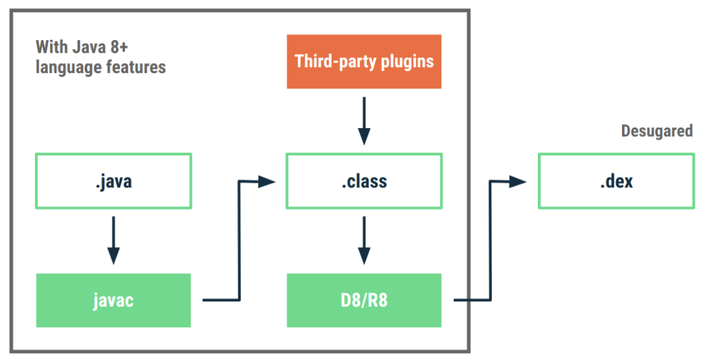
\includegraphics[width=0.8\textwidth]{images/javainandroid.png}
            \caption{Hỗ trợ tính năng ngôn ngữ Java 8 bằng cách desugar biến đổi mã byte \cite{java8}.}
            \label{fig:android2}
        \end{figure}
        
        Trình bổ trợ Android cho Gradle cung cấp khả năng hỗ trợ tích hợp để sử dụng một số tính năng ngôn ngữ Java 8 cùng các thư viện bên thứ ba sử dụng những tính năng đó. Chuỗi công cụ mặc định triển khai các tính năng ngôn ngữ mới bằng cách thực hiện các biến đổi mã byte(được gọi là desugar) như một phần của quá trình biên dịch các tệp lớp D8/R8 thành mã DEX, như minh hoạ trong hình \cite{java8}.


\chapter{IOS}
\label{chap:IOS}


\section{Nền tảng iOS và các thành phần cơ bản}
\hspace*{0.8cm}iOS là hệ điều hành di động do Apple phát triển, được sử dụng chủ yếu trên các thiết bị như iPhone, iPad và iPod Touch. Với kiến trúc nhiều tầng cùng hệ sinh thái phong phú, iOS cung cấp môi trường ổn định, bảo mật và hiệu năng cao cho việc phát triển ứng dụng di động. Để xây dựng một ứng dụng iOS hiệu quả, lập trình viên cần nắm vững các thành phần cơ bản như vòng đời ứng dụng, delegate, giao diện người dùng, cũng như các mô hình kiến trúc phổ biến. Phần này sẽ trình bày tổng quan về các yếu tố cốt lõi tạo nên nền tảng iOS và vai trò của chúng trong quy trình phát triển ứng dụng.
    \subsection{Kiến trúc tầng của iOS}
        \begin{flushleft}
            \begin{figure}[H] % hoặc [h], [t], [b] tùy vị trí
                \centering
                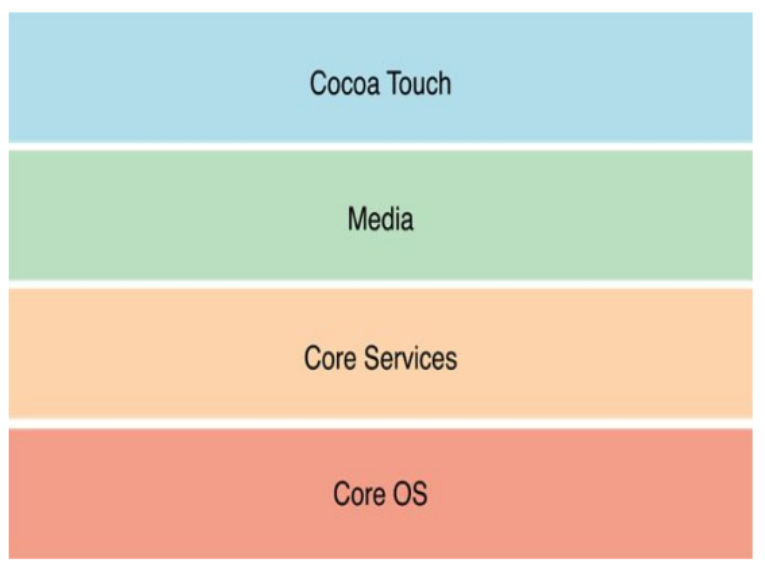
\includegraphics[width=0.8\textwidth]{images/kientrucios.png}
                \caption{Kiến trúc phân tầng IOS\cite{kientrucios}.}
                \label{fig:kientrucios}
            \end{figure}

            \hspace*{0.8cm}Hệ điều hành iOS được tổ chức theo kiến trúc nhiều tầng, trong đó mỗi tầng đảm nhận một vai trò cụ thể và cung cấp các framework cũng như dịch vụ khác nhau. Ở tầng cao nhất, \textbf{Cocoa Touch} cung cấp các framework cốt lõi dành cho việc xây dựng giao diện người dùng, đáng chú ý là \textit{UIKit} và \textit{SwiftUI}. Các công nghệ đồ họa, âm thanh và video như \textit{Core Graphics}, \textit{Core Animation}, và \textit{AVFoundation} được tập trung tại tầng \textbf{Media}, giúp xử lý các chức năng đa phương tiện. Bên dưới đó, tầng \textbf{Core Services} cung cấp các dịch vụ nền tảng cần thiết như \textit{Core Data} để quản lý dữ liệu, \textit{Core Location} để định vị, và \textit{Foundation framework} cho các chức năng cơ bản. Cuối cùng, tầng \textbf{Core OS} đóng vai trò là nền tảng thấp nhất của hệ điều hành, nơi tích hợp kernel, hệ thống tệp, các cơ chế bảo mật và các dịch vụ hệ thống cấp thấp.

       
        \end{flushleft}
   \subsection{ Vòng đời ứng dụng IOS}	
        \begin{flushleft}
            \hspace*{0.8cm}Khi người dùng khởi động điện thoại, chỉ có các thành phần của hệ điều hành (\textit{Operating System}) được phép hoạt động, trong khi các ứng dụng của người dùng chưa được kích hoạt. Các ứng dụng, bao gồm cả ứng dụng của bạn, sẽ chỉ bắt đầu thực thi khi người dùng nhấn vào biểu tượng ứng dụng trên màn hình chính. Chính lúc đó, \textbf{Springboard} – trình quản lý giao diện màn hình chính của iOS – sẽ chịu trách nhiệm kích hoạt ứng dụng. Ứng dụng cùng với các thư viện liên quan sẽ được tải vào bộ nhớ và bắt đầu khởi chạy, trong khi đó \textbf{Springboard} sẽ hiển thị màn hình khởi động (launch screen) để tạo cảm giác phản hồi tức thì cho người dùng. Sau khi quá trình tải hoàn tất, ứng dụng sẽ bắt đầu thực thi, và \texttt{AppDelegate} – đối tượng chịu trách nhiệm quản lý vòng đời của ứng dụng 
            – sẽ nhận được các thông báo tương ứng từ hệ thống.
            Trong quá trình hoạt động, ứng dụng iOS luôn ở một trong các trạng thái xác định: \textbf{Not Running}, \textbf{Inactive}, \textbf{Active}, \textbf{Background}, hoặc \textbf{Suspended}. Những trạng thái này phản ánh tình huống hiện tại của ứng dụng đối với hệ điều hành, và tại bất kỳ thời điểm nào, ứng dụng của bạn đều sẽ nằm trong một trong các trạng thái đó. Việc hiểu rõ và xử lý đúng các trạng thái này là yếu tố then chốt để đảm bảo ứng dụng vận hành hiệu quả, tiết kiệm tài nguyên và mang lại trải nghiệm người dùng mượt mà.
            
        \end{flushleft}
        \begin{figure}[H] % hoặc [h], [t], [b] tùy vị trí
            \centering
            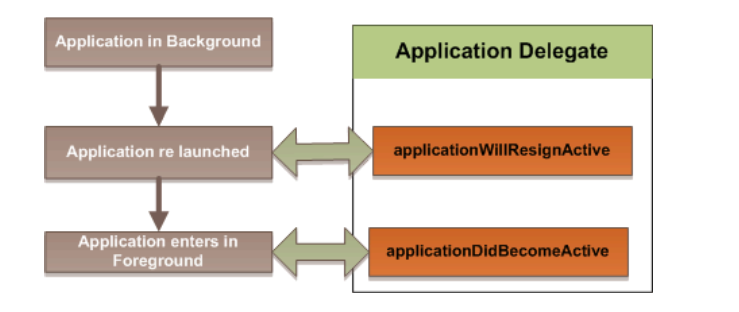
\includegraphics[width=0.8\textwidth]{images/vongdoiios.png}
             \caption{Vòng đời ứng dụng IOS\cite{life cycle-IOS}.} 
            \label{fig:vongdoiios}
        \end{figure}
         \begin{flushleft}
            \textbf{NotRunning:}Ứng dụng chưa được khởi chạy hoặc đã bị hệ thống chấm dứt.
            \textbf{Inactive:} Ứng dụng đang chạy ở foreground nhưng không nhận events (ví dụ: khi có cuộc gọi đến).\\
            \textbf{Active:} Trạng thái bình thường khi ứng dụng chạy ở foreground và đang xử lý events.\\
            \textbf{Background:} Ứng dụng không hiển thị nhưng vẫn chạy và thực thi mã.\\
            \textbf{Suspended:} Ứng dụng ở background nhưng không chạy mã, có thể bị hệ thống chấm dứt để giải phóng tài nguyên.
         \end{flushleft}
         \subsection{App Delegate và Scene Delegate}
         \hspace*{0.8cm}Trong iOS, hai thành phần quan trọng đảm nhận việc quản lý vòng đời và giao diện của ứng dụng là \textbf{AppDelegate} và \textbf{SceneDelegate}. \textbf{AppDelegate}\cite{ App-Scene Delegate} chịu trách nhiệm xử lý các sự kiện cấp cao liên quan đến vòng đời tổng thể của ứng dụng, chẳng hạn như khi ứng dụng được khởi động, chuyển sang chế độ nền, hoặc bị chấm dứt. Bên cạnh đó, nó cũng đảm nhiệm các tác vụ cấu hình ban đầu như đăng ký notification, khởi tạo dịch vụ, và thiết lập dữ liệu dùng chung.
         Kể từ iOS 13, Apple giới thiệu khái niệm \textbf{Scene} để hỗ trợ việc chạy nhiều cửa sổ giao diện (\textit{multi-window}) trong cùng một ứng dụng, đặc biệt trên iPad. Chính vì thế, \textbf{SceneDelegate} ra đời nhằm tách riêng trách nhiệm quản lý giao diện người dùng (UI lifecycle) cho từng scene. \textbf{SceneDelegate} xử lý các sự kiện như scene được kết nối, hiển thị, vào nền hoặc bị hủy, từ đó cho phép quản lý độc lập từng cửa sổ ứng dụng.
         Sự phân tách giữa \texttt{AppDelegate} và \texttt{SceneDelegate} giúp ứng dụng có kiến trúc rõ ràng hơn, dễ dàng mở rộng cho các thiết bị hỗ trợ đa cửa sổ, đồng thời tuân thủ tốt hơn nguyên lý phân chia trách nhiệm trong lập trình.

         \subsection{Luồng làm việc của người dùng và Storyboards}

        \hspace*{0.8cm}Trong quá trình phát triển ứng dụng iOS, việc thiết kế luồng di chuyển của người dùng giữa các màn hình là một phần quan trọng nhằm đảm bảo trải nghiệm sử dụng mượt mà và trực quan. Để hỗ trợ việc này, Apple cung cấp công cụ trực quan gọi là \textbf{Storyboards}, cho phép lập trình viên dễ dàng thiết kế giao diện và quản lý mối quan hệ giữa các màn hình trong ứng dụng. Thông qua giao diện kéo thả, Storyboards giúp định hình toàn bộ hành trình người dùng chỉ trong một file duy nhất.
         Bên trong Storyboards, các chuyển tiếp giữa các màn hình được định nghĩa bằng \textbf{Segues}. Mỗi segue mô tả cách thức mà ứng dụng chuyển từ một view controller này sang view controller khác, chẳng hạn như chuyển tiếp theo kiểu push, modal hoặc custom. Các segue này có thể được thiết lập trực tiếp trong giao diện hoặc được kích hoạt thông qua mã lệnh.
         Bên cạnh phương pháp sử dụng Storyboards, một lựa chọn khác thường được sử dụng trong các dự án có yêu cầu tùy biến cao là \textbf{Programmatic UI}. Với phương pháp này, giao diện người dùng được tạo hoàn toàn bằng mã Swift mà không phụ thuộc vào file storyboard. Cách tiếp cận này mang lại sự linh hoạt tối đa, đặc biệt hữu ích trong các ứng dụng lớn, có tính tái sử dụng cao hoặc cần kiểm soát giao diện một cách chính xác hơn.
         Việc lựa chọn giữa Storyboards và Programmatic UI phụ thuộc vào mục tiêu của dự án, quy mô nhóm phát triển và yêu cầu kỹ thuật. Trong thực tế, nhiều dự án kết hợp cả hai cách tiếp cận để tận dụng ưu điểm của từng phương pháp.

\section{Mô hình kiến trúc ứng dụng iOS}
\hspace*{0.8cm}Lựa chọn mô hình kiến trúc phù hợp là quyết định quan trọng ảnh hưởng đến khả năng bảo trì, mở rộng và kiểm thử của ứng dụng. Dưới đây là các mô hình phổ biến trong phát triển iOS:
Việc lựa chọn mô hình nào phụ thuộc vào nhiều yếu tố như quy mô dự án, kinh nghiệm nhóm phát triển và yêu cầu kỹ thuật cụ thể. Trong thực tiễn, lập trình viên iOS thường linh hoạt áp dụng kết hợp nhiều mô hình để tối ưu hóa khả năng mở rộng và dễ dàng kiểm soát sự phức tạp của ứng dụng.

\begin{figure}[H] 
    \centering
    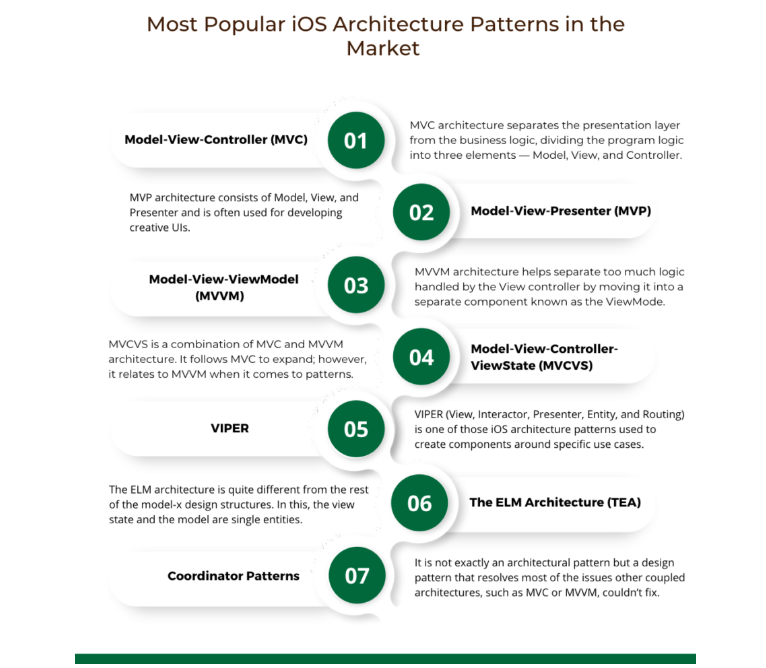
\includegraphics[width=0.8\textwidth]{images/mohinhkientrucios.png}
     \caption{Một số mô hình kiến trúc IOS\cite{MôHinhIOS}.}
    \label{fig:mohinhkientrucios}
\end{figure}
\subsection{Model–View–Controller (MVC)}
\hspace*{0.8cm}Model–View–Controller (MVC) là một trong những mô hình kiến trúc truyền thống được Apple khuyến nghị sử dụng trong phát triển ứng dụng iOS. Mô hình này chia ứng dụng thành ba thành phần chính với vai trò rõ ràng nhằm tăng tính tổ chức và khả năng bảo trì mã nguồn.
  Thành phần đầu tiên, \textbf{Model}, là nơi quản lý dữ liệu và xử lý logic nghiệp vụ. Tiếp theo, \textbf{View} đảm nhiệm việc hiển thị giao diện người dùng và phản hồi các tương tác từ người dùng. Cuối cùng, \textbf{Controller} đóng vai trò trung gian, liên kết giữa Model và View, đồng thời xử lý các logic điều khiển và điều phối luồng dữ liệu.

  Một số ưu điểm nổi bật của mô hình MVC có thể kể đến như: đây là một mẫu kiến trúc phổ biến, không chỉ trong phát triển ứng dụng iOS mà còn cả trong phát triển web; nó cho phép phân tách rõ ràng trách nhiệm giữa các thành phần, đặc biệt là giữa phía máy chủ và máy khách; và nó rất phù hợp với các ứng dụng nhỏ, đơn giản nhờ tính dễ triển khai.

  Tuy nhiên, đi kèm với những lợi ích đó, MVC cũng tồn tại một số hạn chế. Nhược điểm lớn nhất là tình trạng \textit{"Massive View Controller"}, trong đó Controller trở nên quá lớn và phức tạp khi ứng dụng phát triển. Điều này không chỉ làm giảm khả năng kiểm thử mà còn khiến việc bảo trì trở nên khó khăn hơn do sự phụ thuộc chặt chẽ giữa các thành phần trong kiến trúc.

\subsection{Mô hình MVP trong iOS}

\hspace*{0.8cm}Model-View-Presenter (MVP) là một biến thể của mô hình MVC, với mục đích tách biệt rõ ràng hơn giữa phần hiển thị (View) và logic điều khiển (Presenter). Sự phân tách này giúp tăng khả năng kiểm thử và tái sử dụng mã nguồn, đồng thời nâng cao tính linh hoạt trong việc thay đổi và mở rộng ứng dụng. 

  Thành phần của mô hình MVP gồm ba phần chính: \textbf{Model}, giống như trong mô hình MVC, quản lý dữ liệu và xử lý các logic nghiệp vụ; \textbf{View} là giao diện thụ động, chỉ có nhiệm vụ hiển thị dữ liệu và không tham gia vào việc xử lý logic; \textbf{Presenter} là thành phần xử lý toàn bộ logic nghiệp vụ và đảm nhận vai trò cập nhật dữ liệu cho View.

  Một số ưu điểm của mô hình MVP là: \textit{View} hoàn toàn thụ động, dễ dàng kiểm thử và duy trì; việc xác minh chức năng chính xác của từng thành phần trở nên dễ dàng hơn khi chúng được phân tách rõ ràng; \textit{Presenter} có thể được tái sử dụng với nhiều \textit{View} khác nhau, làm cho mã nguồn trở nên linh hoạt và dễ bảo trì.

  Tuy nhiên, mô hình MVP cũng có một số nhược điểm, bao gồm: sự cần thiết phải viết mã \textit{boilerplate} nhiều; \textit{Presenter} có thể trở nên quá lớn và phức tạp khi ứng dụng phát triển; và cuối cùng, MVP không phổ biến bằng mô hình MVVM trong cộng đồng iOS, làm cho việc tìm kiếm tài liệu và hỗ trợ trở nên khó khăn hơn.

\subsection{Mô hình MVVM trong iOS}

\hspace*{0.8cm}MVVM (Model-View-ViewModel) là một mô hình kiến trúc hiện đại được áp dụng rộng rãi trong phát triển ứng dụng iOS, đặc biệt khi kết hợp với các framework reactive như Combine hoặc RxSwift. Mô hình này giúp tách biệt rõ ràng giữa giao diện người dùng và logic nghiệp vụ, tăng khả năng kiểm thử và dễ bảo trì.

  Mô hình MVVM bao gồm ba thành phần chính: \textbf{Model}, giống như trong các mô hình khác, có nhiệm vụ quản lý dữ liệu và logic nghiệp vụ; \textbf{View}, bao gồm các đối tượng \textbf{UIView} và \textbf{UIViewController}, chịu trách nhiệm hiển thị giao diện người dùng; và \textbf{ViewModel}, thành phần chịu trách nhiệm chuẩn bị dữ liệu từ Model và xử lý logic cần thiết để View có thể hiển thị dữ liệu.

  MVVM có bốn nguyên tắc quan trọng cần tuân thủ: \textbf{The Simplicity Principle} (Nguyên tắc đơn giản) yêu cầu mỗi View chỉ nên có một ViewModel và ngược lại; \textbf{The Blendability Principle} (Nguyên tắc hòa trộn) đề xuất ViewModel cần hỗ trợ tối ưu hóa UI; \textbf{The Designability Principle} (Nguyên tắc thiết kế) nhấn mạnh ViewModel phải cung cấp dữ liệu có thể sử dụng tại thời điểm thiết kế; và \textbf{The Testability Principle} (Nguyên tắc kiểm thử) yêu cầu cả Model và ViewModel phải có khả năng kiểm thử độc lập.

  Ưu điểm của mô hình MVVM bao gồm việc tách biệt rõ ràng các thành phần, dễ dàng kiểm thử (đặc biệt là ViewModel), giảm kích thước và trách nhiệm của ViewController, và hỗ trợ binding dữ liệu giữa View và ViewModel. Tuy nhiên, mô hình này cũng có một số nhược điểm, chẳng hạn như sự phức tạp hơn so với MVC, khả năng dẫn đến "Massive ViewModel" nếu không được tổ chức tốt, và yêu cầu cơ chế binding (thủ công hoặc sử dụng thư viện reactive).

  \subsection{MVCVS (Model-View-Controller-ViewState)}

\hspace*{0.8cm}MVCVS là một sự kết hợp giữa hai kiến trúc MVC và MVVM, giúp tách biệt rõ ràng giữa \textbf{Model}, \textbf{View}, \textbf{Controller}, và \textbf{View State}. Trong mô hình này, \textbf{View State} giữ vai trò quan trọng trong việc theo dõi và cập nhật trạng thái giao diện người dùng.

  Ở giai đoạn \textbf{MVCVS Initialization}, View Controller phải tuân theo Model và View State để khởi tạo các thành phần. Khi có bất kỳ thay đổi nào trong \textbf{Model}, \textbf{MVCVS Model Updates} sẽ cập nhật Document Model và View State. Tiếp theo, trong giai đoạn \textbf{MVCVS View Changes}, View State sẽ phân tích Document View Model và View State, từ đó thực hiện các thay đổi đối với View dựa trên các quan sát. \textbf{MVCVS View State} tách biệt View Controller và View State, nơi View State chịu trách nhiệm cập nhật và lắng nghe các thay đổi trong View. Cuối cùng, \textbf{MVCVS Testability} cho phép kiểm tra logic của View Model và Document Model một cách riêng biệt, giúp việc kiểm thử hiệu quả hơn so với mô hình MVC.

  Về ưu điểm, MVCVS mang lại khả năng quản lý hiệu quả cao và dễ dàng kiểm tra các thành phần riêng biệt nhờ các bài kiểm tra tích hợp. Tuy nhiên, nó cũng có nhược điểm là độ phức tạp cao và khó tiếp cận đối với người mới.

  \subsection{VIPER}

\hspace*{0.8cm}VIPER là một mẫu kiến trúc sạch, được sử dụng khi cần tạo các thành phần xoay quanh các trường hợp sử dụng cụ thể trong iOS. VIPER gồm năm thành phần chính: \textbf{View} (giao diện người dùng), \textbf{Interactor} (logic nghiệp vụ), \textbf{Presenter} (điều phối giữa View và Interactor), \textbf{Entity} (mô hình dữ liệu), và \textbf{Routing} (điều hướng giữa các màn hình).

  Ưu điểm của VIPER là dễ quản lý, đặc biệt khi làm việc với nhóm phát triển lớn. Nó giúp tăng khả năng tái sử dụng mã nguồn, kiểm soát UI và giúp dễ dàng kiểm thử mã nhờ vào việc phân tách các thành phần. Hơn nữa, nó giúp giảm thiểu xung đột hợp nhất mã. Tuy nhiên, VIPER có cấu trúc phức tạp đối với ứng dụng nhỏ, yêu cầu thời gian để làm quen và nhiều lớp trung gian có thể ảnh hưởng đến hiệu suất.

  \subsection{The Elm Architecture (TEA)}

\hspace*{0.8cm}TEA là một mô hình kiến trúc đặc biệt trong iOS, khác biệt so với các cấu trúc Model-X truyền thống. Trạng thái giao diện và mô hình được hợp nhất thành một thực thể duy nhất, và mọi cập nhật được gửi đến thực thể này dưới dạng \textbf{messages} và xử lý thông qua \textbf{reducers}. Dòng sự kiện trong TEA được duy trì theo nguyên lý một chiều (unidirectional), tương tự như Flux hoặc Redux.

  Ưu điểm của TEA là khả năng mô tả View như các hàm thuần túy (pure functions) và thực hiện one-way binding từ Model đến View giúp dễ kiểm soát. Tuy nhiên, TEA cũng có nhược điểm, đó là nó tăng độ phức tạp trong các ứng dụng lớn và không phù hợp với mọi loại ứng dụng.

  \subsection{Coordinator Pattern}

\hspace*{0.8cm}Coordinator không phải là một mẫu kiến trúc chính thức mà là một \textbf{design pattern}, giúp giải quyết các vấn đề điều hướng mà MVC hoặc MVVM không xử lý tốt. Coordinator chịu trách nhiệm tạo và giữ tham chiếu đến ViewController hiện tại, đồng thời thực hiện việc điều hướng giữa các màn hình, như việc hiển thị màn hình mới hoặc đẩy ViewController vào Navigation Controller.

  Một trong những ưu điểm lớn của Coordinator là khả năng tách riêng logic điều hướng, giúp mã dễ bảo trì và tăng tính linh hoạt khi chuyển đổi giữa các màn hình. Tuy nhiên, khi triển khai Coordinator, có thể làm tăng độ phức tạp của ứng dụng, yêu cầu thay đổi cách tiếp cận luồng dữ liệu và không cần thiết cho các ứng dụng nhỏ.
\section{Quản lý trạng thái trong ứng dụng iOS}

Quản lý trạng thái hiệu quả là một phần quan trọng trong kiến trúc ứng dụng iOS, đặc biệt khi ứng dụng phát triển về quy mô và độ phức tạp.

\subsection{Các cách tiếp cận quản lý trạng thái}

Quản lý trạng thái có thể được thực hiện qua nhiều phương pháp khác nhau. Dưới đây là ba cách tiếp cận phổ biến:

\paragraph*{1. Quản lý trạng thái cục bộ:}
Trạng thái có thể được lưu trữ trong ViewController thông qua các thuộc tính của nó. Phương pháp này giúp duy trì sự đơn giản trong các ứng dụng nhỏ và dễ dàng quản lý. Một cách để phản ứng với các thay đổi trạng thái là sử dụng \texttt{Property Observers} với \texttt{didSet}, giúp theo dõi và cập nhật khi trạng thái thay đổi.

\paragraph*{2. Reactive Programming:}
Khi cần sự linh hoạt và tính đồng bộ trong quản lý trạng thái, Reactive Programming là một lựa chọn phổ biến. Apple cung cấp framework reactive chính thức của mình là \textbf{Combine Framework}\cite{Combine-Framework}, hỗ trợ quản lý trạng thái và dòng sự kiện một cách dễ dàng. Bên cạnh đó, \textbf{RxSwift} là thư viện reactive phổ biến trong cộng đồng iOS, giúp quản lý trạng thái và sự kiện trong ứng dụng.

\paragraph*{3. Redux-like Architecture:}
Một cách tiếp cận khác là sử dụng kiến trúc giống Redux, trong đó trạng thái được lưu trữ toàn cục trong một \textbf{Store}. Khi có nhu cầu thay đổi trạng thái, các \textbf{Actions} được gửi để mô tả ý định thay đổi. Các \textbf{Reducers} sau đó sẽ xử lý các Action và trả về trạng thái mới, giúp duy trì tính nhất quán và dễ kiểm soát trong việc quản lý trạng thái toàn cục của ứng dụng.


\subsection{State Containers}

\textbf{The Composable Architecture (TCA)} là một framework được phát triển bởi Point-Free, cung cấp cách tiếp cận có nguyên tắc để xây dựng ứng dụng iOS. Framework này giúp tổ chức mã nguồn một cách rõ ràng và dễ kiểm tra.
Cách thức hoạt động của TCA dựa trên bốn thành phần chính:
\paragraph*{1.State:}
State mô tả trạng thái của một tính năng trong ứng dụng. Mỗi tính năng trong TCA sẽ có một State riêng, giúp quản lý và theo dõi trạng thái dễ dàng.
\paragraph*{2.Action:}
Action là các sự kiện có thể xảy ra trong ứng dụng, chúng mô tả những thay đổi có thể xảy ra đối với trạng thái. Mỗi Action có thể dẫn đến việc thay đổi trạng thái của ứng dụng.
\paragraph*{3.Environment:}
Environment là các dependency cần thiết cho logic của tính năng, như các API hoặc các dịch vụ bên ngoài mà ứng dụng cần để hoạt động. Đây là yếu tố giúp logic trở nên dễ kiểm soát và có thể thay đổi khi cần thiết.
\paragraph*{4.Reducer:}
Reducer xử lý logic và cập nhật trạng thái tương ứng khi có Action xảy ra. Nó nhận vào Action và State hiện tại để tính toán và trả về trạng thái mới.


\section{Quản lý phụ thuộc}
Quản lý phụ thuộc (Dependency Injection - DI) là một kỹ thuật quan trọng để tạo ra mã có thể kiểm thử và bảo trì.

\subsection{Các loại Dependency Injection}

Dependency Injection (DI) là một kỹ thuật thiết kế phần mềm giúp tăng tính linh hoạt và khả năng kiểm thử của ứng dụng. DI cho phép các đối tượng cần các phụ thuộc (dependencies) của chúng được cung cấp từ bên ngoài thay vì tự tạo ra. Có ba loại Dependency Injection phổ biến trong lập trình iOS:

\paragraph*{1. Constructor Injection}
Constructor Injection là một phương pháp cung cấp dependencies thông qua một initializer (hàm khởi tạo) của lớp. Các đối tượng cần phụ thuộc sẽ được truyền vào trong quá trình khởi tạo của lớp, giúp đối tượng có thể sử dụng ngay lập tức những dependencies cần thiết mà không cần phải tự tạo chúng. Phương pháp này giúp đảm bảo rằng các đối tượng luôn được khởi tạo với các giá trị hợp lệ và không có tình trạng thiếu dependencies.

Ví dụ về Constructor Injection:

\begin{lstlisting}[language=Swift]
  class NetworkManager {
      private let apiClient: APIClient
  
      init(apiClient: APIClient) {
          self.apiClient = apiClient
      }
  }
  \end{lstlisting}
  
Trong ví dụ này, NetworkManager nhận một đối tượng APIClient thông qua constructor và sử dụng nó để thực hiện các thao tác mạng. Đây là cách tiếp cận mạnh mẽ vì mọi phụ thuộc đều phải được cung cấp trong khi khởi tạo.
\paragraph*{2. Property Injection}
Property Injection là một phương pháp cung cấp dependencies thông qua các thuộc tính của lớp sau khi đối tượng đã được khởi tạo. Thay vì truyền phụ thuộc vào trong initializer, các dependencies sẽ được gán trực tiếp vào các thuộc tính của đối tượng. Phương pháp này mang lại sự linh hoạt trong việc thay đổi hoặc thay thế các dependencies sau khi đối tượng đã được tạo ra.

Ví dụ về Property Injection:
\begin{lstlisting}[language=Swift]
  class NetworkManager {
    var apiClient: APIClient?
}
  \end{lstlisting}
  Ở đây, apiClient có thể được gán giá trị sau khi một đối tượng NetworkManager đã được khởi tạo. Tuy nhiên, phương pháp này có thể gây khó khăn trong việc đảm bảo rằng đối tượng luôn có tất cả các phụ thuộc cần thiết, vì một số phụ thuộc có thể chưa được gán.

\paragraph*{3. Method Injection}
  Method Injection là một phương pháp cung cấp dependencies cho một phương thức cụ thể. Thay vì cung cấp dependencies ở cấp độ lớp như Constructor Injection hay Property Injection, Method Injection cho phép một phương thức nhận vào dependencies mà nó cần trong khi gọi. Phương pháp này rất hữu ích khi chỉ có một số phương thức cụ thể yêu cầu một phụ thuộc đặc biệt mà không cần phải cung cấp nó cho toàn bộ lớp.

  Ví dụ về Method Injection:
  \begin{lstlisting}[language=Swift]
    class DataManager {
        func fetchData(apiClient: APIClient) {
        }
    }
    \end{lstlisting}
    Ở đây, fetchData nhận một đối tượng APIClient làm tham số và sử dụng nó trong quá trình thực hiện yêu cầu mạng. Điều này giúp đảm bảo rằng APIClient chỉ được cung cấp cho các phương thức cần nó, thay vì phải được lưu trữ trong toàn bộ lớp.
\subsection{DI Containers}
    DI Containers (Dependency Injection Containers) giúp quản lý và cung cấp dependencies một cách tự động và có tổ chức. Thay vì phải tạo đối tượng một cách thủ công và tự mình xử lý tất cả các dependencies, DI Containers cho phép bạn khai báo các phụ thuộc và giải quyết chúng một cách tự động, giúp mã nguồn trở nên dễ duy trì và mở rộng hơn. Một số DI Containers phổ biến trong iOS bao gồm:

    \begin{itemize}
      \item \textbf{Swinject:} Swinject là một DI container phổ biến trong cộng đồng iOS, được viết bằng Swift. Nó cung cấp một cách tiếp cận mạnh mẽ để quản lý dependencies trong các ứng dụng iOS, giúp giảm thiểu sự phụ thuộc trực tiếp giữa các lớp. Swinject hỗ trợ tạo đối tượng tự động và cung cấp các dependencies cho các lớp khác khi cần thiết, đồng thời giúp việc kiểm thử và tái sử dụng mã nguồn trở nên dễ dàng hơn.

      \textbf{Ví dụ về Swinject:}
      \begin{lstlisting}[language=Swift]
        import Swinject

        class NetworkManager {
            func fetchData() {
                print("Fetching data from the network...")
            }
        }

        class ViewController {
            private let networkManager: NetworkManager

            init(networkManager: NetworkManager) {
                self.networkManager = networkManager
            }

            func startFetchingData() {
                networkManager.fetchData()
            }
        }

    let container = Container()
    container.register(NetworkManager.self) { _ in NetworkManager() }
    container.register(ViewController.self) { r in
    ViewController(networkManager: r.resolve(NetworkManager.self)!)
        }

    let viewController = container.resolve(ViewController.self)!
        viewController.startFetchingData()
      \end{lstlisting}
      Trong ví dụ trên, Swinject giúp chúng ta dễ dàng đăng ký và giải quyết dependencies. Container quản lý các đối tượng và tự động cung cấp chúng khi yêu cầu.

      \item \textbf{Service Locator:} Service Locator là một giải pháp thay thế cho Dependency Injection. Thay vì truyền dependencies qua constructor hoặc các phương thức, Service Locator cung cấp một trung tâm quản lý các dịch vụ, nơi các lớp có thể yêu cầu các dịch vụ khi cần. Mặc dù phương pháp này giảm thiểu sự cần thiết phải truyền dependencies, nhưng nó có thể dẫn đến mã nguồn khó kiểm soát hơn khi số lượng dependencies tăng lên. Do đó, mặc dù Service Locator là một giải pháp đơn giản và dễ triển khai, nhưng nó có thể gây khó khăn trong việc theo dõi sự thay đổi của các dependencies trong ứng dụng lớn.

      \textbf{Ví dụ về Service Locator:}
      \begin{lstlisting}[language=Swift]
        class NetworkManager {
            func fetchData() {
                print("Fetching data from the network...")
            }
        }

        class ServiceLocator {
            static var shared = ServiceLocator()
            private var services = [String: Any]()

            func register<T>(_ service: T) {
                let key = String(describing: T.self)
                services[key] = service
            }

            func resolve<T>() -> T? {
                let key = String(describing: T.self)
                return services[key] as? T
            }
        }


        let networkManager = NetworkManager()
        ServiceLocator.shared.register(networkManager)

        let retrievedNetworkManager = ServiceLocator.shared.resolve() as NetworkManager?
        retrievedNetworkManager?.fetchData()
      \end{lstlisting}
      Trong ví dụ này, Service Locator chịu trách nhiệm quản lý và cung cấp đối tượng `NetworkManager` khi cần thiết. Mặc dù đơn giản, nhưng cách tiếp cận này có thể gây khó khăn trong việc duy trì mã nguồn khi có nhiều dependencies.
    \end{itemize}
    
\section{Cách thiết kế giao diện người dùng}
iOS cung cấp hai framework chính để xây dựng giao diện người dùng: \textbf{UIKit} và \textbf{SwiftUI}.

\subsection{UIKit}
UIKit là framework UI truyền thống cho iOS, sử dụng mô hình lập trình mệnh lệnh và dựa trên lớp:
\begin{itemize}
  \item \textbf{Auto Layout:} Giúp tạo UI thích ứng với các kích thước màn hình khác nhau.
  \item \textbf{View Controller Lifecycle:} Hiểu rõ vòng đời của \textbf{UIViewController} là chìa khóa để quản lý tài nguyên và trạng thái.
  \item \textbf{Reusable Views:} Tái sử dụng views để cải thiện hiệu suất vào khả năng bảo trì.
\end{itemize}

\subsection{SwiftUI}
SwiftUI là framework UI khai báo mới của Apple, giới thiệu từ iOS 13.
\begin{itemize}
  \item \textbf{View Basics:} Sử dụng cấu trúc \texttt{protocol View} để xây dựng UI.
  \item \textbf{State và Binding:} Sử dụng \texttt{property wrappers} để quản lý trạng thái.
  \item \textbf{ObservableObject và EnvironmentObject:} Cung cấp các cơ chế để quản lý trạng thái phức tạp.
\end{itemize}

\subsection{So sánh UIKit và SwiftUI}

\begin{center}
\begin{tabular}{|l|l|l|}
\hline
\textbf{Khía cạnh} & \textbf{UIKit} & \textbf{SwiftUI} \\
\hline
Năm ra mắt & 2008 & 2019 \\
\hline
Loại lập trình & Mệnh lệnh & Khai báo \\
\hline
Cấu trúc & Dựa trên lớp (Class-based) & Dựa trên struct (Struct-based) \\
\hline
Trạng thái & Tự quản lý & Property wrappers \\
\hline
Hỗ trợ iOS & iOS 2+ & iOS 13+ \\
\hline
Độ ổn định & Rất ổn định & Đang phát triển \\
\hline
Học tập & Phức tạp & Dễ dàng hơn \\
\hline
Tùy biến & Rất linh hoạt & Hạn chế hơn \\
\hline
\end{tabular}
\end{center}

\section{Xử lý Dữ liệu}

Quản lý dữ liệu là một phần quan trọng trong phát triển ứng dụng iOS. Apple cung cấp nhiều giải pháp khác nhau để lưu trữ và truy xuất dữ liệu, phù hợp với các mục đích và quy mô sử dụng khác nhau. Dưới đây là so sánh và mô tả chi tiết các giải pháp lưu trữ dữ liệu phổ biến trong hệ sinh thái iOS.


\subsection{Core Data}
Core Data\cite{Core-Data} là một framework của Apple được thiết kế để quản lý graph đối tượng và vòng đời dữ liệu trong ứng dụng iOS, không phải là một cơ sở dữ liệu thuần túy. Nó cung cấp một cách tiếp cận mạnh mẽ để làm việc với dữ liệu có cấu trúc phức tạp và lưu trữ trong các ứng dụng iOS.

\textbf{Kiến trúc Core Data} bao gồm một số thành phần quan trọng. Đầu tiên là \textbf{NSManagedObjectModel}, mô tả cấu trúc của các entities, attributes và relationships trong ứng dụng. \textbf{NSManagedObjectContext} là không gian làm việc để thực hiện các thao tác CRUD (Create, Read, Update, Delete), trong khi \textbf{NSPersistentStoreCoordinator} điều phối giữa object model và persistent store. Đối với các ứng dụng từ iOS 10 trở lên, \textbf{NSPersistentContainer} cung cấp một cách dễ dàng để đóng gói toàn bộ stack Core Data, giúp đơn giản hóa việc cấu hình và quản lý dữ liệu. Để truy vấn dữ liệu, \textbf{NSFetchRequest} được sử dụng để lấy dữ liệu từ persistent store.

Core Data cung cấp một số \textbf{đặc điểm chính}, bao gồm khả năng quản lý object graph và các mối quan hệ phức tạp, lưu trữ dữ liệu thông qua SQLite backend, và hỗ trợ tính năng tải dữ liệu một cách lười biếng (lazy loading). Hệ thống còn tích hợp kiểm tra dữ liệu và hỗ trợ migration/versioning, giúp dễ dàng cập nhật và bảo trì dữ liệu qua các phiên bản ứng dụng khác nhau.

Về \textbf{ưu điểm}, Core Data tích hợp chặt chẽ với hệ sinh thái của Apple, bao gồm các công cụ thiết kế mô hình dữ liệu trực quan. Nó còn hỗ trợ đồng bộ hóa dữ liệu với CloudKit và có khả năng quản lý bộ nhớ thông minh, tối ưu hóa việc sử dụng tài nguyên.
Tuy nhiên, Core Data cũng có \textbf{nhược điểm}. Đường cong học tập của nó khá dốc, khiến người mới làm quen cảm thấy khó khăn trong việc sử dụng. Việc debug cũng trở nên phức tạp và khó khăn, và Core Data không hoàn toàn thread-safe, điều này có thể gây ra các vấn đề khi thao tác với dữ liệu từ nhiều luồng cùng lúc.

Cuối cùng, \textbf{Core Data} là sự lựa chọn lý tưởng cho các ứng dụng có dữ liệu phức tạp và nhiều quan hệ. Nó cũng rất phù hợp cho các dự án dài hạn cần bảo trì tốt và dễ dàng cập nhật dữ liệu trong suốt vòng đời phát triển.

\subsection{Realm}
Realm là một cơ sở dữ liệu di động mã nguồn mở được thiết kế để thay thế Core Data với hiệu suất cao và API đơn giản, giúp các nhà phát triển dễ dàng xây dựng ứng dụng với dữ liệu lưu trữ hiệu quả. Đặc biệt, Realm cung cấp một số tính năng nổi bật, làm cho nó trở thành một lựa chọn hấp dẫn trong việc quản lý dữ liệu cho các ứng dụng di động.

\textbf{Đặc điểm chính} của Realm bao gồm khả năng hoạt động đa nền tảng, hỗ trợ cả iOS và Android, giúp các nhà phát triển xây dựng ứng dụng cross-platform dễ dàng hơn. Một tính năng quan trọng khác của Realm là kiến trúc "zero-copy", cho phép truy cập dữ liệu trực tiếp mà không cần sao chép bộ nhớ, mang lại hiệu suất cao. Realm cũng hỗ trợ lập trình reactive, giúp đơn giản hóa việc xử lý các thay đổi dữ liệu và cập nhật UI trong ứng dụng. Một điểm mạnh khác của Realm là tính năng thread-safe theo từng instance của Realm, đảm bảo dữ liệu an toàn khi truy cập từ nhiều luồng khác nhau. Nó còn hỗ trợ mã hóa và đồng bộ hóa dữ liệu thời gian thực, mang lại sự linh hoạt cho các ứng dụng yêu cầu tính năng đồng bộ cao.

\textbf{Ưu điểm} của Realm là API đơn giản và dễ học, giúp tiết kiệm thời gian cho các nhà phát triển khi tích hợp vào ứng dụng. Ngoài ra, hiệu suất của Realm rất cao, điều này rất quan trọng đối với các ứng dụng cần xử lý lượng dữ liệu lớn. Realm còn hỗ trợ đồng bộ hóa dữ liệu theo thời gian thực, một tính năng cần thiết trong các ứng dụng cần cập nhật dữ liệu liên tục. Tài liệu của Realm rất rõ ràng và dễ tiếp cận, cùng với cộng đồng lớn và nhiệt tình hỗ trợ, giúp nhà phát triển giải quyết các vấn đề nhanh chóng.
Mặc dù có nhiều ưu điểm, \textbf{Realm} cũng có \textbf{nhược điểm}. Đầu tiên, Realm không tích hợp sâu với iOS, điều này có thể gây khó khăn khi tích hợp với các framework khác của Apple. Thứ hai, Realm không hỗ trợ struct, thay vào đó yêu cầu sử dụng class kế thừa từ \texttt{Object}, điều này có thể gây ra một số bất tiện cho các nhà phát triển. Thêm vào đó, một số giới hạn trong model threading và truy vấn phức tạp có thể ảnh hưởng đến tính linh hoạt của ứng dụng khi xử lý các tình huống dữ liệu phức tạp.

Về \textbf{khi nên dùng}, Realm là sự lựa chọn tuyệt vời cho các ứng dụng cross-platform, giúp dễ dàng triển khai trên cả iOS và Android mà không gặp phải vấn đề tương thích. Nó cũng rất thích hợp cho các dự án yêu cầu hiệu suất cao và đồng bộ hóa dữ liệu theo thời gian thực, ví dụ như các ứng dụng cần tính năng đồng bộ dữ liệu giữa các thiết bị. Cuối cùng, Realm rất phù hợp cho các dự án ưu tiên offline-first, khi ứng dụng cần có khả năng hoạt động tốt mà không phụ thuộc quá nhiều vào kết nối mạng.

\subsection{SQLite}
SQLite là một hệ quản trị cơ sở dữ liệu quan hệ nhỏ gọn, không yêu cầu server và được sử dụng rộng rãi trên thế giới nhờ vào sự đơn giản, hiệu quả và dễ triển khai. Với thiết kế "self-contained", SQLite không cần cài đặt riêng biệt hoặc máy chủ, khiến nó trở thành một lựa chọn phổ biến cho các ứng dụng di động và ứng dụng nhúng.

\textbf{Đặc điểm chính} của SQLite là tính tự chứa và không yêu cầu cấu hình, giúp dễ dàng tích hợp vào các ứng dụng mà không gặp phải những phức tạp của việc cài đặt và cấu hình server. SQLite rất nhẹ và đáng tin cậy, đồng thời hỗ trợ đa nền tảng (cross-platform), có thể chạy trên nhiều hệ điều hành khác nhau. SQLite hỗ trợ đầy đủ SQL, cho phép thực hiện các thao tác truy vấn cơ sở dữ liệu mạnh mẽ và linh hoạt. Hệ thống này tuân thủ chuẩn ACID, đảm bảo các thao tác dữ liệu được thực hiện một cách an toàn và chính xác, ngay cả khi hệ thống gặp sự cố.

\textbf{Ưu điểm} của SQLite là khả năng kiểm soát toàn diện schema và truy vấn. Điều này có nghĩa là bạn có thể hoàn toàn tùy chỉnh cấu trúc dữ liệu và các câu truy vấn theo nhu cầu của ứng dụng. SQLite cũng rất phù hợp với các truy vấn phức tạp nhờ vào tính mạnh mẽ của SQL. Ngoài ra, SQLite rất dễ dàng để sao lưu và khôi phục, một yếu tố quan trọng trong việc bảo vệ dữ liệu của ứng dụng.

Tuy nhiên, \textbf{SQLite} cũng có \textbf{nhược điểm}. Một trong những khó khăn là bạn phải tự xử lý các vấn đề về thread-safe và migration, vì SQLite không cung cấp các công cụ tự động hóa cho những vấn đề này. SQLite cũng không hỗ trợ object mapping tự động, điều này có thể khiến việc làm việc với các đối tượng trong ứng dụng trở nên phức tạp hơn. Cuối cùng, SQLite không phải là công cụ lý tưởng cho các ứng dụng sử dụng mô hình lập trình reactive, vì nó không hỗ trợ cập nhật dữ liệu theo thời gian thực một cách tự động.

Về \textbf{khi nên dùng}, SQLite là lựa chọn lý tưởng nếu bạn cần kiểm soát hoàn toàn cơ sở dữ liệu và muốn thực hiện các thao tác SQL phức tạp. Nó cũng phù hợp với các ứng dụng không yêu cầu tích hợp chặt với hệ sinh thái iOS, ví dụ như các ứng dụng nhỏ hoặc nhúng, nơi cần sự đơn giản và hiệu suất cao.

\subsection{UserDefaults}
\textbf{Định nghĩa:} \texttt{UserDefaults} là một hệ thống lưu trữ key-value đơn giản, được thiết kế để lưu trữ dữ liệu nhỏ và không nhạy cảm. Đây là công cụ lý tưởng cho việc lưu trữ các cài đặt hoặc trạng thái người dùng trong ứng dụng iOS.

\textbf{Đặc điểm chính:} \texttt{UserDefaults} hỗ trợ lưu trữ dữ liệu dưới dạng key-value. Với API đơn giản, nó cho phép lưu trữ các kiểu cơ bản như String, Int, Bool, Date, và các đối tượng đơn giản khác. Hệ thống này tự động đồng bộ hóa và có cache nội bộ, đồng thời có khả năng đồng bộ với iCloud, cho phép dữ liệu người dùng được lưu trữ và truy cập trên nhiều thiết bị Apple.

\textbf{Ưu điểm:} Với \texttt{UserDefaults}, việc lưu trữ dữ liệu trở nên dễ dàng và hiệu quả. Nó có hiệu suất cao khi lưu trữ các dữ liệu nhỏ và không yêu cầu cấu hình phức tạp. \texttt{UserDefaults} rất thích hợp để lưu trữ trạng thái người dùng hoặc các cài đặt của ứng dụng.

\textbf{Nhược điểm:} Mặc dù dễ sử dụng, \texttt{UserDefaults} không phù hợp cho việc lưu trữ dữ liệu lớn hoặc nhạy cảm vì thiếu các tính năng bảo mật. Thêm vào đó, nó không hỗ trợ các thao tác phức tạp như lọc, truy vấn, hoặc giao dịch dữ liệu, điều này có thể hạn chế trong các ứng dụng cần thao tác với dữ liệu phức tạp.

\textbf{Khi nên dùng:} \texttt{UserDefaults} là lựa chọn lý tưởng khi bạn cần lưu trữ các thông tin đơn giản như theme, ngôn ngữ, âm thanh, hoặc đánh dấu các trạng thái hoàn thành, như đã hoàn thành hướng dẫn sử dụng. Nó cũng rất phù hợp cho việc lưu các cấu hình đơn giản hoặc flags trong ứng dụng.

\subsection{Keychain}
\textbf{Định nghĩa:} \texttt{Keychain} là hệ thống lưu trữ an toàn được thiết kế để bảo vệ thông tin nhạy cảm như mật khẩu, token xác thực và các dữ liệu quan trọng khác. Hệ thống này đảm bảo rằng dữ liệu được mã hóa và chỉ có thể truy cập thông qua các phương thức bảo mật.

\textbf{Đặc điểm chính:} \texttt{Keychain} lưu trữ dữ liệu với mã hóa mạnh mẽ, giúp bảo vệ thông tin nhạy cảm khỏi các mối đe dọa bên ngoài. Dữ liệu trong \texttt{Keychain} tồn tại lâu dài, ngay cả khi ứng dụng bị xóa. Nó hỗ trợ xác thực sinh trắc học như Face ID và Touch ID, đồng thời có thể chia sẻ giữa các ứng dụng của cùng một nhà phát triển. \texttt{Keychain} cũng hỗ trợ đồng bộ hóa với iCloud, cho phép người dùng truy cập dữ liệu bảo mật trên nhiều thiết bị Apple.

\textbf{Ưu điểm:} Một trong những ưu điểm chính của \texttt{Keychain} là mức độ bảo mật cao, làm cho nó trở thành lựa chọn lý tưởng cho việc lưu trữ các thông tin nhạy cảm. Hệ thống này hỗ trợ xác thực bằng Face ID và Touch ID, cung cấp một lớp bảo vệ thêm cho dữ liệu. Hơn nữa, dữ liệu trong \texttt{Keychain} tồn tại lâu dài và có thể được sử dụng trên nhiều thiết bị.

\textbf{Nhược điểm:} Tuy nhiên, \texttt{Keychain} cũng có một số hạn chế. API của nó phức tạp và khó sử dụng hơn so với các giải pháp lưu trữ thông thường, đòi hỏi người phát triển phải có kiến thức chuyên sâu. Thêm vào đó, việc truy cập và thao tác dữ liệu trong \texttt{Keychain} thường chậm hơn so với lưu trữ thông thường. Cuối cùng, việc debug và kiểm tra dữ liệu trong \texttt{Keychain} cũng gặp khó khăn do tính bảo mật cao.

\textbf{Khi nên dùng:} \texttt{Keychain} là giải pháp lý tưởng khi bạn cần lưu trữ các thông tin nhạy cảm như mật khẩu, token xác thực, hoặc các thông tin bảo mật khác. Nó rất phù hợp cho những ứng dụng có yêu cầu bảo mật cao, nơi mà việc đảm bảo an toàn dữ liệu người dùng là ưu tiên hàng đầu.
\section{Xử lý bất đồng bộ}

Xử lý tác vụ bất đồng bộ là một phần thiết yếu trong kiến trúc ứng dụng iOS hiện đại, giúp đảm bảo giao diện người dùng mượt mà và phản hồi tốt. Swift cung cấp nhiều phương pháp để xử lý bất đồng bộ, từ truyền thống đến hiện đại, mỗi phương pháp có ưu và nhược điểm riêng phù hợp với từng hoàn cảnh.

\subsection{Completion Handlers}
\textbf{Định nghĩa:} Completion handlers là cơ chế truyền thống trong iOS để xử lý các tác vụ bất đồng bộ, trong đó closures được sử dụng để thông báo khi một tác vụ hoàn thành. Khi hàm bất đồng bộ hoàn thành, closure sẽ được gọi để tiếp tục xử lý.

\textbf{Cơ chế hoạt động:} Một hàm bất đồng bộ trong iOS sẽ nhận một closure làm tham số. Closure này được gọi khi tác vụ bất đồng bộ kết thúc, cho phép người phát triển thực hiện các hành động tiếp theo. Thường thì, kiểu dữ liệu \texttt{Result} được sử dụng để phân biệt giữa thành công và thất bại của tác vụ, giúp việc xử lý lỗi và kết quả trở nên rõ ràng hơn.

\textbf{Ưu điểm:} Completion handlers rất dễ hiểu và sử dụng rộng rãi trong cộng đồng lập trình iOS. Không cần phải cài đặt thêm thư viện bên ngoài, việc sử dụng closure giúp tiết kiệm thời gian và đơn giản hóa mã nguồn. Ngoài ra, completion handlers tương thích với tất cả các phiên bản iOS, không yêu cầu tính năng đặc biệt.

\textbf{Nhược điểm:} Tuy nhiên, việc sử dụng completion handlers cũng gặp phải một số vấn đề. Khi chuỗi nhiều tác vụ bất đồng bộ được gọi, rất dễ rơi vào tình trạng \textit{callback hell}, nơi mã trở nên khó hiểu và khó bảo trì. Thêm vào đó, việc truyền lỗi giữa các callback có thể gặp khó khăn, và nếu không cẩn thận, việc quên gọi completion handler có thể gây lỗi trong ứng dụng. Hơn nữa, khi cần thực hiện các tác vụ song song hoặc tuần tự một cách tối ưu, completion handlers có thể không phải là giải pháp hiệu quả nhất.

\subsection{Promises}
\textbf{Định nghĩa:} Promises là một mô hình xử lý bất đồng bộ dựa trên hướng đối tượng, giúp các tác vụ bất đồng bộ được thực hiện tuần tự và dễ dàng quản lý. Mô hình này thường được sử dụng thông qua các thư viện như \texttt{PromiseKit} trong iOS, và nó cung cấp một cách tiếp cận rõ ràng hơn so với completion handlers truyền thống.

\textbf{Cơ chế hoạt động:} Một \texttt{Promise} đại diện cho kết quả sẽ có trong tương lai, giúp mã nguồn dễ hiểu hơn khi xử lý bất đồng bộ. Để xử lý kết quả, ta sử dụng \texttt{.then}, cho phép tiếp tục chuỗi các tác vụ bất đồng bộ. Khi có lỗi xảy ra, \texttt{.catch} sẽ giúp xử lý lỗi một cách tập trung, thay vì phải làm điều này ở nhiều nơi trong mã nguồn. Mô hình Promise cũng dễ dàng kết hợp và biến đổi, giúp việc quản lý các tác vụ bất đồng bộ trở nên thuận tiện và linh hoạt hơn.

\textbf{Ưu điểm:} Promises cung cấp cú pháp rõ ràng và dễ hiểu, đặc biệt là giúp tránh tình trạng \textit{callback hell} khi chuỗi các tác vụ trở nên dài và phức tạp. Chúng hỗ trợ thực hiện các tác vụ song song hoặc tuần tự một cách dễ dàng và hiệu quả, đồng thời quản lý lỗi tập trung, giúp mã nguồn trở nên gọn gàng hơn. Hơn nữa, Promises hỗ trợ chaining (nối tiếp các tác vụ) và transform (biến đổi) dữ liệu, cho phép tạo ra các chuỗi bất đồng bộ phức tạp một cách mượt mà.

\textbf{Nhược điểm:} Tuy nhiên, Promises yêu cầu cài đặt các thư viện bên thứ ba như \texttt{PromiseKit}, điều này có thể làm tăng độ phức tạp của dự án ban đầu. Ngoài ra, mặc dù Promises giúp đơn giản hóa mã nguồn về lâu dài, nhưng người lập trình có thể cần thời gian để làm quen với mô hình này. Cuối cùng, việc debug mã sử dụng Promises có thể khó khăn hơn so với mã đồng bộ truyền thống, do các kết quả và lỗi được xử lý sau khi tác vụ hoàn thành.
\subsection{Async/Await}
\textbf{Định nghĩa:} Từ iOS 15 trở đi, Swift hỗ trợ cú pháp \texttt{async/await}, một mô hình mới cho phép viết mã bất đồng bộ theo cách dễ đọc và dễ quản lý hơn, giống như code đồng bộ truyền thống. Với \texttt{async/await}, mã bất đồng bộ không còn cần đến các callback hoặc closure phức tạp, giúp cải thiện khả năng duy trì và mở rộng ứng dụng.

\textbf{Cơ chế hoạt động:} Cú pháp \texttt{async} được sử dụng để đánh dấu một hàm là bất đồng bộ, trong khi \texttt{await} giúp tạm dừng thực thi của hàm cho đến khi có kết quả trả về. Điều này cho phép viết mã theo kiểu tuần tự mà không bị chặn lại bởi các tác vụ bất đồng bộ. Swift cũng hỗ trợ cấu trúc concurrency rõ ràng thông qua \texttt{Task} và \texttt{TaskGroup}, giúp dễ dàng quản lý và tổ chức các tác vụ đồng thời. Mô hình này cũng dễ dàng kết hợp với \texttt{try-catch} để xử lý lỗi, giúp mã nguồn trở nên mượt mà và dễ đọc hơn.

\textbf{Ưu điểm:} Cú pháp \texttt{async/await} giúp mã nguồn trở nên gọn gàng, dễ đọc và dễ duy trì, đặc biệt khi so với các mô hình callback truyền thống. Quản lý luồng logic và xử lý lỗi trở nên tự nhiên và trực quan hơn, do không cần phải lồng nhiều closure vào nhau. Hơn nữa, cú pháp này tích hợp sâu vào hệ sinh thái của Apple, từ iOS, macOS đến các dịch vụ như CloudKit và URLSession, giúp lập trình viên dễ dàng tiếp cận và sử dụng.

\textbf{Nhược điểm:} Một nhược điểm lớn của cú pháp \texttt{async/await} là yêu cầu phiên bản iOS 15 trở lên, điều này có thể gây khó khăn khi phát triển ứng dụng cần hỗ trợ các phiên bản cũ hơn. Thêm vào đó, để tận dụng được lợi ích của \texttt{async/await}, có thể cần phải refactor lại call stack của các hàm, điều này có thể mất thời gian. Cuối cùng, nếu không quản lý cẩn thận việc hủy các tác vụ bằng \texttt{Task.cancel()}, có thể gây ra vấn đề rò rỉ bộ nhớ.
\subsection{Combine Framework}
\textbf{Định nghĩa:} Combine là một framework lập trình reactive được Apple phát triển, ra mắt từ iOS 13, nhằm hỗ trợ xử lý bất đồng bộ dựa trên dữ liệu và sự kiện. Combine cung cấp một cách tiếp cận hiệu quả để xử lý các luồng dữ liệu và sự kiện trong ứng dụng, giúp lập trình viên có thể dễ dàng quản lý và biến đổi dữ liệu theo cách thức phản ứng với các thay đổi.

\textbf{Cơ chế hoạt động:} Combine dựa trên mô hình \textit{Publisher/Subscriber}, trong đó \texttt{Publisher} phát ra giá trị, và \texttt{Subscriber} nhận và xử lý những giá trị này. Lập trình viên có thể tạo ra các chuỗi pipeline để xử lý và biến đổi dữ liệu, bao gồm việc lọc, kết hợp, hoặc áp dụng các phép toán phức tạp lên dữ liệu. Framework này hỗ trợ việc quản lý backpressure, giúp đảm bảo rằng hệ thống không bị quá tải bởi các sự kiện đến quá nhanh. Combine kết hợp mạnh mẽ với \texttt{SwiftUI}, cho phép xây dựng giao diện người dùng động và phản ứng với các thay đổi trong dữ liệu.

\textbf{Ưu điểm:} Một trong những ưu điểm lớn của Combine là khả năng tích hợp chặt chẽ với Swift và toàn bộ hệ sinh thái Apple, làm cho việc xây dựng ứng dụng trở nên liền mạch và hiệu quả. Framework cung cấp hàng trăm operators hỗ trợ biến đổi và lọc dữ liệu, giúp lập trình viên có thể thực hiện các tác vụ phức tạp một cách dễ dàng. Ngoài ra, Combine tự động quản lý bộ nhớ thông qua \texttt{AnyCancellable}, giúp giảm bớt nỗi lo về việc giải phóng tài nguyên. Combine cho phép xử lý đồng bộ và bất đồng bộ một cách nhất quán, giúp quản lý dữ liệu và sự kiện một cách hiệu quả.

\textbf{Nhược điểm:} Một nhược điểm của Combine là learning curve khá cao, yêu cầu lập trình viên phải hiểu rõ về lập trình reactive và các khái niệm liên quan. Thêm vào đó, Combine yêu cầu iOS 13 trở lên, điều này có thể hạn chế việc sử dụng trong các ứng dụng cần hỗ trợ các phiên bản iOS cũ hơn. Việc debugging các pipeline phức tạp cũng có thể gặp khó khăn, đặc biệt khi chuỗi các phép toán trở nên dài và khó theo dõi. Cuối cùng, mặc dù Combine mạnh mẽ, nhưng nó không hỗ trợ đa nền tảng như \texttt{RxSwift}, điều này có thể là một hạn chế nếu bạn muốn phát triển ứng dụng trên nhiều nền tảng.
\section{Kết luận}

Trong kiến trúc ứng dụng iOS hiện đại, không chỉ có sự phân tách rõ ràng giữa các tầng chức năng như UI, Business Logic và Data, mà còn chú trọng đến khả năng mở rộng, dễ bảo trì và hiệu suất của ứng dụng. Mục tiêu này đạt được thông qua việc áp dụng các mô hình kiến trúc như MVC, MVVM, VIPER, kết hợp với các kỹ thuật xử lý bất đồng bộ hiện đại như \texttt{Completion Handlers}, \texttt{Promises}, \texttt{Async/Await}, và \texttt{Combine}. Những kỹ thuật này giúp xây dựng ứng dụng mượt mà, linh hoạt và thân thiện với người dùng.

\vspace{0.5em}

Mỗi cách tiếp cận này đều có những ưu và nhược điểm riêng, vì vậy, việc lựa chọn phương pháp phù hợp cần dựa trên yêu cầu của dự án và phiên bản iOS mà ứng dụng hỗ trợ. Cụ thể:

\begin{itemize}
\item \textbf{Completion Handlers} vẫn là lựa chọn đơn giản và phổ biến, nhờ vào tính linh hoạt và dễ hiểu.
\item \textbf{Promises} mang lại cú pháp rõ ràng hơn cho các chuỗi bất đồng bộ, giúp mã nguồn dễ theo dõi và bảo trì.
\item \textbf{Async/Await} đang dần trở thành tiêu chuẩn mới nhờ vào sự rõ ràng và tích hợp sâu trong ngôn ngữ Swift, đồng thời cải thiện khả năng đọc hiểu mã nguồn.
\item \textbf{Combine} mở ra hướng lập trình phản ứng hiện đại, đặc biệt phù hợp với các ứng dụng yêu cầu nhiều tương tác và dữ liệu động.
\end{itemize}

Việc lựa chọn kiến trúc và công nghệ phù hợp không chỉ giúp tối ưu hóa hiệu suất mà còn tạo ra trải nghiệm người dùng vượt trội. Trong bối cảnh hệ sinh thái Apple không ngừng phát triển, việc nắm vững và ứng dụng linh hoạt các kỹ thuật hiện đại sẽ là chìa khóa giúp các nhà phát triển iOS tạo ra những sản phẩm thành công và bền vững.






\chapter{Kiến trúc đa nền tảng}
\label{chap:Chap4}

\section{Giới thiệu}
  
    \hspace*{0.8cm}Trong bối cảnh số lượng người dùng thiết bị di động không ngừng tăng, nhu cầu phát triển ứng dụng hoạt động mượt mà trên cả iOS và Android ngày càng trở nên cấp thiết. Kiến trúc đa nền tảng (cross-platform) đã nổi lên như một giải pháp giúp doanh nghiệp tối ưu chi phí, rút ngắn thời gian phát hành và đơn giản hóa quy trình bảo trì so với phương pháp native truyền thống. Các framework như React Native và Flutter cho phép tái sử dụng 50--80\% mã nguồn, đồng thời cung cấp công cụ phát triển hiện đại như hot reload và bộ widget tùy biến cao. Nghiên cứu này tập trung phân tích ưu nhược điểm của hai framework trên qua các khía cạnh: hiệu năng (FPS, RAM), chi phí, thời gian triển khai và khả năng ứng dụng vào các loại dự án khác nhau, từ đó đề xuất tiêu chí lựa chọn phù hợp cho từng trường hợp sử dụng cụ thể.  
\vspace{0.5em}

\subsection{Bối cảnh nghiên cứu}
\renewcommand{\labelitemi}{--}    

    \hspace*{0.8cm}Sự phát triển nhanh chóng của thị trường di động trong những năm gần đây đã làm thay đổi đáng kể cách thức xây dựng ứng dụng. Theo báo cáo của Statista (2023)~\cite{statista2023}, số lượng người dùng smartphone toàn cầu đạt 6.92 tỷ vào năm 2023 và dự kiến sẽ tăng lên 7.5 tỷ vào năm 2025. Trước thực tế này, các nhà phát triển đứng trước bài toán lớn: làm thế nào để tạo ra ứng dụng chạy trơn tru trên cả iOS và Android mà không cần xây dựng hai hệ thống riêng biệt?
\vspace{0.5em}


    \hspace*{0.8cm}Phát triển ứng dụng native cho từng nền tảng từng là giải pháp phổ biến, nhưng nó kéo theo chi phí cao, thời gian dài và yêu cầu nguồn nhân lực lớn. Ví dụ, một công ty startup có thể mất tới 18 tháng và khoảng 500.000 USD để xây dựng song song hai ứng dụng native cho iOS và Android.
\vspace{0.5em}


    \hspace*{0.8cm}Chỉ riêng chi phí nhân sự đã là gánh nặng: theo Business of Apps~\cite{businessofapps2025}, mức lương trung bình hàng năm của lập trình viên ứng dụng di động tại Mỹ dao động từ 80.000 đến 150.000 USD, tùy thuộc vào công nghệ và kinh nghiệm. Ví dụ, lập trình viên Flutter có thể nhận khoảng 7.800 USD/tháng, trong khi React Native là khoảng 8.000 USD/tháng. Với hai lập trình viên làm việc trong 18 tháng, tổng chi phí nhân sự có thể lên đến 280.000--350.000 USD, chưa kể đến chi phí thiết kế, kiểm thử và quản lý dự án.
\vspace{0.5em}


    \hspace*{0.8cm}Để giải quyết những hạn chế này, các công nghệ phát triển ứng dụng đa nền tảng (cross-platform) bắt đầu nổi lên như một giải pháp tiềm năng. Kể từ khi Facebook giới thiệu React Native vào năm 2015, lập trình viên đã có thể sử dụng JavaScript để viết giao diện và logic nghiệp vụ, từ đó giảm thiểu đáng kể lượng mã cần viết riêng cho từng hệ điều hành. Tiếp đó, năm 2017, Google ra mắt Flutter, framework sử dụng ngôn ngữ Dart và engine Skia, cho phép render UI trực tiếp mà không phụ thuộc vào widget native.
\vspace{0.5em}


    \hspace*{0.8cm}Nhờ khả năng tái sử dụng mã nguồn lên tới 50--80\% giữa hai nền tảng, giải pháp cross-platform giúp các startup cắt giảm 30--40\% chi phí phát triển so với native thuần túy. Báo cáo của Cleveroad~\cite{cleveroad} cũng ghi nhận rằng, chi phí phát triển ứng dụng đa nền tảng thường dao động từ 60.000--200.000 USD, thấp hơn đáng kể so với mức 70.000--250.000 USD nếu phát triển từng ứng dụng riêng biệt. Không chỉ tiết kiệm ngân sách, thời gian đưa sản phẩm ra thị trường cũng được rút ngắn nhờ sử dụng chung codebase và quy trình kiểm thử tập trung. Ví dụ, một ứng dụng phức tạp thường mất 7--16 tuần để phát triển native độc lập, nhưng chỉ cần 11--20 tuần với React Native hoặc Flutter, nhờ tính năng hot reload và workflow thống nhất.
\vspace{0.5em}


    \hspace*{0.8cm}Tổng thể, thay vì mất 18 tháng và 500.000 USD, các công ty hiện nay chỉ cần 12--14 tháng và khoảng 200.000--250.000 USD để hoàn thiện sản phẩm cho cả hai nền tảng, thể hiện rõ ưu thế của các framework cross-platform trong việc tối ưu chi phí và thời gian phát triển.
\vspace{0.5em}


    \hspace*{0.8cm}Theo khảo sát của Stack Overflow (2023)~\cite{stackoverflow2023}, Flutter hiện được 42\% nhà phát triển ưu tiên lựa chọn, trong khi React Native chiếm 38\%. Sự cạnh tranh giữa hai framework này không chỉ phản ánh xu hướng ``Write Once, Run Anywhere'' mà còn đặt ra câu hỏi mới về hiệu năng, khả năng mở rộng và tùy biến trong các ứng dụng hiện đại.
\vspace{0.5em}

\subsection{Mục tiêu nghiên cứu}
\renewcommand{\labelitemi}{--}    

    \hspace*{0.8cm}Bài nghiên cứu này hướng đến ba mục tiêu chính:
    \setlength{\leftmargini}{1.0cm}
    \begin{itemize}
        \item Mục tiêu thứ nhất là phân tích ưu điểm và hạn chế của kiến trúc đa nền tảng so với phát triển native, nhằm đánh giá khả năng tiết kiệm chi phí, rút ngắn thời gian phát triển, đồng thời nhận diện các thách thức liên quan đến hiệu năng và trải nghiệm người dùng.
        \item Mục tiêu thứ hai là đo lường và phân tích các rào cản về mặt kỹ thuật của ứng dụng đa nền tảng, thông qua các chỉ số như tốc độ khung hình (FPS), mức tiêu thụ RAM, và thời gian phản hồi. Từ đó, so sánh các giá trị này với ứng dụng native để xác định mức độ chênh lệch rõ ràng.
        \item Mục tiêu thứ ba là đề xuất tiêu chí lựa chọn framework phù hợp với từng loại dự án, dựa trên ngân sách, thời gian triển khai và đặc thù ứng dụng. Ví dụ, Flutter có thể phù hợp với ứng dụng thiên về đồ họa như game, trong khi React Native có thể là lựa chọn tối ưu cho ứng dụng doanh nghiệp.
    \end{itemize}
\vspace{0.5em}

\subsection{Phạm vi và đối tượng}
\renewcommand{\labelitemi}{--}    

    \hspace*{0.8cm}Phạm vi nghiên cứu tập trung vào hai framework hàng đầu trong phát triển ứng dụng đa nền tảng hiện nay, bao gồm:
    \setlength{\leftmargini}{1.0cm}
    \begin{itemize}
        \item \textbf{React Native}, do Facebook phát triển, dựa trên ngôn ngữ JavaScript. Framework này nổi bật nhờ hệ sinh thái mở rộng (npm, Expo) và khả năng tích hợp dễ dàng vào các hệ thống web sẵn có.
        \item \textbf{Flutter}, do Google phát triển, sử dụng ngôn ngữ Dart. Framework này được đánh giá cao nhờ hiệu năng vượt trội và khả năng tùy biến giao diện người dùng thông qua engine Skia.
    \end{itemize}
\vspace{0.5em}


    \hspace*{0.8cm}Lý do lựa chọn hai framework này đến từ vị thế dẫn đầu thị trường của chúng:
    \setlength{\leftmargini}{1.0cm}
    \begin{itemize}
        \item Theo báo cáo của SlashData (2023)~\cite{slashdata2023}, React Native và Flutter chiếm đến 80\% thị phần framework đa nền tảng.
        \item Cả hai đều sở hữu cộng đồng lập trình viên lớn, tài liệu kỹ thuật phong phú, và đã được triển khai rộng rãi trong các dự án thực tế.
    \end{itemize}
\vspace{0.5em}


    \hspace*{0.8cm}Nguồn dữ liệu trong nghiên cứu được tổng hợp từ các công trình thực nghiệm uy tín:
    \setlength{\leftmargini}{1.0cm}
    \begin{itemize}
        \item \textbf{Nghiên cứu của Wenhao (2018)}~\cite{wenhao2018} tập trung vào đo hiệu năng FPS khi cuộn màn hình trên 10 ứng dụng mẫu. Kết quả cho thấy: \textit{Flutter đạt 60 FPS}, trong khi \textit{React Native đạt 45–50 FPS}.
        \item \textbf{Báo cáo của Biorn-Hansen (2021)}~\cite{biornhansen2021} đánh giá mức tiêu thụ RAM và CPU trên 15 ứng dụng thương mại. Kết quả cho thấy: \textit{Ứng dụng native sử dụng trung bình 150MB RAM}, so với \textit{200MB của Flutter} và \textit{180MB của React Native}.
    \end{itemize}
\vspace{0.5em}


    \hspace*{0.8cm}Giới hạn của nghiên cứu cũng được xác định rõ ràng:
    \setlength{\leftmargini}{1.0cm}
    \begin{itemize}
        \item Các framework ít phổ biến như Xamarin hay Ionic không nằm trong phạm vi phân tích.
        \item Các số liệu hiệu năng được thực hiện trong môi trường thử nghiệm, do đó có thể khác biệt so với khi triển khai thực tế.
    \end{itemize}
\vspace{0.5em}


    \hspace*{0.8cm}Phần giới thiệu khép lại bằng định hướng ứng dụng của nghiên cứu:
    \setlength{\leftmargini}{1.0cm}
    \begin{itemize}
        \item Việc lựa chọn kiến trúc đa nền tảng không chỉ dựa trên công nghệ, mà còn phụ thuộc vào mục tiêu kinh doanh và nguồn lực của doanh nghiệp. Nghiên cứu này hướng đến cung cấp cái nhìn toàn diện về React Native và Flutter, giúp nhà phát triển đưa ra quyết định dựa trên dữ liệu định lượng và phân tích chuyên sâu.
    \end{itemize}
\vspace{0.5em}


\section{Cơ Sở Lý Thuyết }

  Trong quá trình phát triển phần mềm hiện đại, kiến trúc hệ thống đóng vai trò then chốt trong việc đảm bảo hiệu quả và khả năng mở rộng của ứng dụng. Đặc biệt đối với các ứng dụng di động, việc lựa chọn kiến trúc phù hợp có thể ảnh hưởng trực tiếp đến chi phí, thời gian phát triển và trải nghiệm người dùng cuối. Trong phần này, chúng tôi trình bày các khái niệm nền tảng liên quan đến kiến trúc đa nền tảng như một hướng tiếp cận thay thế cho phát triển native truyền thống.
% 2.1
\subsection{Khái niệm kiến trúc đa nền tảng}
\renewcommand{\labelitemi}{--}

\subsubsection{Định nghĩa}

    Kiến trúc đa nền tảng (cross-platform architecture) là một phương pháp phát triển ứng dụng dựa trên một bộ mã nguồn chung, giúp triển khai đồng thời trên nhiều hệ điều hành như iOS, Android, cũng như các nền tảng khác như web hoặc desktop. Thay vì xây dựng từng phiên bản riêng biệt cho từng hệ điều hành, lập trình viên sử dụng các framework hoặc công cụ trung gian để biên dịch mã nguồn và tối ưu hóa cho từng môi trường cụ thể.
\vspace{0.5em}


    Các framework tiêu biểu cho kiến trúc đa nền tảng bao gồm:
    \setlength{\leftmargini}{1.5cm}
    \begin{itemize}
        \item \textbf{React Native}: Sử dụng JavaScript và biên dịch mã qua "bridge" thành mã máy tương ứng (Objective-C/Swift cho iOS, Java/Kotlin cho Android).
        \item \textbf{Flutter}: Dựa trên ngôn ngữ Dart và sử dụng Skia Engine để render giao diện trực tiếp, độc lập với hệ điều hành.
    \end{itemize}

\subsubsection{Nguyên tắc "Write Once, Run Anywhere"-(WORA)}

    Nguyên tắc WORA, được Sun Microsystems giới thiệu từ thập niên 1990, nhấn mạnh vào khả năng tái sử dụng mã nguồn tối đa và giảm chi phí phát triển. Nguyên tắc này dựa trên hai yếu tố cốt lõi:
    \setlength{\leftmargini}{1.5cm}
    \begin{itemize}
        \item \textbf{Tính độc lập nền tảng}: Mã nguồn không bị phụ thuộc vào hệ điều hành hoặc phần cứng cụ thể.
        \item \textbf{Tính nhất quán}: Logic nghiệp vụ và giao diện hoạt động đồng bộ trên mọi thiết bị.
    \end{itemize}
\vspace{0.5em}


    Một số ứng dụng thực tế đã áp dụng hiệu quả nguyên tắc này:
    \setlength{\leftmargini}{1.5cm}
    \begin{itemize}
        \item \textbf{Microsoft Teams}: Dùng React Native để triển khai trên iOS, Android và Windows với hơn 90\% mã nguồn dùng chung.
        \item \textbf{Google Pay}: Xây dựng trên Flutter, hỗ trợ cả mobile và web từ một codebase duy nhất.
    \end{itemize}

\subsubsection{Lợi ích của kiến trúc đa nền tảng}

    So với phát triển native, kiến trúc đa nền tảng mang lại nhiều lợi ích về mặt chi phí, thời gian và khả năng bảo trì:
    \setlength{\leftmargini}{1.5cm}
    \begin{itemize}
        \item \textbf{Tiết kiệm thời gian và chi phí}: Theo Intelivita (2024) ~\cite{infoq2022}, thời gian phát triển có thể giảm 30-40\%, đồng thời chỉ cần một đội ngũ phát triển thay vì nhiều nhóm chuyên biệt.
        \item \textbf{Bảo trì dễ dàng}: Việc cập nhật tính năng hoặc sửa lỗi được thực hiện một lần và áp dụng đồng thời cho mọi nền tảng.
        \item \textbf{Tích hợp CI/CD}: Quy trình phát hành được tự động hóa, giảm rủi ro và nâng cao tốc độ triển khai.
    \end{itemize}

\subsubsection{Thách thức và hạn chế}

    Mặc dù mang lại nhiều lợi thế, kiến trúc đa nền tảng vẫn tồn tại những điểm hạn chế nhất định:
    \setlength{\leftmargini}{1.5cm}
    \begin{itemize}
        \item \textbf{Hiệu năng thấp hơn native}: Theo Intelivita (2024)~\cite{infoq2022}, ứng dụng đa nền tảng có thể chậm hơn khi xử lý đồ họa nặng như animation hoặc game 3D.
        \item \textbf{Ví dụ}: Pokémon GO từng thử nghiệm với Unity (cross-platform) nhưng phải chuyển sang native do hiện tượng lag khi render bản đồ 3D.
        \item \textbf{Khó tùy chỉnh giao diện}: Các framework đa nền tảng sử dụng UI tổng quát, khó đáp ứng đặc trưng thiết kế như Material Design (Android) hay Cupertino (iOS).
        \item \textbf{Ví dụ}: Spotify (React Native) phải viết lại nhiều thành phần UI bằng mã native để đảm bảo trải nghiệm người dùng.
        \item \textbf{Phụ thuộc vào cộng đồng và công cụ}: Nhiều plugin do cộng đồng phát triển có thể thiếu ổn định hoặc ngừng duy trì.
        \item \textbf{Ví dụ}: React Native Maps từng gặp lỗi nghiêm trọng trên iOS 14, dẫn đến crash hàng loạt.
    \end{itemize}

\subsubsection{Công cụ phát triển}

  Phát triển ứng dụng đa nền tảng đòi hỏi lập trình viên sử dụng các công cụ chuyên biệt nhằm tối ưu quy trình xây dựng, kiểm thử và triển khai. Những công cụ này bao gồm IDE (môi trường phát triển tích hợp), bộ giả lập thiết bị, công cụ kiểm thử và hệ thống quản lý mã nguồn.

  \begin{figure}[H]
    \centering
    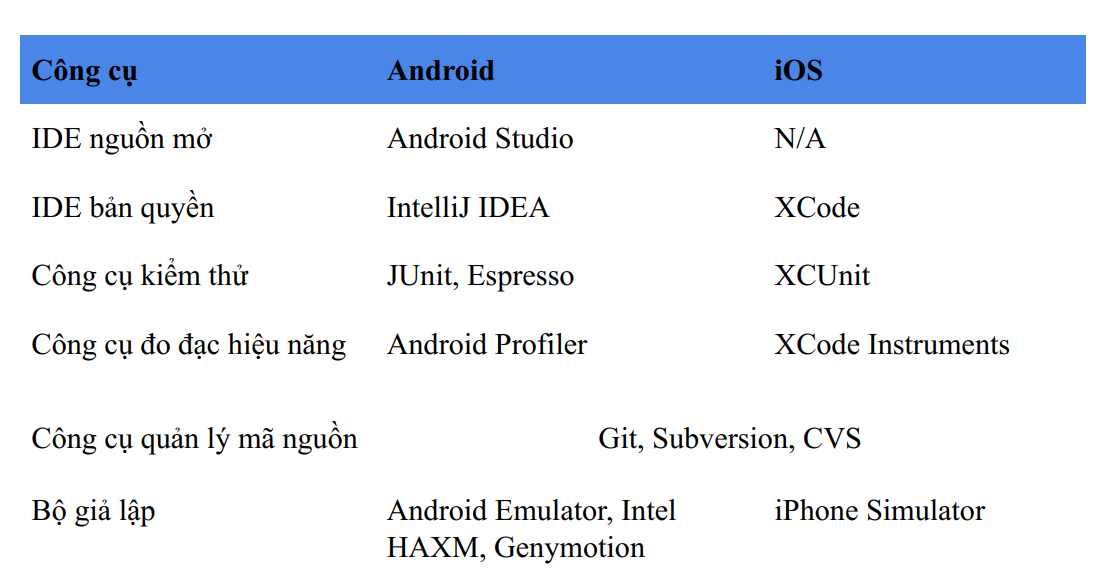
\includegraphics[width=0.95\textwidth]{images/cong-cu-android-ios.png}
    \caption{So sánh công cụ phát triển giữa Android và iOS \cite{ddiandroidios}}
    \label{fig:android_ios_tools}
  \end{figure}

  Hình~\ref{fig:android_ios_tools} thể hiện sự khác biệt giữa các công cụ được sử dụng trong hệ sinh thái Android và iOS. Việc lựa chọn công cụ phù hợp phụ thuộc vào hệ điều hành mục tiêu, ngôn ngữ lập trình và kinh nghiệm của lập trình viên.


% 2.2
\subsection{Các yếu tố quyết định khi lựa chọn đa nền tảng}
\renewcommand{\labelitemi}{--}    


  \subsubsection{Phân tích nhóm người dùng mục tiêu}
    
      Thị phần hệ điều hành đóng vai trò quan trọng trong việc xác định nền tảng ưu tiên.
      \setlength{\leftmargini}{1.5cm}
      \begin{itemize}
        \item iOS hiện chiếm 27\% thị trường toàn cầu, chủ yếu phổ biến tại Mỹ và Châu Âu.
        \item Android chiếm 73\%, đặc biệt thống trị tại Châu Á và Châu Phi (Ego-cms, 2021) ~\cite{egoMarketShare} .
      \end{itemize}
    \vspace{0.5em}

    
      Chiến lược tiếp cận người dùng cần phù hợp với đặc thù từng hệ điều hành.
      \setlength{\leftmargini}{1.5cm}
      \begin{itemize}
          \item Nếu đối tượng mục tiêu là người dùng cao cấp (iOS), nên ưu tiên framework hỗ trợ giao diện Cupertino như Flutter.
          \item Nếu nhắm tới thị trường đại chúng (Android), React Native là lựa chọn phù hợp nhờ khả năng tích hợp với Google Services.
      \end{itemize}
    \vspace{0.5em}

    
      Một ví dụ thực tế giúp minh họa rõ ràng cho lựa chọn nền tảng là Grab.
      \setlength{\leftmargini}{1.5cm}
      \begin{itemize}
          \item Grab (Flutter): Tập trung vào thị trường Đông Nam Á (đa số dùng Android) nhưng vẫn đảm bảo trải nghiệm mượt mà trên iOS.
      \end{itemize}

    \subsubsection{Mô hình "Rẻ – Nhanh – Tốt"}
    
      Nguyên tắc Iron Triangle cho rằng chỉ có thể đạt hai trong ba tiêu chí: rẻ, nhanh và tốt. Mỗi lựa chọn framework cần cân nhắc dựa trên ưu tiên này.
    \vspace{0.5em}

    \begin{figure}[H]
    \centering
    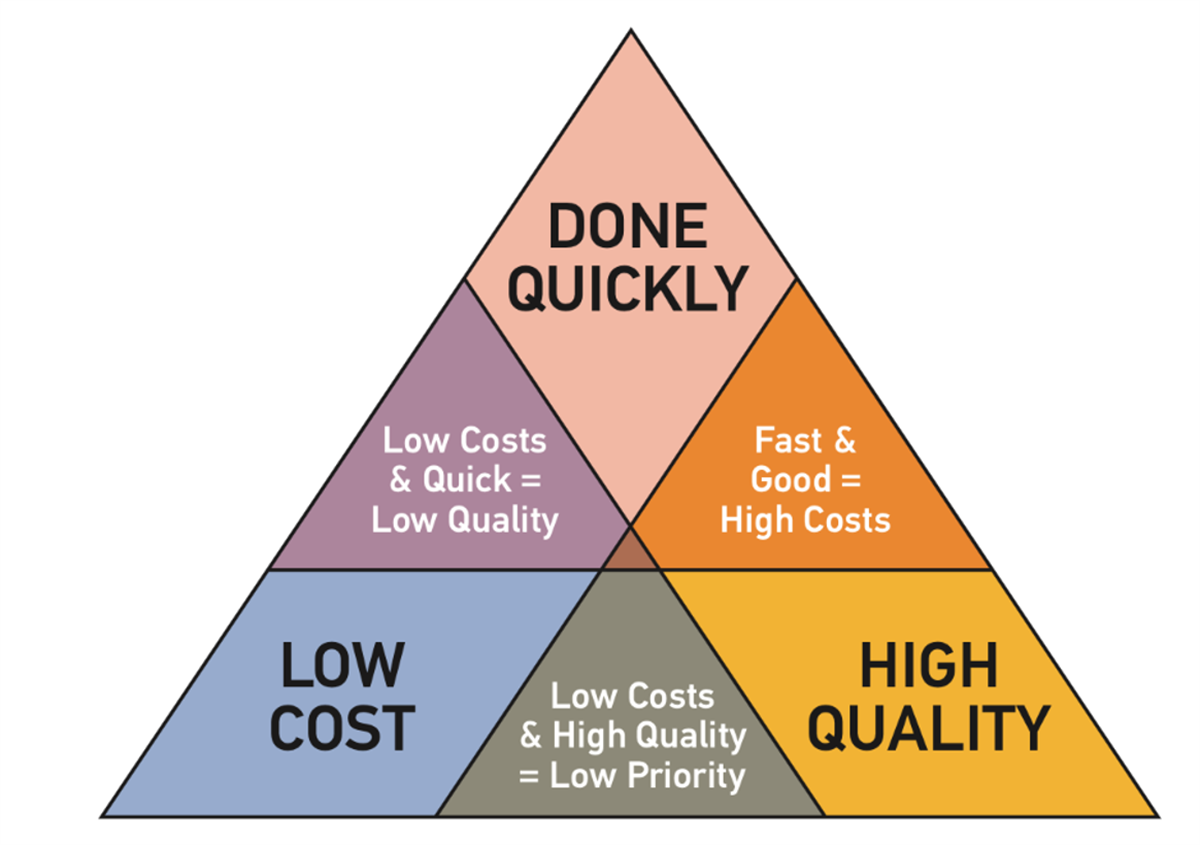
\includegraphics[width=0.45\textwidth]{images/iron_triangle.png}
    \caption{Mô hình Iron Triangle – Rẻ, Nhanh, Tốt – Chọn hai \cite{goodipidea2016}}
    \label{fig:android_ios_tools2}
  \end{figure}
    
      Tùy vào mục tiêu dự án, mỗi framework sẽ phù hợp với một chiến lược khác nhau.
      \setlength{\leftmargini}{1.5cm}
      \begin{itemize}
          \item React Native: Phù hợp cho dự án cần MVP (Minimum Viable Product) nhanh chóng, nhưng hiệu năng không cao.
          \item Flutter: Đòi hỏi đầu tư ban đầu để học Dart, nhưng mang lại hiệu năng cao và giao diện tùy biến tốt hơn.
      \end{itemize}
    

  \subsubsection{Khả năng tích hợp với hệ sinh thái hiện có}
      React Native tận dụng tốt hệ sinh thái JavaScript (Node.js, npm, Expo) và dễ tích hợp với ứng dụng web hiện tại.

      \vspace{0.5em}

      Flutter mặc dù độc lập hơn, nhưng vẫn có thể kết nối hiệu quả với Firebase hoặc Google Cloud thông qua plugin.

      \vspace{0.5em}
  
      Một ví dụ điển hình cho khả năng tích hợp là Shopify. Shopify sử dụng React Native để tích hợp ứng dụng mobile với nền tảng web sẵn có.

% 2.3
\subsection{Lịch sử phát triển của kiến trúc đa nền tảng}

\subsubsection{Thế hệ đầu tiên (2010–2015): WebView-based Frameworks}
Giai đoạn đầu tiên trong kiến trúc đa nền tảng là sự xuất hiện của các framework dựa trên WebView, điển hình là PhoneGap, Cordova, và Ionic. Các framework này hoạt động bằng cách đóng gói nội dung HTML/CSS/JavaScript trong WebView, tức bản chất ứng dụng chỉ là trình duyệt bên trong native shell.

\vspace{0.5em}

\indent Một ưu điểm lớn của các framework này là lập trình viên web có thể dễ dàng phát triển ứng dụng với chi phí phát triển và bảo trì thấp. Tuy nhiên, chúng có những hạn chế rõ ràng như hiệu năng thấp, không xử lý tốt các animation phức tạp, và giao diện thiếu tính bản địa hoá. Một ví dụ điển hình là ứng dụng Uber, ban đầu phát triển bằng Cordova nhưng phải chuyển sang native do hiện tượng lag khi hiển thị bản đồ.

\subsubsection{Thế hệ thứ hai (2015–2017): Hybrid Frameworks}

Sau WebView, thế hệ thứ hai ra đời với sự kết hợp giữa WebView và native components, gọi là Hybrid Frameworks, điển hình là Xamarin và NativeScript. Các framework này sử dụng cơ chế \textit{bridge} để kết nối JavaScript (hoặc C\#) với native APIs, cho phép sử dụng một số thành phần giao diện bản địa.

\vspace{0.5em}

\indent Hybrid frameworks mang lại hiệu năng cải thiện so với WebView và cho phép truy cập các native APIs như camera, GPS. Tuy nhiên, chúng vẫn có một số hạn chế như quá trình cấu hình phức tạp và dễ lỗi, và một số phần vẫn phải phụ thuộc vào WebView. Microsoft Outlook là ví dụ điển hình khi sử dụng Xamarin để phát triển ứng dụng đa nền tảng hiệu quả.

\subsubsection{Thế hệ hiện đại (2017–nay): Native-Reactive Frameworks}

 Từ năm 2017, kiến trúc đa nền tảng đã chuyển sang giai đoạn hiện đại với sự xuất hiện của các framework sử dụng native rendering, ví dụ như React Native và Flutter. Các framework này sử dụng cơ chế điều khiển native components thông qua bridge (React Native) hoặc tự vẽ giao diện mà không phụ thuộc vào hệ điều hành (Flutter).

\vspace{0.5em}

Nhờ cơ chế hiện đại, các framework này mang lại hiệu năng gần tương đương ứng dụng native và hỗ trợ đa nền tảng, từ mobile đến web và desktop. Một số bước đột phá quan trọng trong giai đoạn này gồm Flutter 2.0 (2020) mở rộng hỗ trợ nền tảng web và desktop, và React Native New Architecture (2022) sử dụng TurboModules và Fabric để tối ưu hiệu suất.

\vspace{0.5em}

\indent Ứng dụng Xianyu của Alibaba là ví dụ thành công khi sử dụng Flutter để phục vụ hơn 200 triệu người dùng, đạt hiệu năng tương đương ứng dụng native.
% 2.4
\subsection{Xu hướng tương lai của kiến trúc đa nền tảng}
\renewcommand{\labelitemi}{--}

\subsubsection{Tích hợp AI/ML trong phát triển}

Một trong những xu hướng quan trọng là việc tích hợp trí tuệ nhân tạo và học máy vào quy trình phát triển ứng dụng đa nền tảng. Thông qua công cụ như Google’s ML Kit, lập trình viên có thể tự động hóa các tác vụ như nhận diện hình ảnh và xử lý ngôn ngữ tự nhiên.

\vspace{0.5em}

AI không chỉ hỗ trợ tính năng thông minh, mà còn giúp tối ưu hiệu năng ứng dụng. Cụ thể, các hệ thống AI có thể phân tích mã nguồn để đề xuất cải thiện tốc độ khung hình (FPS) hoặc giảm tiêu thụ bộ nhớ RAM.

\vspace{0.5em}

Một ví dụ điển hình là Adobe XD, trong đó AI được sử dụng để tự động điều chỉnh giao diện người dùng dựa trên hành vi thực tế của người dùng.


\subsubsection{WebAssembly (Wasm) và Progressive Web Apps (PWA)}

WebAssembly đang nổi lên như một công nghệ quan trọng giúp ứng dụng chạy trên trình duyệt với hiệu năng gần tương đương ứng dụng native.  
Khả năng này giúp mở rộng phạm vi triển khai ứng dụng đa nền tảng trên môi trường web một cách hiệu quả.

\vspace{0.5em}

Cùng với đó, Progressive Web Apps (PWA) mang lại sự kết hợp giữa ứng dụng web và mobile app,  
hỗ trợ hoạt động offline và cho phép gửi thông báo đẩy đến người dùng như các ứng dụng native.

\vspace{0.5em}

Một ví dụ tiêu biểu là Starbucks, hãng đã triển khai PWA để tăng tốc độ tải trang và nâng cao trải nghiệm người dùng ngay cả khi không có kết nối mạng ổn định.


\subsubsection{Low-Code/No-Code Platforms}

Low-code và no-code platforms đang mở ra cơ hội mới cho cả những người không chuyên trong lĩnh vực lập trình. Với các nền tảng kéo–thả trực quan, người dùng có thể xây dựng ứng dụng đa nền tảng mà không cần viết bất kỳ dòng code nào.

\vspace{0.5em}

Lợi ích lớn nhất của mô hình này là rút ngắn thời gian phát triển và giảm thiểu chi phí đào tạo kỹ thuật, đặc biệt phù hợp với doanh nghiệp nhỏ hoặc bộ phận nội bộ cần triển khai nhanh giải pháp công nghệ.

\vspace{0.5em}

Chẳng hạn, Microsoft Power Apps đã giúp nhiều doanh nghiệp tạo ra ứng dụng quản lý nội bộ chỉ trong vài giờ làm việc.


% 2.5
\subsection{Case Study Chi Tiết}
\renewcommand{\labelitemi}{--}

\subsubsection{Airbnb và bài học từ React Native}

Airbnb đã từng áp dụng React Native với kỳ vọng tận dụng khả năng chia sẻ code giữa các nền tảng.  
Tuy nhiên, trong quá trình phát triển, họ gặp phải một số thách thức lớn. Cụ thể, nhóm phát triển gặp khó khăn trong việc tùy chỉnh giao diện người dùng phức tạp cho từng nền tảng, đặc biệt là khi phải đảm bảo trải nghiệm nhất quán và mượt mà. Ngoài ra, hiệu năng ứng dụng không đủ đáp ứng yêu cầu khi tích hợp tính năng đặt phòng theo thời gian thực, gây ảnh hưởng đến trải nghiệm người dùng cuối.

\vspace{0.5em}

Để giải quyết vấn đề này, Airbnb quyết định chuyển sang phát triển native cho các module quan trọng,  
đồng thời giữ lại React Native cho phần quản trị nội bộ nhằm tiết kiệm chi phí. Kết quả của chiến lược này là hiệu năng hệ thống được cải thiện 30\%,  
nhưng chi phí bảo trì cũng tăng lên khoảng 40\% do cần duy trì song song hai mã nguồn.

\subsubsection{Google Pay: Thành công với Flutter}

Google Pay là một trong những ví dụ điển hình cho việc ứng dụng thành công Flutter vào phát triển đa nền tảng. Chiến lược của nhóm phát triển là sử dụng một codebase duy nhất cho cả iOS, Android và web.

\vspace{0.5em}

Nhờ khả năng đồng bộ cao của Flutter, thời gian phát triển đã giảm tới 50\%, giúp nhóm ra mắt sản phẩm nhanh hơn mà vẫn đảm bảo chất lượng. Bên cạnh đó, hiệu năng ứng dụng cũng được đảm bảo, với tốc độ khung hình (FPS) ổn định ở mức 60 trên mọi thiết bị, tạo nên trải nghiệm người dùng mượt mà và đáng tin cậy.

\vspace{0.5em}

Tuy nhiên, nhóm cũng đối mặt với thách thức trong việc đào tạo đội ngũ kỹ thuật,  
đặc biệt là làm quen với ngôn ngữ Dart và cơ chế vẽ giao diện qua Skia Engine.

% 2.6
\subsection{So Sánh Chi Tiết React Native vs. Flutter}
\renewcommand{\labelitemi}{--}    

    Biểu đồ dưới đây so sánh mức độ quan tâm giữa hai framework di động phổ biến: \textbf{Flutter (xanh)} và \textbf{React Native (đỏ)} trong 12 tháng qua tại Hoa Kỳ, dựa trên dữ liệu tìm kiếm từ Google Trends.

    \begin{figure}[H]
        \centering
        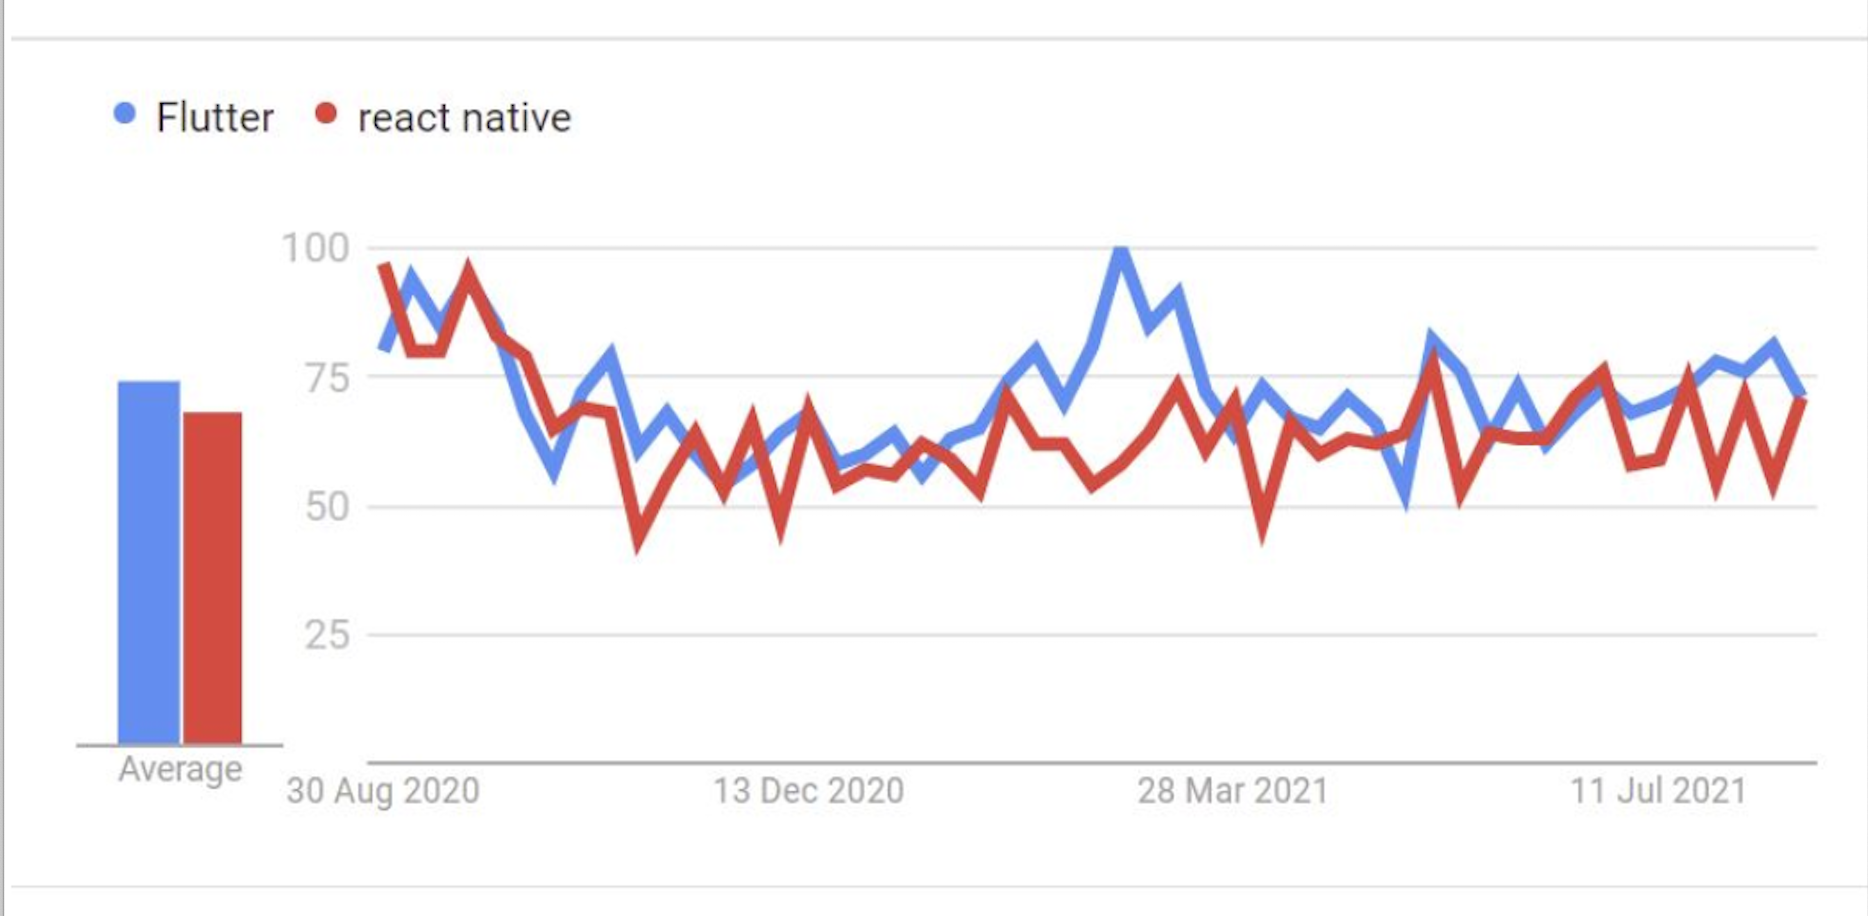
\includegraphics[width=0.9\textwidth]{images/reactNative_flutter.png}
        \caption{So sánh xu hướng tìm kiếm giữa Flutter và React Native \cite{goldenowlflutterreact}}
    \end{figure}

    Dưới đây là bảng so sánh một số khía cạnh chính giữa React Native và Flutter:

    \begin{table}[H]
        \centering
        \begin{tabular}{|l|p{3.5cm}|p{6cm}|}
            \hline
            \textbf{Tiêu chí} & \textbf{React Native} & \textbf{Flutter} \\
            \hline
            Ngôn ngữ lập trình & JavaScript (hoặc TypeScript) & Dart \\
            \hline
            Hiệu suất & Gần với native, phụ thuộc vào bridge & Cao hơn nhờ rendering engine riêng (Skia) \\
            \hline
            Giao diện người dùng & Dựa vào native components & Tùy chỉnh hoàn toàn, nhất quán mọi nền tảng \\
            \hline
            Cộng đồng & Lâu đời hơn, cộng đồng lớn & Đang phát triển nhanh chóng, được Google hỗ trợ mạnh \\
            \hline
            Tài liệu & Đầy đủ, nhiều ví dụ thực tiễn & Rõ ràng, cấu trúc tốt, phù hợp cho người mới bắt đầu \\
            \hline
        \end{tabular}
        \caption{So sánh các yếu tố giữa React Native và Flutter \cite{codetodeploy2025}}
    \end{table}

% 2.7
\subsection{Kết luận phần Cơ Sở Lý Thuyết}
\renewcommand{\labelitemi}{--}    
    
        Kiến trúc đa nền tảng đã phát triển qua nhiều giai đoạn, từ các giải pháp dựa trên WebView đến các framework hiện đại như React Native và Flutter. Mỗi công cụ có ưu nhược điểm riêng, phù hợp với từng loại dự án. Việc lựa chọn phụ thuộc vào sự cân nhắc giữa chi phí, thời gian, và chất lượng, cùng với định hướng dài hạn của doanh nghiệp. Xu hướng tương lai hứa hẹn sự tích hợp sâu rộng của AI, WebAssembly và low-code platforms, mở ra kỷ nguyên mới cho phát triển ứng dụng linh hoạt và hiệu quả.
\section{Phân Tích Các Framework}

  React Native và Flutter là hai framework đa nền tảng phổ biến, mỗi framework mang đến những ưu điểm và thách thức riêng. React Native, phát triển bởi Facebook, cho phép sử dụng JavaScript và tái sử dụng mã nguồn giữa các nền tảng iOS và Android, giúp tiết kiệm chi phí và thời gian phát triển. Với hệ sinh thái phong phú và cộng đồng lớn, React Native dễ dàng tích hợp với các công nghệ khác. Ngược lại, Flutter, do Google phát triển, sử dụng ngôn ngữ Dart và engine render riêng, giúp tối ưu hóa hiệu suất và tạo giao diện người dùng đẹp mắt, đồng thời mang lại hiệu quả cao trong việc phát triển ứng dụng yêu cầu đồ họa phức tạp. Tuy nhiên, Flutter còn thiếu sự phong phú của các plugin và thư viện như React Native. Việc lựa chọn giữa hai framework này phụ thuộc vào yêu cầu dự án, với React Native phù hợp cho các ứng dụng cần phát triển nhanh và dễ dàng tích hợp, còn Flutter thích hợp cho những ứng dụng yêu cầu hiệu suất và giao diện đặc biệt.

% 3.1
\subsection{React Native}
\renewcommand{\labelitemi}{--}    
\subsubsection{Kiến Trúc}

\begin{sloppypar}
React Native là một framework phát triển ứng dụng đa nền tảng do Meta (trước đây là Facebook) phát triển. Nó kết hợp giữa JavaScript và native code để xây dựng ứng dụng di động có giao diện mượt mà và khả năng mở rộng cao.
\end{sloppypar}

\vspace{0.5em}

\begin{sloppypar}
Kiến trúc của React Native bao gồm ba thành phần chính: \textbf{JavaScript VM}, \textbf{Bridge}, và \textbf{Native Modules}.
\end{sloppypar}

\vspace{0.5em}

\begin{figure}[H]
    \centering
    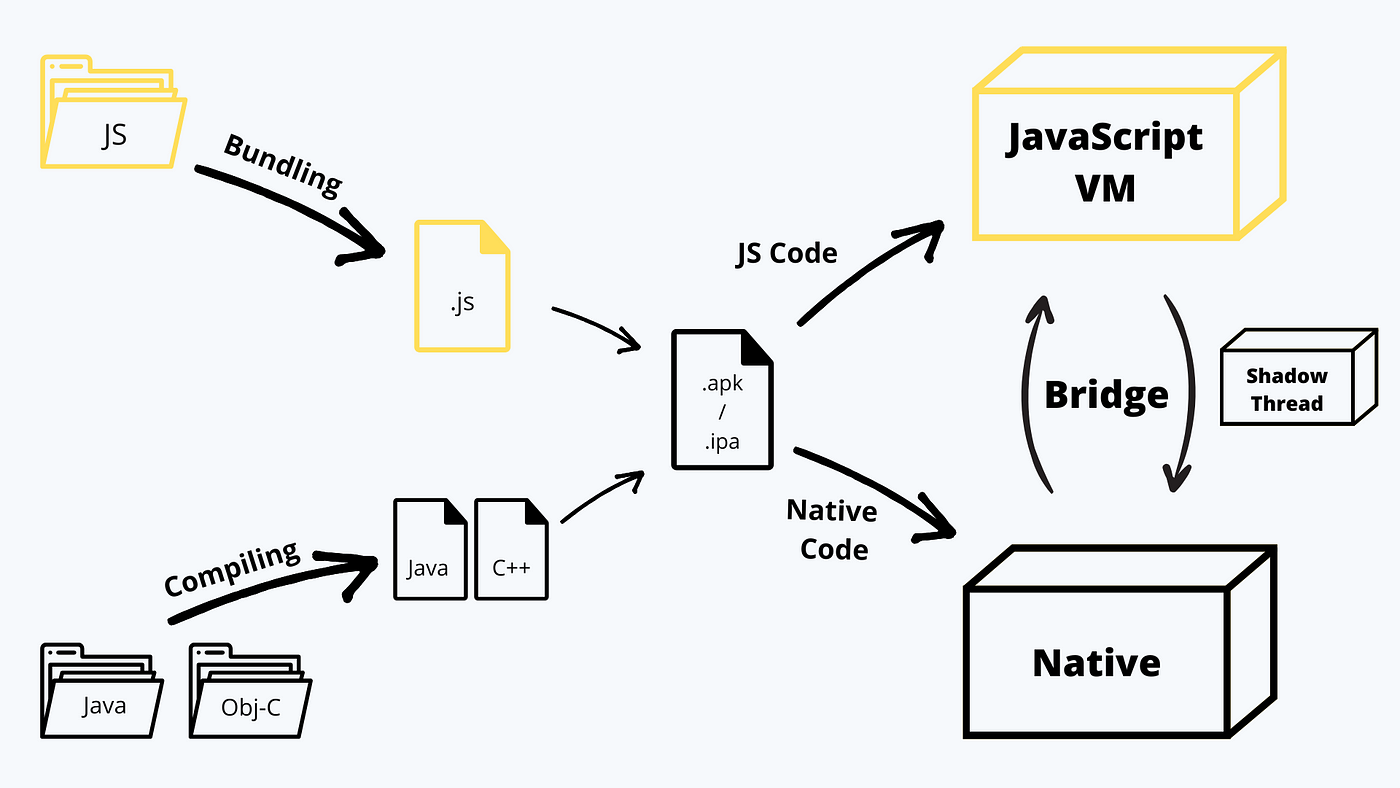
\includegraphics[width=0.95\textwidth]{images/react_native.png}
    \caption{Kiến trúc tổng quan của React Native~\cite{react-native-fabric}}
\end{figure}

\begin{sloppypar}
Trước tiên, JavaScript VM (Virtual Machine) là nơi thực thi logic nghiệp vụ của ứng dụng.  
Khi người dùng tương tác, các hàm JavaScript sẽ xử lý sự kiện, gọi API hoặc thao tác dữ liệu.  
Trên iOS, React Native sử dụng JavaScriptCore của WebKit; trên Android, Meta ưu tiên dùng Hermes – engine nhẹ giúp giảm thời gian khởi động 30\%.  
Ví dụ, Bloomberg đã sử dụng Hermes để tối ưu tốc độ cập nhật dữ liệu chứng khoán thời gian thực.
\end{sloppypar}

\vspace{0.5em}

\begin{sloppypar}
Tiếp theo, Native Modules là các thành phần được viết bằng ngôn ngữ nền tảng như Java/Kotlin hoặc Obj-C/Swift.  
Chúng cho phép ứng dụng truy cập các API hệ điều hành, ví dụ như GPS hoặc camera.  
Một ví dụ cụ thể là Walmart sử dụng Native Modules để tích hợp thanh toán NFC, đảm bảo hiệu suất và bảo mật cao.
\end{sloppypar}

\vspace{0.5em}

\begin{sloppypar}
Bridge đóng vai trò là cầu nối giữa JavaScript và native code.  
Khi JavaScript cần gọi chức năng nền tảng, Bridge sẽ truyền dữ liệu qua định dạng JSON – một quy trình tốn thời gian do phải serialize/\-deserialize.  
Theo Đại học Oslo (2022), việc giao tiếp này có thể gây trễ 5–15ms.  
Để khắc phục, Meta giới thiệu kiến trúc mới mang tên Fabric (2023), sử dụng JSI (JavaScript\- Interface) cho phép truy cập trực tiếp native code, giúp cải thiện tốc độ render đến 40\%.
\end{sloppypar}

\subsubsection{Ưu Điểm}
React Native mang lại nhiều lợi ích đáng kể, đặc biệt là khả năng tái sử dụng mã nguồn và tốc độ phát triển nhanh.

\vspace{0.5em}

Một trong những điểm mạnh lớn nhất là khả năng chia sẻ code giữa web và mobile. Ví dụ, Airbnb đã tái sử dụng đến 60\% codebase giữa hai nền tảng, tiết kiệm đáng kể thời gian phát triển. Thư viện \texttt{React Native Web} giúp chuyển đổi component React Native sang React DOM để chạy trên trình duyệt.

\vspace{0.5em}

Ngoài ra, hệ sinh thái npm khổng lồ (hơn 2.1 triệu package, 2023) giúp tăng tốc độ lập trình. Thư viện như \texttt{React Navigation} đơn giản hóa routing phức tạp, trong khi \texttt{React Native Maps} hỗ trợ hiển thị bản đồ chính xác.

\vspace{0.5em}

Cuối cùng, React Native cung cấp Live Reload và Hot Reload – hai công cụ giúp lập trình viên cập nhật UI ngay tức thì mà không mất trạng thái. Theo khảo sát của JetBrains (2022), tính năng này giúp rút ngắn thời gian debug đến 30\%.

\subsubsection{Nhược Điểm}

Dù có nhiều lợi ích, React Native vẫn tồn tại một số hạn chế nhất định, đặc biệt về hiệu năng và khả năng tùy biến.

\vspace{0.5em}

Do phụ thuộc vào Bridge, hiệu năng ứng dụng thấp hơn so với native. Ví dụ, render danh sách 1.000 phần tử trên React Native mất 320ms, trong khi native Android chỉ cần 210ms (Biorn-Hansen, 2021). Các ứng dụng yêu cầu đồ họa cao như game 3D hay video editor không phù hợp với React Native.

\vspace{0.5em}

Một vấn đề khác là phụ thuộc vào thư viện bên thứ ba. Khi nền tảng hệ điều hành thay đổi, các thư viện có thể không cập nhật kịp. Ví dụ, React Native Firebase gặp lỗi nghiêm trọng khi Android 13 thay đổi cơ chế cấp quyền, gây crash ứng dụng diện rộng.

\vspace{0.5em}

Cuối cùng, việc tùy chỉnh UI phức tạp như animation nâng cao hay tích hợp OpenGL đòi hỏi viết code native.  
Điều này làm tăng độ phức tạp và yêu cầu đội ngũ có kinh nghiệm phát triển native.

% 3.2
\subsection{Flutter}
\renewcommand{\labelitemi}{--}    
\subsubsection{Kiến Trúc}

Flutter là framework đa nền tảng do Google phát triển, sử dụng ngôn ngữ Dart và engine Skia để tự render giao diện người dùng, không phụ thuộc vào thành phần native.

\begin{figure}[H]
    \centering
    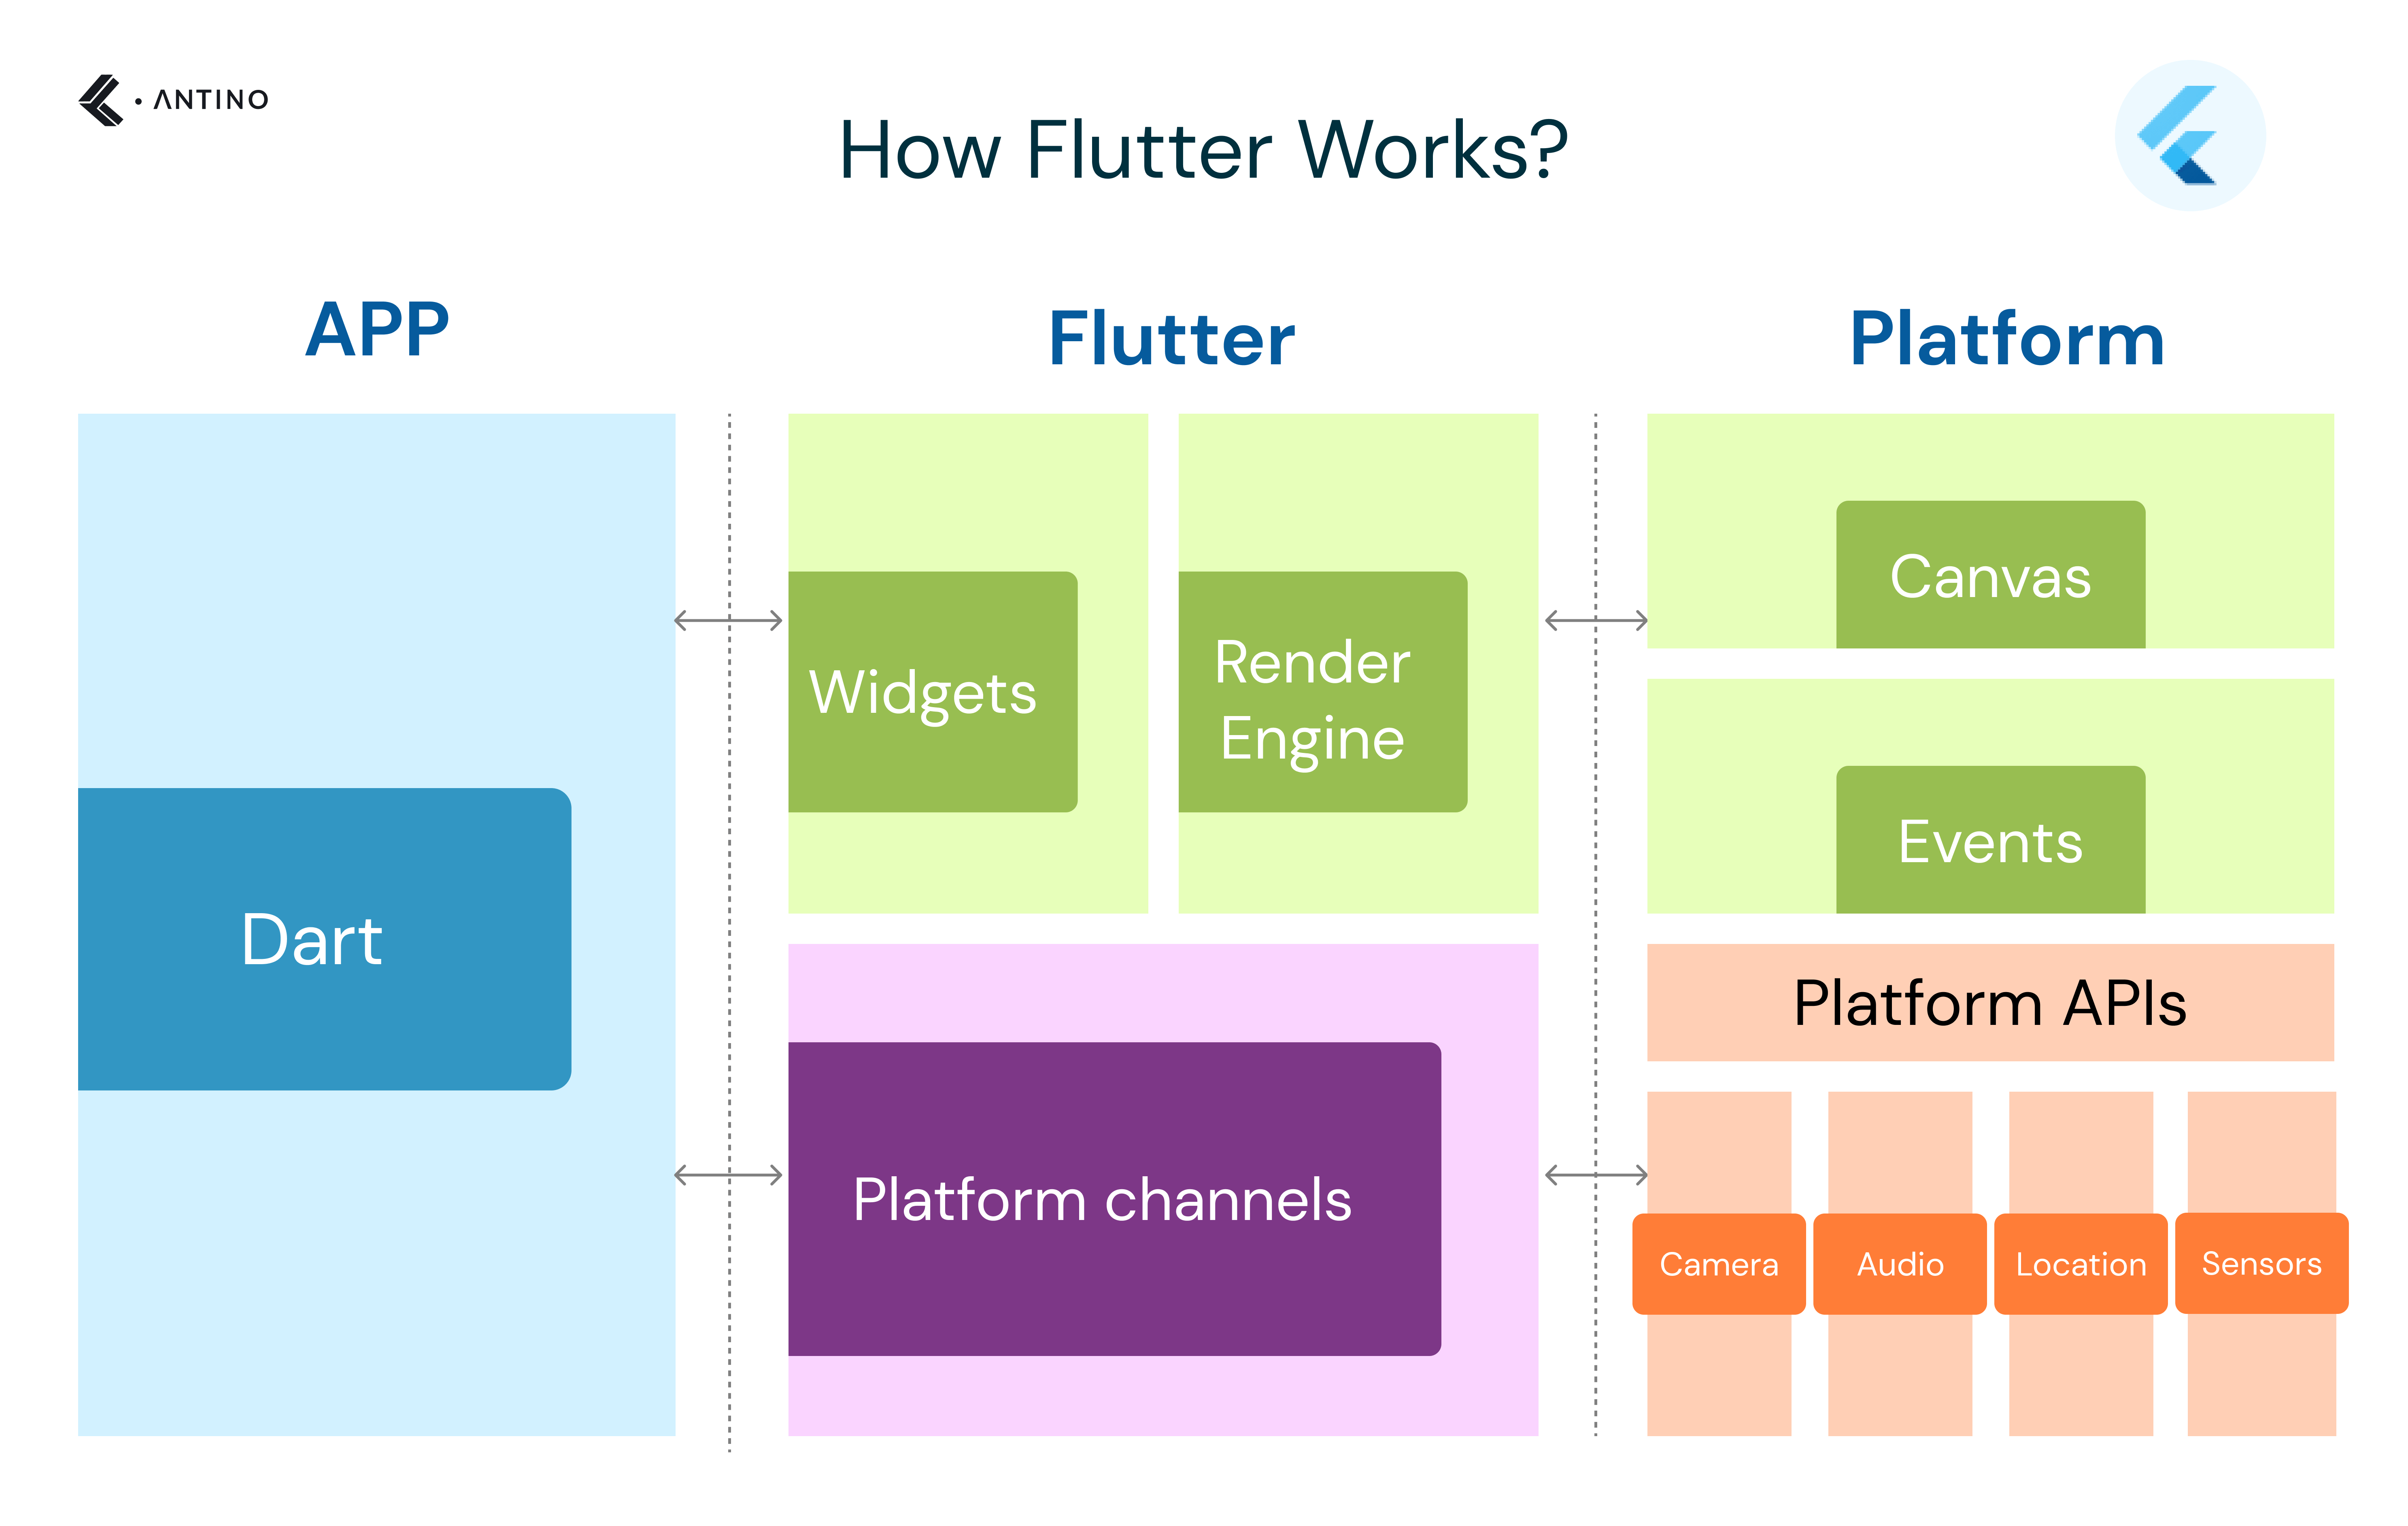
\includegraphics[width=0.75\textwidth]{images/flutter.png}
    \caption{Kiến trúc tổng quan của Flutter~\cite{flutter-impeller}}
\end{figure}

Dart là ngôn ngữ lập trình cốt lõi của Flutter, được thiết kế để kết hợp hiệu suất cao và tính linh hoạt. Dart hỗ trợ hai chế độ biên dịch: AOT (Ahead-of-Time) để tạo mã native tối ưu cho hiệu năng, và JIT (Just-in-Time) cho phép Hot Reload khi phát triển. Ví dụ, Alibaba đã dùng Dart để xử lý tới 50 triệu giao dịch/ngày, tận dụng khả năng xử lý bất đồng bộ hiệu quả với \texttt{Future}, \texttt{async/await}.

\vspace{0.5em}

Tiếp theo, engine Skia là thành phần chịu trách nhiệm vẽ toàn bộ UI lên một canvas duy nhất thay vì sử dụng native widgets. Điều này đảm bảo giao diện nhất quán trên mọi nền tảng. Chẳng hạn, nút \texttt{ElevatedButton} trong Flutter được render trực tiếp, cho phép tùy biến đến từng pixel. Ứng dụng như Starbucks hoặc eBay đã sử dụng Skia để đảm bảo tính thương hiệu trên iOS và Android đồng nhất.

\vspace{0.5em}

Flutter tổ chức UI theo mô hình widget – mọi thành phần đều là widget, kể cả layout và animation.  
Có hai loại chính:
\begin{itemize}
    \item \textbf{StatelessWidget}: không thay đổi trạng thái (ví dụ: văn bản tĩnh, biểu tượng).
    \item \textbf{StatefulWidget}: có thể thay đổi theo thời gian hoặc tương tác (ví dụ: checkbox, form).
\end{itemize}

Ngoài ra, Flutter hỗ trợ hai thư viện giao diện: \texttt{Material} (Google style) và \texttt{Cupertino} (iOS style), cho phép tạo trải nghiệm quen thuộc tùy theo nền tảng.

\vspace{0.5em}

Flutter giao tiếp với native thông qua \textbf{Platform Channels}, cho phép gọi các hàm nền tảng như GPS, camera hoặc Bluetooth.  
Ví dụ, khi ứng dụng cần truy cập cảm biến gia tốc, Flutter sẽ gửi message qua channel và native sẽ trả về dữ liệu tương ứng.

\subsubsection{Ưu Điểm}

Flutter nổi bật nhờ hiệu năng cao và khả năng tùy chỉnh mạnh:

\vspace{0.5em}

Thứ nhất, Flutter có hiệu năng gần như native nhờ sử dụng AOT compilation.  
Các ứng dụng như Google Pay đạt 60 FPS ngay cả trên thiết bị cấu hình thấp, với độ trễ phản hồi giao dịch dưới 100ms.

\vspace{0.5em}

Thứ hai, tính năng \textbf{Hot Reload} cho phép lập trình viên cập nhật giao diện tức thì mà không mất trạng thái ứng dụng.  
Theo báo cáo từ BMW, tính năng này đã giúp nhóm thiết kế UI giảm tới 50\% thời gian phát triển.

\vspace{0.5em}

Thứ ba, Flutter hỗ trợ đa nền tảng từ một codebase duy nhất, bao gồm Android, iOS, web, Windows, macOS và Linux. Ví dụ, ứng dụng Reflectly đạt 95\% tái sử dụng mã nguồn, giúp giảm 70\% chi phí bảo trì so với phát triển riêng lẻ từng nền tảng.

\subsubsection{Nhược Điểm}

Mặc dù có nhiều ưu điểm, Flutter vẫn còn một số hạn chế kỹ thuật đáng lưu ý:

\vspace{0.5em}

Đầu tiên, kích thước ứng dụng Flutter tương đối lớn.  
Một ứng dụng Flutter trống có thể lên đến 20MB, do nhúng sẵn Dart runtime và Skia engine – lớn hơn nhiều so với React Native (khoảng 4MB).  
Điều này ảnh hưởng đến người dùng ở khu vực có tốc độ Internet chậm.

\vspace{0.5em}

Tiếp theo, lập trình viên phải học ngôn ngữ Dart – vốn chưa phổ biến như JavaScript. Cú pháp Dart tương đối mới với nhiều người, đặc biệt trong xử lý bất đồng bộ sử dụng \texttt{Future}, \texttt{Stream} thay vì \texttt{Promise} như trong JS.

\vspace{0.5em}

Cuối cùng, hệ sinh thái thư viện của Flutter nhỏ hơn React Native. Tính đến 2023, Flutter có khoảng 25.000 package trên pub.dev, so với hơn 50.000 package của React Native trên npm. Điều này khiến việc tìm thư viện phù hợp đôi khi gặp hạn chế, đặc biệt với các chức năng phức tạp hoặc mới xuất hiện.

% 3.3
\subsection{So sánh React Native và Flutter}
\renewcommand{\labelitemi}{--}

\subsubsection{Hiệu năng khi cuộn (Scrolling)}

  Theo biểu đồ Figure~\ref{fig:scrolling}, Flutter duy trì tốc độ khung hình ổn định gần 60 FPS trong khi React Native có hiện tượng drop mạnh xuống dưới 30 FPS do độ trễ từ bridge giữa UI thread và JavaScript thread. Điều này cho thấy Flutter có hiệu năng cuộn mượt mà hơn, thích hợp với các ứng dụng có nhiều tương tác như game hoặc trình chỉnh sửa ảnh.

\begin{figure}[H]
    \centering
    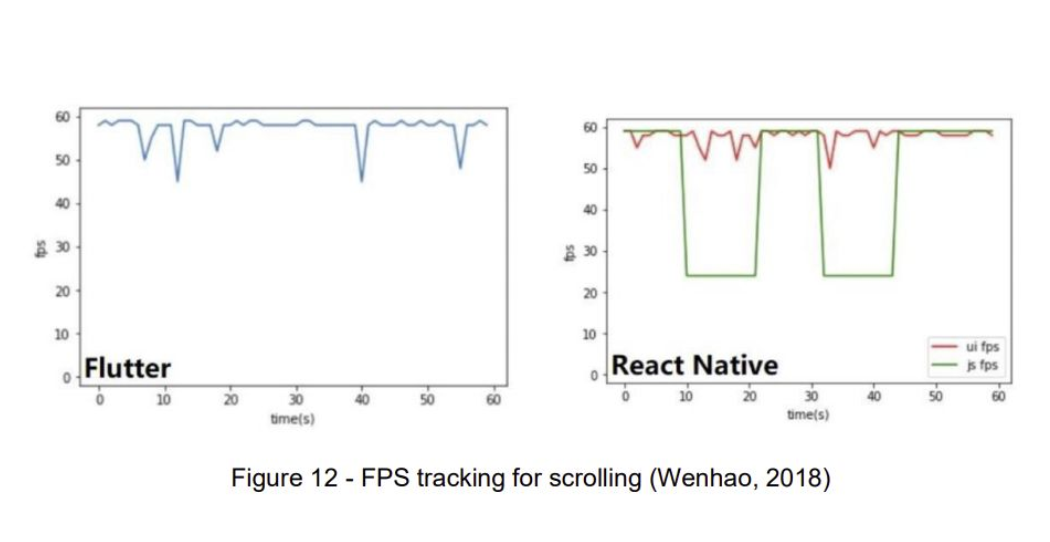
\includegraphics[width=0.8\linewidth]{images/scrolling.png}
    \caption{FPS khi cuộn của Flutter và React Native (Wenhao, 2018)}
    \label{fig:scrolling}
\end{figure}

\subsubsection{Ghi dữ liệu (Write Performance)}

  Biểu đồ Figure~\ref{fig:write} cho thấy thời gian ghi đơn lẻ và trung bình của React Native thấp hơn Flutter, phản ánh hiệu suất tốt hơn ở tác vụ ghi nhẹ. Tuy nhiên, chênh lệch không quá lớn và có thể không đáng kể trong hầu hết ứng dụng thực tế.

\begin{figure}[H]
    \centering
    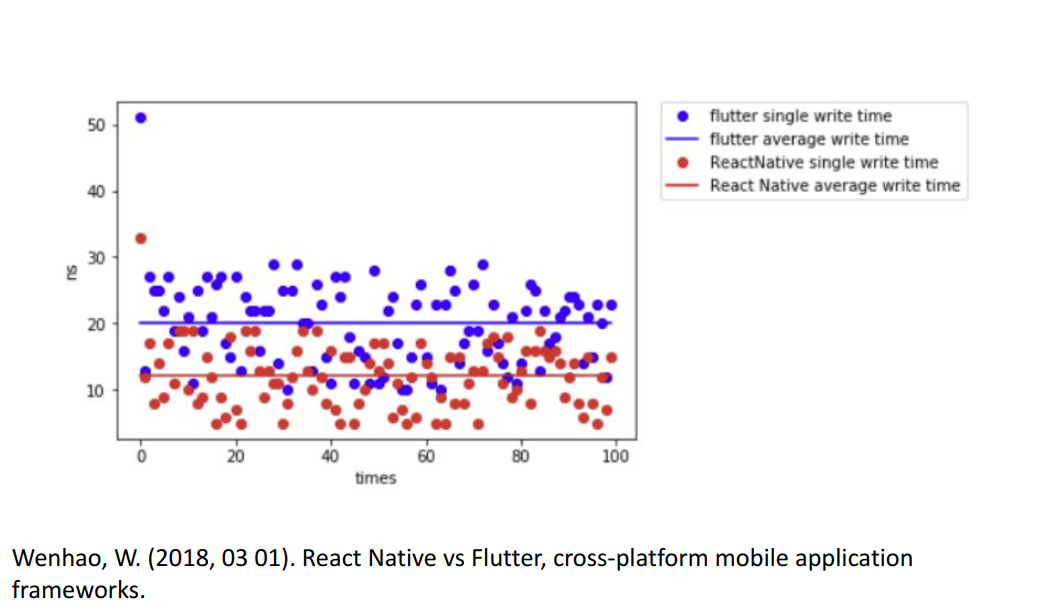
\includegraphics[width=0.8\linewidth]{images/read_write.png}
    \caption{Hiệu suất ghi dữ liệu của Flutter và React Native (Wenhao, 2018)}
    \label{fig:write}
\end{figure}

\subsubsection{Hiệu năng tổng thể theo nghiên cứu mới nhất}

  Theo Biorn-Hansen (2021), React Native và Flutter có điểm tổng thể thấp hơn Native, MAML/MD\textsuperscript{2} và NativeScript về hiệu năng cầu nối (bridge performance). Flutter đạt tổng điểm 15, thấp hơn React Native (16), chủ yếu do sử dụng nhiều RAM tính toán hơn. Tuy nhiên, Flutter vẫn là lựa chọn đáng cân nhắc nếu hiệu năng hình ảnh (UI performance) là yếu tố ưu tiên.

\begin{figure}[H]
    \centering
    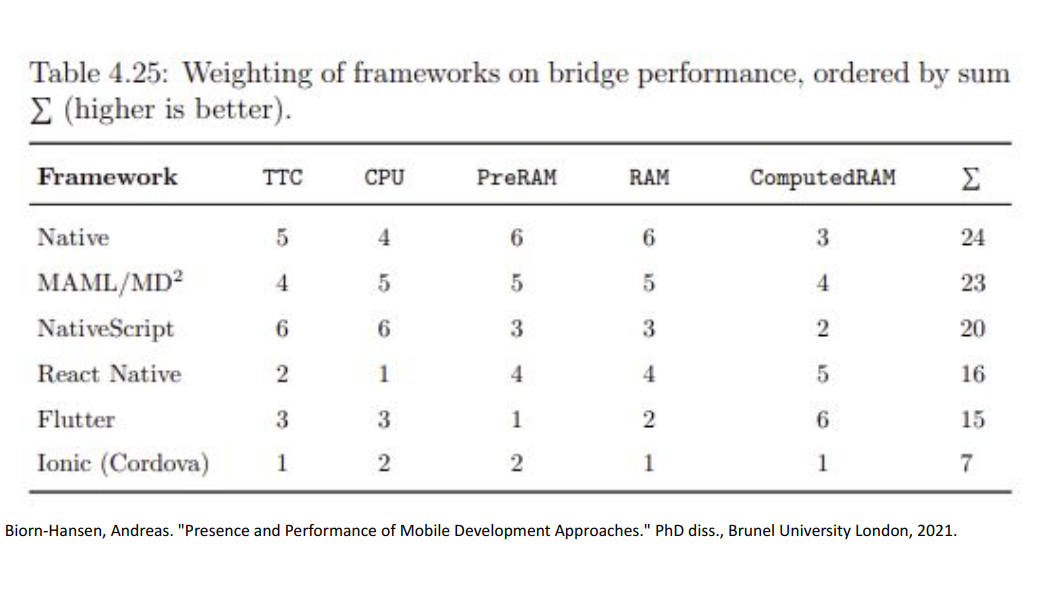
\includegraphics[width=0.7\linewidth]{images/performance.png}
    \caption{Đánh giá hiệu năng framework theo Biorn-Hansen (2021)}
    \label{fig:overall}
\end{figure}

\subsubsection{Ngôn ngữ lập trình}

  React Native sử dụng JavaScript – một ngôn ngữ phổ biến, dễ học, hỗ trợ từ hệ sinh thái Node.js và thư viện lớn. Trong khi đó, Flutter dùng Dart – một ngôn ngữ được Google phát triển với ưu điểm về type safety và khả năng biên dịch AOT, giúp giảm lỗi runtime nhưng đòi hỏi thời gian làm quen.

\subsubsection{Phát triển đa nền tảng}

  React Native chủ yếu nhắm đến iOS và Android, tuy có hỗ trợ web nhưng chưa ổn định. Ngược lại, Flutter hỗ trợ 6 nền tảng gồm mobile, web và desktop (Windows, macOS, Linux), phù hợp với ứng dụng cần độ bao phủ rộng và giao diện đồng nhất.

\subsubsection{Cộng đồng và tài nguyên}

  React Native sở hữu cộng đồng lớn với hơn 2 triệu developer, tài nguyên phong phú trên Stack Overflow, GitHub và blog kỹ thuật. Flutter tuy mới hơn nhưng đang tăng trưởng nhanh, đặc biệt ở thị trường châu Á, được Google đầu tư mạnh về tài liệu và hỗ trợ chính thức.

% 3.4
\subsection{Case Study}
\renewcommand{\labelitemi}{--}    
\subsubsection{React Native: Instagram}

  Instagram đã tích hợp React Native vào ứng dụng native hiện có nhằm tăng tốc độ phát triển các tính năng như \textit{Stories} và giao diện máy ảnh (\textit{Camera UI}). Một trong những thách thức chính là đảm bảo hiệu năng ổn định trên các thiết bị cũ như iPhone 6s. Đội ngũ phát triển đã áp dụng kỹ thuật \textit{lazy loading} để tải component khi cần thiết và tối ưu cầu nối (\textit{bridge}) bằng cách giảm thiểu số lần tương tác giữa JavaScript và native thread. Kết quả, họ tái sử dụng được khoảng 85\% mã nguồn giữa hai nền tảng iOS và Android, đồng thời rút ngắn 30\% thời gian phát triển tính năng.

\subsubsection{Flutter: Google Ads}

  Ứng dụng Google Ads được xây dựng bằng Flutter nhằm hỗ trợ quản lý quảng cáo trên nhiều nền tảng. Ứng dụng này xử lý trung bình 5 triệu request mỗi ngày từ 16 quốc gia, với yêu cầu độ trễ phản hồi không vượt quá 200ms. Nhóm phát triển đã tận dụng \textit{Dart isolates} để thực hiện các tác vụ tính toán nặng ở luồng phụ, kết hợp với Firebase để đồng bộ dữ liệu thời gian thực (\textit{real-time}). Kết quả là thời gian tải dữ liệu giảm 40\%, đồng thời giao diện người dùng duy trì tốc độ khung hình 60 FPS trên tất cả thiết bị, bao gồm cả thiết bị cấu hình thấp.

% 3.5
\subsection{Kết Luận}
\renewcommand{\labelitemi}{--}    

  Cả React Native và Flutter đều là những framework hàng đầu cho phát triển ứng dụng đa nền tảng. Tuy nhiên, mỗi công nghệ lại phù hợp với những mục tiêu và điều kiện cụ thể trong quá trình phát triển.
  
  \setlength{\leftmargini}{1.5cm}
  \begin{itemize}
    \item Đối với các startup mong muốn đưa sản phẩm ra thị trường nhanh chóng, React Native là lựa chọn lý tưởng nhờ khả năng tái sử dụng mã JavaScript và cộng đồng phát triển rộng lớn.
    \item Trong khi đó, Flutter thể hiện ưu thế vượt trội ở những dự án yêu cầu hiệu năng cao và giao diện người dùng tuỳ chỉnh phức tạp nhờ engine đồ hoạ tích hợp và khả năng biên dịch trực tiếp sang mã máy.
  \end{itemize}
\vspace{0.5em}


  Trong tương lai, cả hai framework đều đang theo đuổi các hướng phát triển mới nhằm mở rộng phạm vi ứng dụng.

  \setlength{\leftmargini}{1.5cm}
  \begin{itemize}
    \item Flutter được kỳ vọng sẽ mở rộng sang các hệ thống nhúng như thiết bị IoT hoặc ô tô thông minh, đặc biệt thông qua dự án Hummingbird.
    \item Ngược lại, React Native đang tập trung vào cải thiện hiệu năng lõi bằng các sáng kiến như Fabric và TurboModules, giúp tối ưu giao tiếp giữa native và JavaScript.
  \end{itemize}
\vspace{0.5em}


  Việc lựa chọn framework phù hợp nên dựa trên các tiêu chí rõ ràng về kỹ thuật và nguồn lực.

  \setlength{\leftmargini}{1.5cm}
  \begin{itemize}
    \item Trước khi quyết định, nhóm phát triển nên đánh giá yêu cầu về giao diện, hiệu năng, cũng như kỹ năng sẵn có trong đội ngũ.
    \item Bên cạnh đó, việc xây dựng nguyên mẫu (\textit{prototype}) bằng cả hai công nghệ để kiểm thử hiệu suất thực tế là cách tiếp cận thực tiễn và hiệu quả.
  \end{itemize}

\section{Phân tích chi tiết các kiến trúc phần mềm}

% 
\subsection{Kiến trúc phần mềm ba tầng (Three-tier architecture)}
\renewcommand{\labelitemi}{--}    
    \begin{flushleft}
        \hspace*{0.8cm}Đây là một mô hình tổ chức phần mềm phổ biến, đặc biệt phù hợp với các hệ thống lớn, có khả năng mở rộng và bảo trì lâu dài. Mô hình này phân chia rõ ràng trách nhiệm của từng tầng, từ việc hiển thị, xử lý logic cho đến lưu trữ dữ liệu. Việc áp dụng kiến trúc ba tầng giúp ứng dụng dễ bảo trì, linh hoạt trong mở rộng và tăng khả năng tái sử dụng mã nguồn.
    \end{flushleft}

    \begin{flushleft}
      \hspace*{0.8cm}Kiến trúc ba tầng có thể áp dụng cho nhiều loại ứng dụng khác nhau: từ ứng dụng đơn giản đến phức tạp, từ ứng dụng độc lập đến ứng dụng kết nối mạng. Việc tách biệt ba tầng không chỉ làm cho mã nguồn trở nên rõ ràng hơn mà còn cho phép các nhóm phát triển làm việc độc lập trên từng tầng.
    \end{flushleft}

    \begin{flushleft}
      \hspace*{0.8cm}Tầng trình diễn (Presentation Layer), đây là tầng giao tiếp với người dùng. Chức năng chính của tầng này bao gồm:
      \setlength{\leftmargini}{1.5cm}
      \begin{itemize}
          \item Hiển thị dữ liệu từ tầng nghiệp vụ theo giao diện trực quan.
          \item Nhận lệnh từ người dùng (qua các nút bấm, form, tương tác giao diện).
          \item Không xử lý logic nghiệp vụ, nhờ vậy giao diện có thể dễ dàng tái sử dụng, thay đổi hoặc cập nhật mà không ảnh hưởng đến các tầng khác.
          \item[]$\Rightarrow$ Một lợi ích lớn là khả năng “lắp ghép” lại với các tầng nghiệp vụ khác nhau – giúp cùng một giao diện có thể sử dụng cho nhiều phiên bản khác nhau của hệ thống.
      \end{itemize}
    \end{flushleft}

    \begin{flushleft}
      \hspace*{0.8cm}Tầng nghiệp vụ (Business Logic Layer), tầng này giữ vai trò trung tâm trong hệ thống. Nó thực hiện:
      \setlength{\leftmargini}{1.5cm}
      \begin{itemize}
          \item Chuẩn bị dữ liệu đầu vào để gửi đến tầng dữ liệu.
          \item Chuyển đổi, xử lý dữ liệu nhận về để trả lại cho tầng trình diễn.
          \item Xử lý các lỗi logic hoặc lỗi phản hồi từ tầng dữ liệu.
          \item Áp dụng các quy tắc nghiệp vụ, như kiểm tra hợp lệ, xử lý quy trình.
          \item[]$\Rightarrow$ Tầng này giúp cô lập các xử lý phức tạp khỏi giao diện và dữ liệu, đảm bảo khả năng kiểm thử và bảo trì cao.
      \end{itemize}
    \end{flushleft}

    \begin{flushleft}
      \hspace*{0.8cm}Tầng dữ liệu (Data Layer), là nơi lưu trữ các thông tin quan trọng nhất của ứng dụng:
      \setlength{\leftmargini}{1.5cm}
      \begin{itemize}
          \item Lưu trữ cơ sở dữ liệu (SQL, NoSQL…).
          \item Thực hiện các truy vấn để đảm bảo hiệu năng và độ chính xác cao.
          \item Có thể tích hợp với cơ sở dữ liệu từ xa (server), hệ thống lưu trữ đám mây hoặc tệp cục bộ.
          \item[]$\Rightarrow$ Việc tối ưu tầng dữ liệu giúp cải thiện đáng kể hiệu năng của toàn hệ thống, đặc biệt là trong các ứng dụng có lượng dữ liệu lớn.
      \end{itemize}
    \end{flushleft}

    \begin{flushleft}
      \hspace*{0.8cm}$\Rightarrow$ Kiến trúc ba tầng mang lại lợi ích lớn về mặt tổ chức mã nguồn, bảo trì, kiểm thử và phát triển theo nhóm. Mỗi tầng có trách nhiệm riêng, từ đó giúp ứng dụng dễ mở rộng và thích ứng với thay đổi trong tương lai.
    \end{flushleft}

% 4.2
\subsection{Kiến trúc MVC (Model – View – Controller)}
\renewcommand{\labelitemi}{--}    
    \begin{flushleft}
        \hspace*{0.8cm}MVC (Model – View – Controller) là một mẫu kiến trúc phần mềm cổ điển, phổ biến trong phát triển ứng dụng, đặc biệt là trên nền tảng iOS. Mục tiêu chính của kiến trúc MVC là tách biệt rõ ràng giữa dữ liệu, giao diện và điều khiển xử lý, từ đó giúp ứng dụng dễ bảo trì, mở rộng và nâng cao trải nghiệm người dùng.
    \end{flushleft}

    \begin{flushleft}
      \hspace*{0.8cm}Mô hình này được hình dung như một sơ đồ ba thành phần, mỗi thành phần đảm nhận một vai trò cụ thể:
      \setlength{\leftmargini}{1.5cm}
      \begin{itemize}
          \item Model: Dữ liệu và logic xử lý dữ liệu.
          \item View: Giao diện hiển thị cho người dùng.
          \item Controller: Bộ điều phối, tiếp nhận hành động từ người dùng và điều khiển luồng xử lý.
          \item[]$\Rightarrow$ Ba thành phần hoạt động tách biệt nhưng liên kết chặt chẽ, đảm bảo ứng dụng vận hành trơn tru và dễ dàng điều chỉnh một phần mà không ảnh hưởng đến phần còn lại.
      \end{itemize}
    \end{flushleft}

    \begin{flushleft}
      \hspace*{0.8cm}Model – Mô hình dữ liệu:
      \setlength{\leftmargini}{1.5cm}
      \begin{itemize}
          \item Định danh những gì cần trả về cho người dùng.
          \item Đây là nơi chứa dữ liệu thô, các quy tắc nghiệp vụ và các thao tác xử lý dữ liệu.
          \item Ví dụ: trong một ứng dụng bán hàng, Model chứa thông tin sản phẩm, đơn hàng, người dùng...
      \end{itemize}
    \end{flushleft}

    \begin{flushleft}
      \hspace*{0.8cm}Controller – Bộ điều khiển:
      \setlength{\leftmargini}{1.5cm}
      \begin{itemize}
          \item Tiếp nhận các yêu cầu từ người dùng (qua View).
          \item Thực hiện các truy vấn tài nguyên, gọi các phương thức xử lý trong Model.
          \item Là “bộ não” điều phối mọi hoạt động trong ứng dụng.
      \end{itemize}
    \end{flushleft}

    \begin{flushleft}
      \hspace*{0.8cm}View – Giao diện người dùng:
      \setlength{\leftmargini}{1.5cm}
      \begin{itemize}
          \item Hiển thị dữ liệu dưới dạng dễ hiểu, thân thiện với người dùng.
          \item View không xử lý logic nghiệp vụ, mà chỉ phản hồi lại theo những gì Controller và Model cung cấp.
          \item View sẽ cập nhật nội dung mỗi khi Model thay đổi.
      \end{itemize}
    \end{flushleft}

    \begin{flushleft}
      \hspace*{0.8cm}MVC giúp tách biệt rõ ràng chức năng, dễ dàng phát triển, kiểm thử và bảo trì. Đồng thời cho phép nhiều lập trình viên làm việc song song: người thiết kế giao diện làm View, lập trình viên backend làm Model, còn Controller kết nối hai phần này. Ngoài ra, nó còn có tính tái sử dụng mã nguồn tốt khi một Model có thể được dùng cho nhiều View khác nhau.
    \end{flushleft}

    \begin{flushleft}
      \hspace*{0.8cm}$\Rightarrow$ Mẫu kiến trúc MVC là một giải pháp hiệu quả giúp tổ chức ứng dụng một cách khoa học và linh hoạt. Việc phân chia ứng dụng thành ba thành phần rõ ràng giúp giảm độ phức tạp khi mở rộng, dễ bảo trì, đồng thời nâng cao hiệu quả làm việc nhóm trong quá trình phát triển ứng dụng. Với iOS, MVC vẫn là lựa chọn được ưa chuộng và hỗ trợ tốt trong môi trường phát triển Xcode và Swift.
    \end{flushleft}

% 4.3
\subsection{Kiến trúc MVVM (Model - View - ViewModel)}
\renewcommand{\labelitemi}{--}    
    \begin{flushleft}
        \hspace*{0.8cm}Kiến trúc MVVM (Model – View – ViewModel) là một trong những mẫu thiết kế hiện đại, được áp dụng phổ biến trong phát triển ứng dụng Android (đặc biệt là với sự hỗ trợ từ Jetpack và Kotlin). MVVM ra đời nhằm tối ưu quá trình phát triển ứng dụng bằng cách tách biệt logic hiển thị và logic xử lý, đồng thời tăng tính tự động hóa trong việc cập nhật dữ liệu nhờ cơ chế Data Binding.
    \end{flushleft}

    \begin{flushleft}
      \hspace*{0.8cm}MVVM có cấu trúc gần giống với MVC, nhưng thay vì để Controller điều khiển toàn bộ luồng xử lý, MVVM đưa vào một tầng trung gian là ViewModel – chịu trách nhiệm “kết nối thông minh” giữa dữ liệu (Model) và giao diện (View):
      \setlength{\leftmargini}{1.5cm}
      \begin{itemize}
          \item Tương tự như MVC, View hiển thị dữ liệu, Model chứa dữ liệu và logic xử lý.
          \item Tuy nhiên, Controller được thay thế bằng ViewModel, giúp giảm bớt sự ràng buộc giữa View và Model.
      \end{itemize}
    \end{flushleft}

    \begin{flushleft}
      \hspace*{0.8cm}Model – Dữ liệu và logic xử lý:
      \setlength{\leftmargini}{1.5cm}
      \begin{itemize}
          \item Là nơi lưu trữ các dữ liệu chính của ứng dụng (như thông tin người dùng, sản phẩm...).
          \item Xử lý các nghiệp vụ như tính toán, truy xuất dữ liệu từ cơ sở dữ liệu hoặc API.
          \item Model không trực tiếp liên hệ với View, mà thông qua ViewModel.
      \end{itemize}
    \end{flushleft}

    \begin{flushleft}
      \hspace*{0.8cm}View – Giao diện hiển thị:
      \setlength{\leftmargini}{1.5cm}
      \begin{itemize}
          \item Là phần người dùng tương tác trực tiếp (giao diện ứng dụng).
          \item View trong MVVM không xử lý logic nghiệp vụ mà chỉ phản ánh lại các dữ liệu từ ViewModel.
          \item Nhờ vào Data Binding, View có thể tự động cập nhật khi dữ liệu trong ViewModel thay đổi – giúp giảm mã lặp và tăng hiệu suất phát triển.
      \end{itemize}
    \end{flushleft}

    \begin{flushleft}
      \hspace*{0.8cm}ViewModel – Cầu nối thông minh:
      \setlength{\leftmargini}{1.5cm}
      \begin{itemize}
          \item Chứa các Model và chuẩn bị dữ liệu để hiển thị cho View.
          \item Tạo ra các LiveData hoặc Observable để View có thể theo dõi và tự động cập nhật giao diện khi dữ liệu thay đổi.
          \item Đồng thời, ViewModel cũng xử lý việc truyền dữ liệu từ View sang Model, giúp cập nhật ngược lại khi người dùng nhập liệu hoặc thực hiện thao tác.
      \end{itemize}
    \end{flushleft}

    \begin{flushleft}
      \hspace*{0.8cm}Một điểm mạnh nổi bật của MVVM là cơ chế Data Binding – liên kết dữ liệu hai chiều:
      \setlength{\leftmargini}{1.5cm}
      \begin{itemize}
          \item Khi một đối tượng thuộc nhóm View (như EditText) thay đổi, dữ liệu tương ứng trong ViewModel (hoặc Model) cũng tự động cập nhật.
          \item Ngược lại, khi ViewModel thay đổi giá trị, View cũng cập nhật lại ngay lập tức.
          \item[]$\Rightarrow$ Điều này giúp hạn chế lỗi khi cập nhật giao diện và rút ngắn thời gian phát triển, đặc biệt là trong các ứng dụng có nhiều thao tác tương tác dữ liệu.
      \end{itemize}
    \end{flushleft}

    \begin{flushleft}
      \hspace*{0.8cm}$\Rightarrow$ MVVM là một mô hình kiến trúc mạnh mẽ, phù hợp với các ứng dụng hiện đại cần cập nhật giao diện linh hoạt, liên tục. Với sự hỗ trợ từ Data Binding và LiveData (trong Android), ViewModel giúp đơn giản hóa việc xử lý dữ liệu và đồng bộ giao diện, đồng thời giảm sự phụ thuộc giữa các thành phần, nâng cao khả năng bảo trì và mở rộng về sau. MVVM hiện là lựa chọn ưu tiên trong các dự án Android có quy mô từ vừa đến lớn.
    \end{flushleft}

% 4.4
\subsection{Kiến trúc Client/Server}
\renewcommand{\labelitemi}{--}    
    \begin{flushleft}
        \hspace*{0.8cm}Trong thời đại số, đa số các ứng dụng cần trao đổi dữ liệu qua Internet. Mô hình Client/Server trở thành kiến trúc không thể thiếu, đặc biệt với các ứng dụng có tính năng đồng bộ dữ liệu, chia sẻ thông tin theo thời gian thực, hoặc sử dụng tài nguyên trên máy chủ từ xa. Đồng thời, cần kết hợp với các kiến trúc nội bộ như MVC hoặc MVVM để tối ưu hóa việc xây dựng giao diện và xử lý logic.
    \end{flushleft}

    \begin{flushleft}
      \hspace*{0.8cm}Kiến trúc Client/Server mô tả mô hình trong đó ứng dụng Client (thiết bị người dùng) gửi yêu cầu đến Server (máy chủ từ xa), thường qua HTTP Request, WebSocket, hoặc Web Service. Các chức năng chính bao gồm:
      \setlength{\leftmargini}{1.5cm}
      \begin{itemize}
          \item Client: Gửi yêu cầu (request), hiển thị dữ liệu, tương tác với người dùng.
          \item Server: Xử lý yêu cầu, truy cập cơ sở dữ liệu, trả về dữ liệu kết quả.
          \item[]$\Rightarrow$ Kiến trúc này phù hợp cho các ứng dụng có nhiều người dùng, cần chia sẻ dữ liệu như mạng xã hội, ứng dụng ngân hàng, thương mại điện tử…
      \end{itemize}
    \end{flushleft}
\section{Cân Nhắc Khi Phát Triển}


  Khi lựa chọn giữa Flutter và React Native để phát triển ứng dụng di động, các yếu tố kỹ thuật, kinh tế và trải nghiệm người dùng cần được phân tích kỹ lưỡng. Dưới đây là chi tiết từng khía cạnh để hỗ trợ quyết định.

% 5.1
\subsection{Yếu tố kỹ thuật}

Yếu tố kỹ thuật đóng vai trò cốt lõi trong việc đảm bảo ứng dụng hoạt động ổn định, dễ dàng mở rộng và có khả năng tương thích với nhiều nền tảng. Trong bối cảnh đó, Flutter và React Native thể hiện sự khác biệt đáng kể về phương pháp tiếp cận giao diện người dùng, hiệu suất xử lý và mức độ tích hợp hệ điều hành.

\subsubsection{Khả năng tùy biến UI}

Về khả năng tùy biến UI, Flutter sử dụng engine render riêng là Skia và hệ thống widget được dựng từ pixel thay vì các thành phần giao diện mặc định của hệ điều hành. Điều này cho phép nhà phát triển kiểm soát hoàn toàn giao diện người dùng.

\vspace{0.5em}

\indent Cách tiếp cận này giúp tạo ra các giao diện độc đáo, không bị giới hạn bởi khuôn mẫu native UI. Ví dụ, ứng dụng Alibaba đã áp dụng Flutter để xây dựng giao diện đồng nhất cho cả hai nền tảng mà không cần điều chỉnh riêng biệt.

\vspace{0.5em}

\indent Điểm mạnh lớn nhất của Flutter là khả năng tùy chỉnh sâu từng chi tiết, từ animation đến layout. Việc không phụ thuộc vào native components giúp giảm thiểu rủi ro do sự không tương thích giữa các phiên bản hệ điều hành.

\vspace{0.5em}

\indent Tuy nhiên, vì không tái sử dụng các thành phần sẵn có, quá trình thiết kế giao diện bằng Flutter thường đòi hỏi nhiều thời gian và công sức hơn để xây dựng từ đầu.

\vspace{0.5em}

\indent Ngược lại, React Native tận dụng các thành phần native như \texttt{UIView} trên iOS hoặc \texttt{View} trên Android để xây dựng giao diện. Nhờ đó, giao diện mặc định luôn tuân thủ chuẩn thiết kế gốc của từng nền tảng.

\vspace{0.5em}

\indent Khi cần mở rộng khả năng tùy biến, nhà phát triển phải tích hợp thêm thư viện bên thứ ba như \texttt{React Native Elements} hoặc viết mã native bằng Swift hoặc Kotlin. Ví dụ, ứng dụng Instagram đã kết hợp React Native với mã native để tối ưu hiệu suất mà vẫn giữ được sự nhất quán về giao diện.

\vspace{0.5em}

\indent Nhìn chung, React Native giúp tạo trải nghiệm người dùng gần gũi với native và tận dụng được nhiều thư viện sẵn có để rút ngắn thời gian phát triển. Tuy nhiên, tùy biến giao diện giữa các nền tảng có thể dẫn đến sự không đồng nhất nếu không được xử lý riêng biệt.

\subsubsection{Tương thích nền tảng}

Xét về khả năng tương thích, Flutter nổi bật với khả năng phát triển ứng dụng đa nền tảng — bao gồm iOS, Android, Web, Windows và macOS — chỉ với một codebase duy nhất. Kiến trúc layer-based của Flutter được thiết kế đồng nhất trên mọi nền tảng.

\vspace{0.5em}

\indent Điều này giúp nhà phát triển dễ dàng mở rộng ứng dụng mà không cần viết lại mã. Ví dụ, Google Ads đã được triển khai đồng thời trên cả thiết bị di động và nền web chỉ với một cơ sở mã.

\vspace{0.5em}

\indent Flutter giúp tiết kiệm đến 70–80\% thời gian và chi phí phát triển, đồng thời duy trì tính thống nhất về giao diện và logic xử lý. Tuy nhiên, hiệu suất của Flutter trên nền web vẫn chưa đạt mức tối ưu so với các framework chuyên biệt như ReactJS.

\vspace{0.5em}

\indent Trong khi đó, React Native chủ yếu được thiết kế cho iOS và Android. Để đạt hiệu suất tốt nhất, các nhà phát triển thường phải tinh chỉnh hoặc phân tách codebase cho từng nền tảng.

\vspace{0.5em}

\indent Ví dụ, Facebook từng duy trì hai codebase riêng biệt cho một số tính năng trong ứng dụng của mình. Cách làm này cho phép tối ưu hóa sâu nhưng lại khiến việc mở rộng sang web hoặc desktop trở nên phức tạp và tốn nhiều thời gian hơn.



% 5.2
\subsection{Yếu tố kinh tế}


    Yếu tố kinh tế, đặc biệt là chi phí phát triển và bảo trì, đóng vai trò then chốt trong việc lựa chọn framework, nhất là đối với các startup hoặc doanh nghiệp vừa và nhỏ vốn có nguồn lực hạn chế.

\subsubsection{Chi phí đào tạo}


    Xét về chi phí đào tạo, Flutter sử dụng ngôn ngữ Dart – một ngôn ngữ do Google phát triển riêng cho nền tảng này – hiện vẫn còn khá ít phổ biến so với JavaScript. Việc làm quen với một ngôn ngữ mới khiến các thành viên trong nhóm phát triển phải dành thêm thời gian để học từ đầu, từ đó kéo dài quá trình onboarding và gây ảnh hưởng đến tốc độ triển khai dự án. Tuy vậy, các doanh nghiệp có thể giải quyết vấn đề này bằng cách tận dụng tài liệu chính thức phong phú và cộng đồng lập trình viên đang phát triển mạnh của Flutter. Ngoài ra, việc ưu tiên tuyển dụng những lập trình viên có nền tảng từ C\# hoặc Java – vốn có cú pháp tương đối giống Dart – cũng giúp rút ngắn thời gian làm quen và thích nghi.

    \vspace{0.5em}

    Ngược lại, React Native được xây dựng dựa trên JavaScript – ngôn ngữ lập trình phổ biến nhất theo khảo sát Stack Overflow năm 2023 – nên quá trình tuyển dụng và đào tạo trở nên đơn giản và tiết kiệm hơn đáng kể. Đa số các lập trình viên frontend đã quen với JavaScript, điều này giúp rút ngắn thời gian đào tạo ban đầu. Tuy nhiên, khi cần mở rộng ứng dụng hoặc tùy chỉnh sâu hơn, đặc biệt là tích hợp các native module như TurboModules, lập trình viên vẫn phải đối mặt với mức độ phức tạp nhất định, đòi hỏi kỹ năng chuyên sâu về cả JavaScript và native code.

\subsubsection{Chi phí bảo trì}


    Xét đến khía cạnh chi phí bảo trì, Flutter cho thấy ưu thế rõ rệt nhờ việc sử dụng render engine độc lập thay vì dựa trên các native components của hệ điều hành. Cách tiếp cận này giúp ứng dụng Flutter ít bị ảnh hưởng bởi các bản cập nhật hệ điều hành. Một minh chứng điển hình là khi iOS 15 thay đổi một số thành phần giao diện người dùng, các ứng dụng Flutter không cần thực hiện bất kỳ chỉnh sửa đáng kể nào. Nhờ vậy, các doanh nghiệp có thể giảm được từ 30–40\% chi phí bảo trì dài hạn so với các giải pháp phụ thuộc nhiều vào hệ điều hành.

    \vspace{0.5em}

    Ngược lại, React Native vốn phụ thuộc vào native components nên dễ bị ảnh hưởng mỗi khi hệ điều hành phát hành phiên bản mới. Chẳng hạn, khi Android 14 ra mắt, đội ngũ phát triển buộc phải kiểm tra và cập nhật để đảm bảo tương thích, tránh lỗi phát sinh. Đối với các ứng dụng có quy mô lớn, việc này dẫn đến phát sinh chi phí bảo trì đáng kể, đặc biệt là khi cần duy trì trải nghiệm người dùng nhất quán trên nhiều thiết bị và phiên bản OS khác nhau.

% 5.3
\subsection{Yếu tố người dùng}


    Trải nghiệm người dùng (UX) là yếu tố cốt lõi quyết định mức độ thành công và mức độ giữ chân người dùng đối với một ứng dụng di động. Do đó, các yếu tố như hiệu suất animation và cảm giác native đóng vai trò then chốt trong việc lựa chọn framework phát triển.

\subsubsection{Hiệu suất animation}


    Về hiệu suất xử lý animation, Flutter tỏ ra vượt trội nhờ việc sử dụng Skia engine – một công cụ đồ họa hiệu năng cao giúp duy trì tốc độ khung hình ổn định từ 60 đến 120 fps ngay cả khi hiển thị các hiệu ứng phức tạp. Một ví dụ tiêu biểu là ứng dụng Reflectly, sử dụng animation phong phú mà vẫn hoạt động mượt mà trên nhiều thiết bị. Nhờ đó, Flutter đặc biệt phù hợp cho các ứng dụng thiên về multimedia hoặc trò chơi, nơi hiệu suất hình ảnh đóng vai trò quan trọng.

    \vspace{0.5em}

    Trong khi đó, React Native gặp hạn chế về mặt này do animation được xử lý thông qua cầu nối giữa JavaScript và native code. Cơ chế này có thể gây giật, lag nếu animation được thực hiện đồng thời với các tác vụ nặng khác. Mặc dù các thư viện như Reanimated 2.0 đã cải thiện phần nào hiệu năng, React Native vẫn khó đạt được mức mượt mà như Flutter trong các kịch bản animation phức tạp.

\subsubsection{Cảm nhận native}


    Về mặt cảm nhận native, React Native có ưu thế khi sử dụng trực tiếp các thành phần UI gốc của nền tảng (như UIView trên iOS và View trên Android). Điều này giúp giao diện ứng dụng tạo được cảm giác quen thuộc, tự nhiên với người dùng, đồng thời dễ dàng tuân thủ các nguyên tắc thiết kế riêng của từng hệ điều hành. Một ví dụ điển hình là ứng dụng Bloomberg, đã sử dụng React Native để mang đến trải nghiệm người dùng đồng nhất mà vẫn đậm chất native trên cả hai nền tảng.

    \vspace{0.5em}

    Ngược lại, Flutter sử dụng hệ thống widget tùy chỉnh được render độc lập, không phụ thuộc vào native components. Cách tiếp cận này giúp mở rộng khả năng tùy biến giao diện nhưng đôi khi lại tạo cảm giác “khác lạ” so với ứng dụng truyền thống. Tuy nhiên, điều này có thể được khắc phục nếu nhà phát triển tuân thủ nghiêm ngặt các bộ guideline như Material Design cho Android hoặc Cupertino cho iOS nhằm tạo cảm giác quen thuộc hơn cho người dùng cuối.

\subsubsection{Tổng kết và khuyến nghị}


    Việc lựa chọn giữa Flutter và React Native nên dựa trên mục tiêu kỹ thuật và đặc thù người dùng của từng dự án. Flutter là lựa chọn lý tưởng cho những dự án đòi hỏi giao diện tùy biến cao, hỗ trợ đa nền tảng từ một codebase duy nhất và yêu cầu hiệu suất đồ họa cao như animation phức tạp. Đồng thời, Flutter giúp giảm đáng kể chi phí bảo trì dài hạn nhờ ít phụ thuộc vào cập nhật hệ điều hành.

    \vspace{0.5em}

    Ngược lại, React Native phù hợp hơn với các đội ngũ đã có sẵn kỹ năng JavaScript, cần phát triển nhanh ứng dụng mobile và ưu tiên trải nghiệm native thuần túy. Khả năng tận dụng các thư viện JavaScript phong phú và cộng đồng đông đảo cũng giúp rút ngắn thời gian triển khai.

    \vspace{0.5em}

    Tóm lại, cả hai framework đều có thế mạnh riêng. Flutter đang dẫn đầu về hiệu năng và khả năng mở rộng, trong khi React Native phù hợp với những dự án cần triển khai nhanh, tiết kiệm chi phí ban đầu và tận dụng nguồn lực sẵn có.





\begin{thebibliography}{1}

  % Chap I

  % I.1

  \bibitem{restgraphql}
  R. Fielding, “Architectural Styles and the Design of Network-based Software Architectures,” Doctoral dissertation, University of California, Irvine, 2000. [Online]. Available: \url{https://www.ics.uci.edu/~fielding/pubs/dissertation/rest_arch_style.htm}
  
  \bibitem{firebasecrashlytics}
  Google Firebase, “Firebase Crashlytics,” [Online]. Available: \url{https://firebase.google.com/products/crashlytics}
  
  \bibitem{microservices}
  S. Newman, *Building Microservices: Designing Fine-Grained Systems*, 2nd ed., O'Reilly Media, 2021.
  
  \bibitem{backendframeworks}
  NestJS, Django, Spring Boot - Official Documentation. [Online]. Available: \url{https://nestjs.com}, \url{https://www.djangoproject.com}, \url{https://spring.io/projects/spring-boot}

  \bibitem{aphelia2023}
  Aphelia, “Best Backend for Mobile App Development [Comprehensive Guide],” Aphelia, [Online]. Available: https://www.aphelia.co/blogs/best-backend-for-mobile-app-development-guide. [Accessed: May 8, 2025].

  % I.2

  \bibitem{iphone2007}
  Apple Inc., ``Apple Introduces iPhone,'' Jan. 2007. [Online]. Available: \url{https://www.apple.com/newsroom/2007/01/09Apple-Reinvents-the-Phone-with-iPhone}

  \bibitem{androidcentral2021}
  Android Central, “AC readers recall their very first cell phones,” Android Central, [Online]. Available: \url{https://www.androidcentral.com/ac-readers-recall-their-very-first-cell-phones}. [Accessed: May 8, 2025].


  \bibitem{motorola1983}
  Motorola Inc., ``Motorola DynaTAC 8000X Mobile Phone,'  ' Released 1983. [Online]. Available: \url{https://www.motorola.com}

  % I.2.3 + 4

  \bibitem{wikiDynaTAC}
  Wikipedia, “Tập tin: DynaTAC8000X.jpg,” Wikipedia tiếng Việt, [Online]. Available: \url{https://vi.m.wikipedia.org/wiki/T%E1%BA%ADp_tin:DynaTAC8000X.jpg}. [Accessed: May 8, 2025].


  \bibitem{dynatacprice}
  The Verge, ``How much would the DynaTAC cost today?,'' [Online]. Available: \url{https://www.theverge.com}

  % I.2.5 + 6
  \bibitem{wap-intro}
  Wireless Application Protocol Forum, ``Wireless Application Protocol Architecture Specification,'' Version 30-Apr-2001. [Online]. Available: \url{https://www.openmobilealliance.org/tech/affiliates/wap/wapindex.html}

  \bibitem{bkhostWAP}
  BKHOST, “WAP là gì? Wireless Application Protocol là gì?”, BKHOST Blog, [Online]. Available: \url{https://bkhost.vn/blog/wap-wireless-application-protocol/}. [Accessed: May 8, 2025].


  \bibitem{aphelia2023}
  Aphelia, “Best Backend for Mobile App Development [Comprehensive Guide],” Aphelia, [Online]. Available: \url{https://www.aphelia.co/blogs/best-backend-for-mobile-app-development-guide}. [Accessed: May 8, 2025].


  \bibitem{wap-vs-http}
  T. Ghosh and A. Aggarwal, ``Comparison of HTTP and WAP protocols for mobile web,'' *International Journal of Computer Applications*, vol. 45, no. 17, pp. 12–15, 2012.

  \bibitem{wml-design}
  WAP Forum, ``WML Specification 1.3,'' 2000. [Online]. Available: \url{https://www.wapforum.org}

  \bibitem{msdnLoanOfficer}
  Microsoft, “.NET Mobile Web SDK: Build and Test Wireless Web Applications for Phones and PDAs,” MSDN Magazine, Jun. 2001, [Online]. Available: \url{https://learn.microsoft.com/en-us/archive/msdn-magazine/2001/june/net-mobile-web-sdk-build-and-test-wireless-web-applications-for-phones-and-pdas}. [Accessed: May 8, 2025].


  \bibitem{cnn-espn-wap}
  R. L. Freeman, ``Telecommunication System Engineering,'' 4th ed., Wiley, 2004, pp. 512–514.

  \bibitem{sms-payment}
  M. Kim and J. Park, ``Mobile payment through SMS: A secure solution,'' *Journal of Mobile Technology*, vol. 4, no. 2, pp. 33–38, 2006.

  \bibitem{vas-overview}
  T. Nguyen, ``Value-added services in mobile networks: Business models and implementation,'' *Asian Telecommunications Journal*, vol. 10, no. 1, pp. 15–20, 2005.

  \bibitem{prepaid-topup}
  GSMA Intelligence, ``The Rise of Prepaid Mobile Commerce,'' GSMA Report, 2010. [Online]. Available: \url{https://www.gsma.com}

  \bibitem{web-charging}
  S. Gupta and D. Malik, ``Mobile web charging: Enabling seamless digital payments,'' *Mobile Systems Review*, vol. 6, no. 1, pp. 45–50, 2012.

  \bibitem{j2me-limitations}
  A. Sharma, ``The evolution and limitation of J2ME in mobile development,'' *Journal of Mobile Computing and Development*, vol. 3, no. 4, pp. 21–26, 2008.

  % I.2.7 + 8

  \bibitem{nokia-vietnam-popularity}
  T. Nguyen, ``Nokia in Vietnam: A cultural phenomenon,'' *Vietnam Tech Journal*, vol. 2, no. 4, pp. 18–21, 2010.

  \bibitem{vneconomyNokia}
  VnEconomy, “Nokia Việt Nam đã thành Microsoft Mobile Việt Nam,” VnEconomy, [Online]. Available: \url{https://vneconomy.vn/nokia-viet-nam-da-thanh-microsoft-mobile-viet-nam.htm}. [Accessed: May 8, 2025].


  \bibitem{pre-appstore-dev}
  R. Kumar, ``The developer’s dilemma before App Stores,'' *Software Platforms Quarterly*, vol. 5, no. 2, pp. 9–14, 2008.

  \bibitem{msft-nokia}
  Microsoft, ``Microsoft to acquire Nokia’s devices \& services business,'' Microsoft News, 2013. [Online]. Available: \url{https://news.microsoft.com}

  \bibitem{uwp-overview}
  J. Reinders, ``Developing across the Microsoft ecosystem with UWP,'' *MSDN Magazine*, vol. 30, no. 5, pp. 34–40, 2015.

  \bibitem{windows-phone-fail}
  D. Pierce, ``Why Windows Phone failed,'' *The Verge*, 2017. [Online]. Available: \url{https://www.theverge.com}

  \bibitem{apple-devtools}
  S. Lee, ``Swift, Xcode, and the evolution of iOS development,'' *Mobile Dev Journal*, vol. 10, no. 2, pp. 5–12, 2019.

  \bibitem{android-evolution}
  K. Patel, ``From Cupcake to Pixel: The evolution of Android,'' *Android Developers Weekly*, vol. 14, no. 3, pp. 19–25, 2021.

  \bibitem{egoMarketShare}
  EGO CMS, “5 Major Differences Between iOS and Android App Development,” [Online]. Available: \url{https://www.ego-cms.com/post/5-major-differences-between-ios-and-android-app-development}. [Accessed: May 8, 2025].


  % I.2.9

  \bibitem{swift}
  Apple Inc., ``Swift – A powerful open language that lets everyone build amazing apps,'' 2025. [Online]. Available: \url{https://developer.apple.com/swift/}

  \bibitem{swiftui}
  Apple Inc., ``SwiftUI – Declarative Framework for Building UI,'' 2025. [Online]. Available: \url{https://developer.apple.com/xcode/swiftui/}

  \bibitem{kotlin}
  JetBrains, ``Kotlin Programming Language,'' 2025. [Online]. Available: \url{https://kotlinlang.org/}

  \bibitem{flutter}
  Google, ``Flutter – Beautiful native apps in record time,'' 2025. [Online]. Available: \url{https://flutter.dev/}

  \bibitem{reactnative}
  Meta Platforms, ``React Native – Learn once, write anywhere,'' 2025. [Online]. Available: \url{https://reactnative.dev/}

  \bibitem{xamarin}
  Microsoft, ``Xamarin – Open-source platform for building modern and performant apps,'' 2025. [Online]. Available: \url{https://dotnet.microsoft.com/en-us/apps/xamarin}

  \bibitem{unity}
  Unity Technologies, ``Unity – Real-Time Development Platform,'' 2025. [Online]. Available: \url{https://unity.com/}

  % I.3.1 + 2
  \bibitem{viquynhMVC2}
  Vi Quỳnh, “Mô hình MVC2 + Code demo JSP Servlet JavaBean,” WordPress, [Online]. Available: \url{https://viquynh.wordpress.com/2018/02/05/mo-hinh-mvc2-code-demo-jsp-servlet-javabe/}. [Accessed: May 8, 2025].

  \bibitem{daynhauhocMVC}
  DayNhauHoc, “Lỗi load dữ liệu lên JSP,” [Online]. Available: \url{https://daynhauhoc.com/t/loi-load-du-lieu-len-jsp/109965/10}. [Accessed: May 8, 2025].


  \bibitem{massive_vc}
  R. Wenderlich, ``Massive View Controller,'' [Online]. Available: \url{https://www.raywenderlich.com/1000705-massive-view-controller}

  \bibitem{tekyMVVM}
  TEKY, “Lập trình web với mô hình MVVM,” [Online]. Available: \url{https://teky.edu.vn/blog/lap-trinh-web-mvc/}. [Accessed: May 8, 2025].


  % I.3.3 + 4

  \bibitem{testability_mvvm}
  J. Smith, ``Improving Testability with MVVM Architecture,'' IEEE Software, vol. 35, no. 6, pp. 40–47, 2018.

  \bibitem{codelearnClientServer}
  CodeLearn, “Tìm hiểu về mô hình Client – Server,” CodeLearn, [Online]. Available: \url{https://codelearn.io/sharing/tim-hieu-ve-mo-hinh-client-server}. [Accessed: May 8, 2025].


  \bibitem{scalable_mobile_arch}
  F. Vogelsteller, ``Scalable Mobile App Architecture,'' Medium, 2019. [Online]. Available: \url{https://medium.com/@frozeman/scalable-mobile-architecture}

  \bibitem{massive_view_controller}
  S. Coughlin, ``Dealing with Massive View Controllers,'' objc.io, Issue 1, 2013. [Online]. Available: \url{https://www.objc.io/issues/1-view-controllers/mvc-in-ios/}
  
  % I.4.1 + 2

  \bibitem{database_layer_sql}
  C. J. Date, *An Introduction to Database Systems*, 8th ed., Pearson, 2003.
  
  \bibitem{livedata-observable}
  Google Developers, "LiveData and Observable Patterns in Android", [Online]. Available: \url{https://developer.android.com/topic/libraries/architecture/livedata}.
  
  \bibitem{stateflow}
  KotlinLang, "StateFlow and SharedFlow", [Online]. Available: \url{https://kotlinlang.org/docs/flow.html#stateflow}.
  
  \bibitem{social-apps}
  Statista, "Leading Mobile Apps Worldwide", [Online]. Available: \url{https://www.statista.com/statistics/272014/global-social-networks-ranked-by-number-of-users/}.

  \bibitem{goodfirmsAppCost}
  GoodFirms, “How Much Does It Cost to Develop an App?,” GoodFirms, [Online]. Available: \url{https://assets.goodfirms.co/pdfs/how-much-does-it-cost-to-develop-an-app.pdf}. [Accessed: May 8, 2025].

  \bibitem{rubygarageWebCost}
  RubyGarage, “How Much Does It Cost to Build a Web App?”, RubyGarage Blog, [Online]. Available: \url{https://rubygarage.org/blog/how-much-does-it-cost-to-build-web-app}. [Accessed: May 8, 2025].
  

  % Chap II
  \bibitem{app-sandbox}
  Android Developers, “App Sandbox,” Android Developers, Google, [Online]. Available: \url{https://developer.android.com/security/app-sandbox}[Accessed: May 7, 2025].
  
  \bibitem{permission}
  Android Developers, “Permissions Overview,” Android Developers, Google, [Online]. Available: \url{https://developer.android.com/guide/topics/permissions/overview}[Accessed: May 7, 2025].
  
  \bibitem{AndroidManifest.xml}
  Android Developers, “AndroidManifest.xml,” Android Developers, Google, [Online]. Available: \url{https://developer.android.com/guide/topics/manifest/manifest-intro }[Accessed: May 7, 2025].
   
  \bibitem{Content-Providers}
  Android Developers, “Content Providers,” Android Developers, Google, [Online]. Available: \url{https://developer.android.com/guide/topics/providers/content-providers}[Accessed: May 7, 2025].
  
  \bibitem{Android-Security-Overview}
  Android Open Source Project, “Android Security Overview,” Android Open Source Project, Google, [Online]. Available: \url{https://source.android.com/docs/security/overview}[Accessed: May 7, 2025].
 
  \bibitem{art-dalvik}
  Android Open Source Project, “ART and Dalvik,” Android Open Source Project, Google, [Online]. Available: \url{https://source.android.com/devices/tech/dalvik}[Accessed: May 7, 2025].
 
  \bibitem{FileProvider}
  Android Developers, “FileProvider,” Android Developers, Google, [Online]. Available: \url{https://developer.android.com/reference/androidx/core/content/FileProvider}[Accessed: May 7, 2025].
 
  \bibitem{java-tutorial}
  Oracle, “The Java™ Tutorials,” Oracle Documentation, Oracle, [Online]. Available: \url{https://docs.oracle.com/javase/tutorial/}[Accessed: May 7, 2025].
 
  \bibitem{java8}
  Android Developers, “Desugar language features (Java 8+ APIs),” Android Developers, Google, [Online]. Available: \url{https://developer.android.com/studio/write/java8-support}[Accessed: May 8, 2025].
 
  % Chap III
  
 % III.1.2
 \bibitem{kientrucios}
 geeksforgeeks, "Kiến trúc phân tầng IOS", [Online]. Available: \url{https://www.geeksforgeeks.org/architecture-of-ios-operating-system/}.
 \bibitem{life cycle-IOS}
  Minh Nguyen, "Vòng đời của 1 ứng dụng iOS", [Online]. Available: \url{https://viblo.asia/p/vong-doi-cua-1-ung-dung-ios-Qbq5QMNJ5D8/}.
  \bibitem{App-Scene Delegate}
Tào Thúy Quỳnh, "App Delegate và Scene Delegate trong Xcode 11 và iOS 13",[Online]. Available: \url{https://techmaster.vn/posts/35579/app-delegate-va-scene-delegate-trong-xcode-11-va-ios-13}.

%III.2
\bibitem{MôHinhIOS}
Suryansh Saraswatorgeeks, "Mô hình kiến trúc IOS", [Online]. Available: \url{https://www.appventurez.com/ios-architecture-patterns}.
%III.3.2
\bibitem{Combine-Framework}
Apple Inc., "Customize handling of asynchronous events by combining event-processing operators.", [Online]. Available: \url{https://developer.apple.com/documentation/combine/}.
 %V
 \bibitem{ObservableObject}
 Paul Hudson, "What’s the difference between @ObservedObject, @State, and @EnvironmentObject?", [Online]. Available: \url{https://www.hackingwithswift.com/quick-start/swiftui/whats-the-difference-between-observedobject-state-and-environmentobject}.
 %Vi
 \bibitem{Core-Data}
 Apple Inc., "Core Data Persist or cache data on a single device, or sync data to multiple devices with CloudKit.", [Online]. Available: \url{https://developer.apple.com/documentation/coredata}.
 %VII
 \bibitem{Completion-handlers}
 Darren, "Understanding Completion Handlers in Swift.", [Online]. Available: \url{https://programmingwithswift.com/understanding-completion-handlers-in-swift/}.
 % Chap IV
\end{thebibliography}

\end{document}
